%%%%%%%%%%%%%%%%%%%%%%%%%%%%%%%%%%%%%%%%%%%%%%%%%%%%%%%%%%%%%%%%%%%%%%%%%%%%%%%%%%%%%%%%%%%%%%%%%%%%%
% This template is distributed with ABSOLUTELY NO WARRANTY.
% It serves as a guideline and constitutes a basic structure for a
% thesis/dissertation. The user assumes full responsibility for formatting
% and typesetting their document and for verifying that all the thesis
% requirements set by the University of Tennessee are met. Please refer to the most
% recent UT thesis guide (http://web.utk.edu/~thesis/thesisresources.shtml)
% or contact the thesis consultant (http://web.utk.edu/~thesis/).
% Please report any bugs to the thesis consultant.
%%%%%%%%%%%%%%%%%%%%%%%%%%%%%%%%%%%%%%%%%%%%%%%%%%%%%%%%%%%%%%%%%%%%%%%%%%%%%%%%%%%%%%%%%%%%%%%%%%%%%
% O P T I O N S:
% 1. thesis/dissertation
% 2. monochrome
% 3. all options provided by the report class
\documentclass[thesis,letterpaper,12pt]{utthesis} % thesis, one side
% some alternatives are:
%\documentclass[thesis,monochrome,letterpaper,12pt]{utthesis} %thesis, one side, monochrome text
%\documentclass[thesis,twoside,letterpaper,12pt]{utthesis} % thesis, two side
%\documentclass[thesis,monochrome,twoside,letterpaper,12pt]{utthesis} % thesis, two side, monochrome text
% for a dissertation, replace the thesis option by dissertation:
% \documentclass[dissertation,letterpaper,12pt]{utthesis} . . .
\renewcommand{\baselinestretch}{1.5} 	 % line Spacing
%%%%%%%%%%%%%%%%%%%%%%%%%%%%%%%%%%%%%%%%%%%%%%%%%%%%%%%%%%%%%%%%%%%%%%%%%%%%%%%%%%%%%%%%%%%%%%%%%%%%%
% TO DO: FILL IN YOUR INFORMATION BELOW - READ THIS SECTION CAREFULLY
%%%%%%%%%%%%%%%%%%%%%%%%%%%%%%%%%%%%%%%%%%%%%%%%%%%%%%%%%%%%%%%%%%%%%%%%%%%%%%%%%%%%%%%%%%%%%%%%%%%%%
\title{Analysis and Simulation Of A Simple Evolutionary System}	       % title of thesis/dissertation
\author{Mahendra Duwal Shrestha}                % author's name
\copyrightYear{2016}            % copyright year of your thesis/dissertation
\graduationMonth{August}           % month of graduation of your thesis/dissertation
\majorProfessor{Michael D. Vose}	    % advisor's name
\keywords{List, Of, Keywords}	% keywords (optional) separated by commas - these are used in the PDF file properties
\viceProvost{Dixie Thompson} % vice provost name
\major{Computer Science}	% major: Mechanical Engineering, Aerospace Engineering, Mathematics...
\degree{Master of Science}	    % degree: Doctor of Philosophy, Master of Science, Master of Engineering...
\college{Engineering}           % college
\dept{Electrical Engineering and Computer Science}	% department
\university{The University  of Tennessee, Knoxville}	% school name
% THIS TEMPLATE ACCOMMODATES UP TO 5 COMMITTEE MEMBERS - ENTER ONLY THE NAMES OF THE MEMBERS ON YOUR COMMITTEE
\numberOfCommitteeMembers{2} % enter the number of committee members
\committeeMemberA {Committee Member 1}	% name of first committee member
\committeeMemberB {Committee Member 2}	% name of second committee member
\committeeMemberC {Committee Member 3}	% ... you get the trend!
%%%%%%%%%%%%%%%%%%%%%%%%%%%%%%%%%%%%%%%%%%%%%%%%%%%%%%%%%%%%%%%%%%%%%%%%%%%%%%%%%%%%%%%%%%%%%%%%%%%%%
% LOAD SOME USEFUL PACKAGES
%%%%%%%%%%%%%%%%%%%%%%%%%%%%%%%%%%%%%%%%%%%%%%%%%%%%%%%%%%%%%%%%%%%%%%%%%%%%%%%%%%%%%%%%%%%%%%%%%%%%%
\usepackage{nomencl}                    % produces a nomenclature
\usepackage{float}                      % figure floats
\usepackage{natbib}                     % this package allows you to link your references
\usepackage{graphicx}					% graphics package
\graphicspath{ {figures/}{figures/eps/}{figures/pdf/} }% specify the path where figures are located
\usepackage{fancyhdr}                   % fancy headers and footers
\usepackage{url}                        % nicely format url breaks
\usepackage[inactive]{srcltx}		 	% necessary to use forward and inverse searching in DVI
\usepackage{relsize}                    % font sizing hierarchy
\usepackage{booktabs}                   % professional looking tables
%\usepackage{subfigure}% Support for small, `sub' figures and tables
\usepackage[config, labelfont={bf}]{caption,subfig} % nice sub figures
\usepackage{mathrsfs}                   % additional math scripts
\usepackage{bm}
\usepackage{amsfonts}
\usepackage{multirow}
\usepackage{tabularx, booktabs}

%%% PACKAGES THAT ARE PRELOADED WITH THE CLASS ARE: amsmath,amsthm,amssymb,setspace,geometry,hyperref,and color
%%%%%%%%%%%%%%%%%%%%%%%%%%%%%%%%%%%%%%%%%%%%%%%%%%%%%%%%%%%%%%%%%%%%%%%%%%%%%%%%%%%%%%%%%%%%%%%%%%%%%
\begin{document}
    \pagenumbering{alph} % this is needed to clear certain issues with the hyperref package
    %
    \makeApprovalPage % make the approval page - this is the page that needs to be signed & returned to the thesis/dissertation consultant
    \makeETDApprovalPage % make the Electronic Thesis & Dissertation page - this page is kept with the electronic copy
    %
    \addToPDFBookmarks{0}{Front Matter}{rootNode} % create a root node named "Front Matter" in the pdf bookmarks
    \addToPDFBookmarks{1}{Title}{a} % add a pdf bookmark to the title page
    \makeTitlePage % make the title page. Make sure you properly set the \docType
    %
    \pagenumbering{roman}
    \setcounter{page}{2}
    %
    \makeCopyrightPage % make the copyright page
    %
    \addToPDFBookmarks{1}{Dedication}{b} % add a pdf bookmark to the dedication page
    \chapter*{}
\begin{center}
{\centering \it dedication... }
\end{center}  % include the dedication
    %
    \addToPDFBookmarks{1}{Acknowledgements}{c} % add a pdf bookmark to the acknowledgements page
    \chapter*{Acknowledgements}
I would like to thank... % include the acknowledgements
    %
    \addToPDFBookmarks{1}{Quote}{d} % add a pdf bookmark to the quotation page
    \chapter*{}
{\it ``Truth is stranger than fiction." - Mark Twain} % include a quote
    %
    \addToPDFBookmarks{1}{Abstract}{e} % add a pdf bookmark to the abstract page
    \chapter*{Abstract}\label{ch:abstract}
% Genetic algorithm has been used to evolve solutions to problems not yielding to other known methods. 
% It has been analyzed and developed over time. Relationship between finite population and infinite population models 
% has been explored. Vose's infinite haploid population model in Random Heuristic Search suggests the distance between 
% finite population and infinite population might decrease by square root of finite population size. 

% This research investigates, as our first question, through experiment if this rate of decrease of distance is exhibited in practice.
An infinite population model is considered for diploid evolution under the influence of crossing over
and mutation. The evolution equations show how Vose's 
haploid model for Genetic Algorithms extends to the diploid case, thereby making feasible simulations
which otherwise would require excessive resources. This is illustrated through computations confirming
the convergence of finite diploid population short-term behaviour to the behaviour predicted by the
infinite diploid model. The results show the distance between finite and infinite population evolutionary trajectories can 
decrease in practice like the reciprocal of the square root of population size. 

Infinite populations show oscillating behavior under 
some circumstances. We explore whether finite populations can also exhibit oscillation or approximate oscillation. 
% This is explored as our second research question. Conditions in crossing over and mutation projected 
% by Vose for infinite population to oscillate in periodic orbits were implemented for finite 
% population, and 
Simulation results confirm that approximate finite population oscillation is possible. 

We also investigate the robustness of finite population oscillation.  
We showed how the Markov chain 
formed by transition matrix in presence of violation becomes regular, and perfect oscillation should not occur for population. 
However, our simulation results show finite population exhibit approximate oscillating behavior even though the condition is violated.

 % your abstract
    %
    \addToPDFBookmarks{0}{Table of Contents}{f}
    \tableofcontents % generate a table of contents
    %
    \addToTOC{List of Tables} % this will add the list of tables to the Table of Contents (TOC)
    \listoftables % generate a list of tables
    %
    \addToTOC{List of Figures} % this will add the list of figures to the Table of Contents (TOC)
    \listoffigures % generate a list of figures
    %
    \makenomenclature % OPTIONAL
    \addToPDFBookmarks{0}{Nomenclature}{g} % OPTIONAL
    \printnomenclature[1.25in] % OPTIONAL
    %
    \newpage
    \pagenumbering{arabic}
    \setcounter{page}{1}
    %%%%%%%%%%%%%%%%%%%%%%%%%%%%%%%%%%%%%%%%%%%%%%%%%%%%%%%%%%%%%%%%%%%%%%%%%%%%%%%%%%%%%%%%%%%%%%%%%%%%%
    % INCLUDE THE CHAPTERS STARTING WITH THE NOMENCLATURE IF PRESENT
    %%%%%%%%%%%%%%%%%%%%%%%%%%%%%%%%%%%%%%%%%%%%%%%%%%%%%%%%%%%%%%%%%%%%%%%%%%%%%%%%%%%%%%%%%%%%%%%%%%%%%
    % enter the list of nomenclature here
\nomenclature{$r$}{Radial coordinate}
\nomenclature{$\theta$}{Tangential coordinate}
\nomenclature{$z$}{Axial coordinate}
\nomenclature{$\bar{}$}{Denotes a dimensional variable}
\nomenclature{$\psi$}{Streamfunction}
\nomenclature{$u_r$}{Radial velocity}%
\nomenclature{$u_{\theta}$}{Tangential velocity}%
\nomenclature{$u_z$}{Axial velocity}%
\nomenclature{$p$}{Pressure} 
 % OPTIONAL
    \chapter{Introduction} \label{ch:introduction}

\section{Introduction}
\section{Literature}
\section{Random Heuristic Search}
Vose (see \cite{Vose1999}) introduced abstract model, a generalized heuristic search method referred to as {\em Random Heuristic Search (RHS)} which is defined upon the central concept of state and transition between states. An instance of {\em RHS} can be thought of as an initial collection of elements $P_0$ chosen from some search space $\Omega$ , together with a stochastic transition rule $\tau$ , which from $P_i$ will produce another collection $P_{i+1}$. In other words, $\tau$ will be iterated to produce a sequence of generations.

The beginning collection $P_0$ is referred to as the {\em initial population}. Let $n$ be the cardinality of $\Omega$ and ${\bf1}$ denotes column vector of all 1s. The {\em simplex} is defined to be the set of population descriptors:
\footnotetext{$\langle .. \rangle$ represents a column vector.}
\[
\Lambda = \{x = \langle x_0,...,x_{n-1} \rangle: {\bf1}^T x=1, x_j \geq 0 \}
\]

An element $p$ of $\Lambda$ corresponds to a population according to the rule:
$p_j$ = the proportion in the population of the $j$th element of $\Omega$

The cardinality of each population is a constant $r$, called the population size. Given $r$, a population descriptor $p$ unambiguously determines a population.

Given the current population vector $p$, the next population vector $\tau(p)$ cannot be predicted with certainty because $\tau$ is stochastic 
and results from $r$ independent, identically distributed random choices. Let $\mathcal{G}:\Lambda \rightarrow \Lambda$ be a function that given the current population vector $p$ produces a new vector whose $i$th component is the probability that $i$th element of $\Omega$ is chosen. Thus, $\mathcal{G}(p)$ is the probability vector that specifies the distribution from which the aggregate of $r$ choices forms the subsequent generation.
Probability that population $q$ is the next population vector given current population vector $p$ can be computed as (see \cite{Vose1999}) 
\[
r! \prod \frac{(\mathcal{G}(p)_j)^{rq_j}}{(rq_j)!}
\]
\[
 = \exp\{-r \sum q_j \log \frac{q_j}{\mathcal{G}(p)_j} - \sum (\log \sqrt{2 \pi rq_j} + \frac{1}{12rq_j + \theta (rq_j)}) + O(\log r)\}
\]
where summation is restricted to indices for which $q_j > 0$.

Each random vector in the sequence $p, \tau(p), \tau^2(p),...$ depends only on the value of the preceding one, which is a special situation, and such a sequence forms a Markov chain with
transition matrix
\[
Q_{p,q} = r! \prod \frac{(\mathcal{G}(p)_j)^{rq_j}}{(rq_j)!}
\]
So the conceptualization of RHS can be replaced by Markov chain model abstraction which makes no reference to sampling $\Omega$. That is from current population $p$, produce $q = \tau (p)$ with probability $Q_{p,q}$. With transition matrix defined for Markov chain model, Vose (see \cite{Vose1999}) says the expected next generation $\mathcal{E}(\tau (p))$ is $\mathcal{G}(p)$ and the expression in transition matrix
\[
\sum q_j \log \frac{q_j}{\mathcal{G}(p)!}
\]
gives the qualitative information regarding probable next generation which is the {\em discrepancy} of $q$ with respect to $\mathcal{G}(p)$. It is a measure of how far $q$ is from the expected next population $\mathcal{G}(p)$. Discrepancy is nonnegative and is zero only when $q$ is the expected next population. Hence the factor 
\[
\exp\{-r \sum q_j \log \frac{q_j}{\mathcal{G}(p)_j}\}
\]
in the expression of transition matrix indicates the probability that $q$ is the next generation
decays exponentially, with constant $r$ , as the discrepancy between $q$ and the
expected next population increases.
The expression 
\[
\sum (\log \sqrt{2 \pi rq_j} + \frac{1}{12rq_j + \theta (rq_j)})
\]
measures the {\em dispersion} of the population vector $q$ and the factor
\[
\exp\{- \sum (\log \sqrt{2 \pi rq_j} + \frac{1}{12rq_j + \theta (rq_j)})\}
\]
indicates the probability that $q$ is the next generation decays exponentially with increasing dispersion and 
$\theta  =  \sum \log(e^{x_j}x_j!/x_j^{x_j})$.

Vose (see \cite{Vose1999}) calculated variance of next generation population with respect to expected population as 
\[
\mathcal{E}(\| \tau (p) - \mathcal{G}(p) \|^2) = (1 - \|\mathcal{G}(p)\|^2) / r
\]
and mentioned $\tau (p)$ converges in probability to $\mathcal{G}(p)$ as the population size increases. Therefore, $\tau$ corresponds to $\mathcal{G}$ in the infinite
population case.






    \chapter{Extending A Genetic Algorithm Model To The Diploid Case} \label{ch:GA model Diploid}

This chapter describes a simple Markov model for evolution under the
influence of crossing over and mutation; it is a non-overlapping,
generational, infinite population model under the assumption of {\em complete panmixia} (random mating) and no
selective pressure. This chapter contributes to the elegance and
simplicity of the abstract development and manifests diploid evolution equations can be represented by haploid equations.

A basic syntactic model for haploid and diploid genomes is considered in the beginning and commented on its expressive power. Then the mechanics of how the $(n+1)$th generation is obtained from the $n$th generation are
defined abstractly in procedural terms, which serves to motivate the equations governing evolution.

Next evolution equations are developed corresponding to the
procedural description defining evolution for a population of
diploid genomes. Observations concerning the form and symmetry of
those equations directly lead to decoupling from the diploid case a
haploid model sufficient to determine evolutionary trajectories for
the diploid case.    

\section{Model} \label{Model}
A haploid genome $g$ is defined syntactically as a length $\ell$
binary string.  A collection of $h$ chromosomes may be modeled by
partitioning $g$ into $h$ segments (of arbitrary lengths $\ell_1,
\ldots , \ell_h$; thus $\ell = \ell_1 + \cdots + \ell_h$).
Partitioning may be extended to chromosomes so as to interpret each as
a collection of genes.  If continued to the granularity of pairs of
bits, partitioning allows, for example, representing the four
possibilities Adenine, Guanine, Cytosine, and Thymine.

A diploid genome $\alpha = \langle \alpha_0, \alpha_1 \rangle$ is
likewise defined syntactically as a pair of length $\ell$ binary
strings.  Although simple, that syntax is flexible and possesses
significant modeling power by means of tailoring partitioning to
application.  We concentrate on the abstract level, considering the
evolution of a non-overlapping, generational, infinite population
model assuming panmixia and no selective pressure. We are not concerned with 
whether and how partitioning is defined as it is irrelevant 
to the development.

Following Hardy \cite{Hardy1908}, the model $q^{n}$ at generation $n$
is a vector having for component $q_\alpha^n$ the prevalence of
diploid $\alpha\,$ (the probability of selecting $\alpha$ \nudge at
generation $n$, assuming unbiased selection).\footnote{The
  representation here is the conceptual equivalent of Hardy's model.}
Ordered diploid $\gamma = \langle \gamma_0, \gamma_1 \rangle$ is
produced for generation $n+1$ according to following procedural
description.

  Assuming independent selection events:
\begin{itemize}
\item From parent $\alpha$ --- selected with probability
  $q_\alpha^n$ --- obtain gamete $\gamma_0$
\item From parent $\beta$ --- selected with probability $q_\beta^n$
  --- obtain gamete $\gamma_1$
\end{itemize}
Following Gieringer \cite{Geiringer1944}, let the transmission
function $t_\alpha(g)$ be the probability that gamete $g$ is produced
from parental genome $\alpha$.  It follows from the above that the
equation determining the next generation $q^{n+1}$ is
\begin{equation}
\label{model0}
q_\gamma^{n+1} \; = \;
\sum_{\alpha} \, q_\alpha^n \, t_\alpha(\gamma_0) 
\sum_{\beta} \,q_\beta^n \, t_\beta(\gamma_1)\\[-.05in]
\end{equation}

It should be appreciated that the Mendelian \cite{Mendel1866} laws of
segregation\footnote{Alleles of a given locus segregate into separate
  gametes.} and independent assortment\footnote{Alleles of one gene
  sort into gametes independently of the alleles of another gene.}
need not be respected by the transmission function.


The right hand side of (\ref{model0}) is invariant under interchange
of the summation variables $\alpha$ and $\beta$, which is equivalent
to interchanging $\gamma_0$ and $\gamma_1$.  This symmetry reflects
the fact that which haploid of $\gamma$ is designated as $\gamma_0$ is
arbitrary,\\[-.05in]
\[
q_{\langle \gamma_0, \gamma_1 \rangle}^{n+1} \; = \;
q_{\langle \gamma_1, \gamma_0 \rangle}^{n+1}\\[.1in]
\]
The model corresponding to (\ref{model0}) is low-level in the sense
that it regards $\langle \gamma_0, \gamma_1 \rangle$ and $\langle
\gamma_1, \gamma_0 \rangle$ as distinct when $\gamma_1 \neq \gamma_0$.
A higher-level model based on sets is easily obtained,
\[
q_{\{\gamma_0, \nudge \gamma_1\}} \; = \; \left\{
\begin{array}{ll}
2 \nudge q_{\langle \gamma_0, \gamma_1 \rangle} & \mbox{ if $\gamma_0 \neq \gamma_1$}\\
\phantom{2 \nudge }q_{\langle \gamma_0, \gamma_1 \rangle} & \mbox{ otherwise}
\end{array}
\right.\\[.05in]
\]
which is in agreement with Hardy\cite{Hardy1908} (issues he considered
and results he obtained relating to invariant distributions for a
particular sort of transmission function are not here mentioned
because they are irrelevant to the purpose of this section).

\section{Reduction}

Evolution equation (\ref{model0}) may be reduced to the haploid case.
Its right hand side is the product of two summations; denote the first
by $p_{\gamma_0}^{n+1}$ and the second by $p_{\gamma_1}^{n+1}$ so that
\begin{equation}
\label{model1}
q_{\langle \gamma_0, \gamma_1 \rangle}^{n+1} \; = \;
p_{\gamma_0}^{n+1} \, p_{\gamma_1}^{n+1}\\[.05in]
\end{equation}
where for any haploid $\gamma_0$,
\begin{equation}
\label{model00}
p_{\gamma_0}^{n+1} \; = \;
\sum_{\alpha} \,q_\alpha^n \, t_\alpha(\gamma_0)
\end{equation}
It suffices to determine the evolution of the distributions $p^{n}$.
Uncoupling \nudge $p$ \nudge from \nudge $q$ \nudge using
(\ref{model00}), and equation (\ref{model1}) with superscript $n$ ---
instantiate the $n$ in (\ref{model1}) with $n-1$ --- yields the
evolution equation
\begin{eqnarray}
\label{model2}
p_{\gamma_0}^{n+1} & = &
\sum_{\alpha_0, \, \alpha_1} \, q_{\langle \alpha_0, \,\alpha_1 \rangle}^n \,
t_{\langle \alpha_0, \,\alpha_1 \rangle}(\gamma_0) \nonumber \\
& = &
\sum_{\alpha_0, \, \alpha_1} \, p_{\alpha_0}^n \, p_{\alpha_1}^n \,
t_{\langle \alpha_0, \,\alpha_1 \rangle}(\gamma_0) 
\end{eqnarray}
The $p^n$ are in fact distributions; summing equation
(\ref{model1}) with superscript $n$ yields
\[
1 \; = \; \sum_\alpha \, q_\alpha^n \; = \;
\sum_{\alpha_0, \, \alpha_1} \, p_{\alpha_0}^n \, p_{\alpha_1}^n \; = \;
\Big( \sum_{\alpha_0} \, p_{\alpha_0}^n \Big)^2
\]
Let $[\mbox{\em expression\/} ]$ denote $1$ if {\em expression\/} is
true, and $0$ otherwise.\footnote{$[ \cdots ]$ is sometimes referred to
  as an {\em Iverson bracket}.}  The weighted count of haploid
$g$ in generation $n$ is
\begin{eqnarray}
\label{project}
  & &
  \sum_{\alpha_0, \, \alpha_1} \, q_{\langle \alpha_0, \alpha_1 \rangle}^n
([g = \alpha_0] + [g = \alpha_1]) \\ & = &
\sum_{\alpha_0, \, \alpha_1} \, p_{\alpha_0}^n \, p_{\alpha_1}^n [g = \alpha_0] + 
\sum_{\alpha_0, \, \alpha_1} \, p_{\alpha_0}^n \, p_{\alpha_1}^n [g = \alpha_1] \\[0.05in]
& = & 2 \nudge p_g^n
\end{eqnarray}

Hence the (normalized) prevalence of haploid $g$ in generation $n$ is
the $g\,$th component of the distribution $p^n$. \linebreak
Moreover, (\ref{project}) and (\ref{model1}) show (for $n >
0$) invertibility of the map
\[
  \pi \nudge : \nudge {\bm q}^{n} \; \longmapsto \; {\bm p}^{n}
\]

Evolution equation (\ref{model2}) in matrix form is
\begin{equation}
\label{model3}
p_g^\prime \; = \; p^T M_g \,\nudge p
\end{equation}
where current state $p$ (generation $n$) and next state $p^\prime$
(generation $n+1$) are column vectors, and the $g\,$th transmission
matrix is
\begin{equation} \label{Mg}
\Big(M_g \Big)_{u,v} \; = \; t_{\langle u, v \rangle}(g)
\end{equation}
(vectors and matrices are indexed by haploids --- length $\ell$ binary
strings).

\section{Specialization}\label{specialize}
This section summarizes from the development in Vose (see \cite{Vose1999}).
It specializes the haploid evolution equations in the previous section 
to a context where mask-based crossing over and mutation operators are used, 
leading to Vose's infinite population model for Genetic Algorithms.  Whereas 
in previous sections {\em component} referred to a component
of a distribution vector $q^n$ or $p^n$, in this section a component
is either a probability (when when speaking of a component of a
distribution vector), or a bit (when speaking of a component of a
haploid).

The set of haploids (i.e., length $\ell$ binary strings) is a
commutative ring $\mathcal{R}$ under component-wise addition and
multiplication modulo $2$.  This algebraic structure is crucial to
Vose's specialization and subsequent analysis of
(\ref{model3}). Denote the additive identity by ${\bf 0}$ and the
multiplicative identity by ${\bf 1}$, and let $\overline{g}$
abbreviate ${\bf 1} + g$.  Except when explicitly indicated otherwise,
operations acting on elements of $\mathcal{R}$ are as defined in this
paragraph.\footnote{In particular, $g \overline{g} = {\bf 0} = g+g$,
  $g^2 = g$, $g + \overline{g} = {\bf 1}$ for all $g \in
  \mathcal{R}$.}

\section{Mutation}
<<<<<<< HEAD
Mutation simulates effects of error that happen with low probability during duplication of chromosome. 
Mutation provides mechanism to inject new strings into the next generation population which gives {\em RHS} 
ability to search beyond the confines of initial population.

Symbol $\bm{\mu}$ is used to represent mutation distribution describing the probability $\bm{\mu}_i$ with which 
$i \in \Omega$ is selected to be a mutation mask. $\bm{\mu} : \Omega \rightarrow \Omega$ is nondeterministic mutation 
function where the result $\bm{\mu}(x)$ of applying mutation function on $x$ is $x + i$ with probability 
$\bm{\mu}_i$ of distribution $\bm{\mu}$ where $i$ is {\em mutation mask}. Mutating $x$ using mutation mask $i$ 
alters the bits of $x$ in those positions the mutation mask $i$ is 1.
$\bm{\mu} \in [0, 0.5)$ is regarded as a {\em mutation rate} which implicitly specifies distribution $\bm{\mu}$ 
according to rule \cite{VoseWright1998}
=======
Mutation simulates effects of error that happen with low probability during duplication of chromosome. Mutation provides mechanism to inject new strings into the next generation population which gives {\em RHS} ability to search beyond the confines of initial population.

Symbol $\bm{\mu}$ is used to represent mutation distribution describing the probability $\bm{\mu}_i$ with which $i \in \Omega$ is selected to be a mutation mask. $\bm{\mu} : \Omega \rightarrow \Omega$ is nondeterministic mutation function where the result $\bm{\mu}(x)$ of applying mutation function on $x$ is $x + i$ with probability $\bm{\mu}_i$ of distribution $\bm{\mu}$ where $i$ is {\em mutation mask}. Mutating $x$ using mutation mask $i$ alters the bits of $x$ in those positions the mutation mask $i$ is 1.
$\bm{\mu} \in [0, 0.5)$ is regarded as a {\em mutation rate} which implicitly specifies distribution $\bm{\mu}$ according to rule (see \cite{VoseWright1998})
>>>>>>> f3bf8bb1ca6e00c482d1b1f3863823e9ea28d462
\[
\bm{\mu}_i = (\bm{\mu})^{{\bf 1}^Ti} (1-\bm{\mu})^{\ell- {\bf 1}^Ti}
\]
If $g$ should mutate to $g^\prime$ with probability $\rho$,
let\\[-0.2in]
\[
\bm{\mu}_{g + g^\prime} \; = \; \rho\\[0.05in]
\]
Given distribution $\bm{\mu}$, mutation is the stochastic operator sending
$g$ to $g^\prime$ with probability $\bm{\mu}_{g + g^\prime}$.

<<<<<<< HEAD
Mutation considered is {\em independent} for all $j$ and $k$ which means \cite{VoseWright1998}
\[
\bm{\mu}_j = \sum\limits_{k\cdot i=0} \bm{\mu}_{i + j} \sum\limits_{\overline{k} \cdot i=0} \bm{\mu}_{i\cdot j}
\]

=======
>>>>>>> f3bf8bb1ca6e00c482d1b1f3863823e9ea28d462
\section{Crossover}
Crossover refers to crossing over (also termed recombination) between two chromosomes (strings in our case). Crossover like mutation also provides mechanism for injection of new strings into new generation population. Masked based crossover is used in this document. Geiringer (see \cite{Geiringer1944}) used crossover mask with probability (distribution) associated with the mask to generate offsprings from parent chromosomes in absence of mutation and selection. Let $\bm{\chi}_m$ be probability distribution with which $m$ is selected to be a crossover mask.
Following Geiringer (see \cite{Geiringer1944}), if crossing over $u$ and $v$ should produce $u^\prime$ and $v^\prime$ with probability $\rho$, let
\[
\bm{\chi}_m \; = \; \rho
\]
where $m$ is $1$ at components which $u^\prime$ inherits from $u$, and
$0$ at components inherited from $v$.  It follows that\\[-0.3in]
\begin{eqnarray*}
u^\prime & = & m \nudge u + \overline{m} \nudge\nudge v \\
v^\prime & = & m \nudge v + \overline{m} \nudge\nudge u
\end{eqnarray*}
Given distribution $\bm{\chi}$, crossover is the stochastic operator which
sends $u$ and $v$ to $u^\prime$ and $v^\prime$ with probability $\bm{\chi}_m/2$ for each $u^\prime$ and $v^\prime$.

$\bm{\chi}$ can be considered as a {\em crossover rate} that specifies the distribution $\bm{\chi}$ given by rule (see \cite{VoseWright1998})
\[
  \bm{\chi}_i =\begin{cases}
    \bm{\chi}  c_i & \text{if $i>0$}.\\
    1 - \bm{\chi} + \bm{\chi}  c_0 & \text{if $i = 0$}.
  \end{cases}
\]
where $c \in \Lambda$ is referred to as {\em crossover type}. Classical crossover types include {\em 1-point crossover} and {\em uniform crossover}. For {\em 1-point crossover},
\[
  c_i =\begin{cases}
    1/(\ell - 1) & \text{if $\exists k \in (0, \ell).i = 2^k - 1$}.\\
    0 & \text{otherwise}.
  \end{cases}
\]
and for uniform crossover, $c_i = 2^{-\ell}$.

\section{Mixing Matrix}
The combined action of mutation and crossover is referred to as {\em mixing}.
The {\em mixing matrix\/} $M$ is the transmission matrix corresponding to the 
additive identity of $\mathcal{R}$ is
\[
M \; = \; M_{\bf 0}\\[-0.01in]
\]
Crossover and mutation are defined in a manner respecting arbitrary partioning and arbitrary linkage to preserve the ability to endow abstract syntax with specialized semantics. Groups of loci can mutate and crossover with arbitrarily specified probabilities as disscussed in above sections. For mutation distribution $\bm{\mu}$ and crossover distribution $\bm{\chi}$, then transmission function can be expressed as (see \cite{VoseWright1998})
\begin{equation}
\label{transmission}
t_{\langle u,v \rangle}(g) \; = \;\,
\sum_{i \nudge \in \nudge \mathcal{R}} \, \sum_{j \nudge \in \nudge \mathcal{R}} \,
\sum_{k \nudge \in \nudge \mathcal{R}}
\bm{\mu}_i \nudge \bm{\mu}_j \, \frac{\bm{\chi}_k + \bm{\chi}_{\overline{k}}}{2} \,
[\nudge k (u + i) + \overline{k}(v + j) \, = \, g\nudge]
\end{equation}
Here a child gamete $g$ is produced via mutation and then crossover (which are operators that
commute). 

The mixing matrix $M$ is a fundamental object, because (\ref{transmission}) implies that evolution equation (\ref{model3}) can be expressed in the form
\begin{equation}
\label{model4}
p_g^\prime \; = \; (\sigma_g \nudge p)^T M \, (\sigma_g \nudge p)
\end{equation}
where the permutation matrix $\sigma_g$ is defined by component equations
\[
(\sigma_g)_{u,v} \; = \; [\nudge u+v = g\nudge ]
\]

\section{Walsh Transorm}
The Walsh matrix is defined by
\[
W_{n,t} = N^{-1/2} (-1)^{n t}
\]
where $N^{-1/2}$ is normalization factor and $n t$ is bitwise dot product of binary representation of number n and t.

The matrix is symmetric, i.e.,
\[
W_{n,t} = W_{n,t}
\]
and it has entries satisfying
\[
W_{n, t + k} = N^{1/2} W_{n, t} W_{n, k}
\]

The practical importance of this symmetry is that the transform and inverse represent same mathematical operation, hence simplifying the derivation and application of the transform. With the normalized form, \textit{Walsh matrix} is its own inverse, i.e.,
\[
W = W^{-1}
\]

In the matrix form, given vector $w$ and matrix $A$, let $\widehat{w}$ and
$\widehat{A}$ denote the Walsh transform of $w$ and $A$ respectively. Then $\widehat{w} = Ww$ and
$\widehat{A} = WAW$. If $w$ is a row vector, then $w$ in its Walsh basis $\widehat{w}$ represents $wW$.

Finite discrete Walsh transform pair on N sampling points, $x_t$, can be expressed as (see \cite{Beauchamp1975} )
\begin{equation}
\label{WalshT}
X_n = \sum_{t=0}^{N-1} x_t W_{n,t}
\end{equation}
\[
n = 0, 1, 2...N-1
\]
and
\[
x_t = \sum_{n=0}^{N-1} X_n W_{n,t}
\]
\[
t = 0, 1, 2...N-1
\]

\section{Walsh Transform Adaptation}
The Walsh transform has spectacular ability to unravel the intricacies of mixing. And that is why we adapt Walsh transform methods for computing evolutionary trajectories, which have already been established for Vose's haploid model (see \cite{VoseWright1998}). Adaptation of Walsh transformation efficiently models infinite diploid population evolution. This adaptation of Walsh transormation helps in making feasible comparisons between finite and infinte diploid population short-term evolutionary behavior.
Recalling evolution equation (\ref{model4}), without selection, specialized to Vose's infinite population model expressed in mixing matrix's term,
\[
p_g^\prime \; = \; (\sigma_g \nudge p)^T M \, (\sigma_g \nudge p)
\]
where the permutation matrix $\sigma_g$ is defined by component
equations
\[
(\sigma_g)_{u,v} \; = \; [\nudge u+v = g\nudge ]
\]

In our model, the Walsh matrix $W$
is defined by component equations
\[
W_{u,v} \; = \; 2^{-\ell/2} (-1)^{u^T v}
\]
where the subscripts \nudge u, \nudge v (which belong to $\mathcal{R}$) on the left hand side are interpreted on the right hand side as column vectors in $\mathbb{R}^{\ell}$.
Columns of $W$ form the orthonormal basis --- the
{\em Walsh basis\/} --- which simultaneously diagonalizes the
$\sigma_g$.

A change of basis which simultaneously diagonalizes the $\sigma_g$
unravels the evolution equation (\ref{model4}).  
Expressed in the Walsh basis (see \cite{VoseWright1998}), the mixing matrix
takes the form
\begin{equation}
\label{Mhat}
\widehat{M}_{u,v} \; = \; 2^{\,\ell-1} \,[\nudge u \nudge v = {\bf
    0}\nudge]\, \widehat{\bm{\mu}}_u \nudge \widehat{\bm{\mu}}_v \!  \sum_{k
  \nudge \in \nudge \overline{u+v} \nudge \mathcal{R}} \bm{\chi}_{k + u} +
\bm{\chi}_{k + v}
\end{equation}
and equation (\ref{model4}) takes the form
\begin{equation}
\label{model5}
\widehat{p}_g^{\,\,\prime} \; = \; 2^{\,\ell/2} \sum_{i \nudge \in \nudge g \mathcal{R}}
\widehat{p}_i \, \nudge \widehat{p}_{i+g} \,\widehat{M}_{i,i+g}
\end{equation}
where $g \mathcal{R} = \{g \nudge i \, | \, i \in \mathcal{R} \}$ (for
any $g \in \mathcal{R}$).

The mapping from generation $n$ to generation $n+1$, determined in
natural coordinates by equation (\ref{model3}) in terms of the
transmission function (\ref{Mg}), and given in Walsh coordinates by
equation (\ref{model5}) in terms of the mixing matrix (\ref{Mhat}), is
Markovian; the next state $p^\prime$ depends only upon the current
state $p$.  Let $\mathcal{M}$ represent the mixing transformation,
\begin{equation} \label{mixing_transformation}
p^\prime \; = \; \mathcal{M}(p)
\end{equation}
and let $\mathcal{M}^n(p)$ denote the $n$-fold composition of
$\mathcal{M}$ with itself; thus generation $n+1$ is described by
\[
p^{n+1} \; = \; \mathcal{M}^n(p^1)
\]
where $p^1 = \pi (q^1)$.  We have little to say
about the matrix of the Markov chain corresponding to the mixing
transformation $\mathcal{M}$, because it is uncountable; each state is
a distribution vector $p$ describing a population. However, that is
not an obstacle to computing evolutionary trajectories;
(\ref{mixing_transformation}) can be computed in Walsh coordinates
relatively efficiently via (\ref{Mhat}) and (\ref{model5}).

\section{Fast Walsh Transform}
However, computation of discrete Walsh transform given by equation (\ref{WalshT}) takes $N^2$ operations (addition or subtraction).
An algorithm using matrix factorization techniques is found to perform transformation in $N \log_2 N$ operations.
This algorithm is Fast Walsh transform (FWT). Shanks (see \cite{Shanks1969}) described FWT algorithm which is analogous to 
Cooley-Tukey algorithm (see \cite{CooleyTukey1965}) for fast Fourier transformation.

Here is the pseudocode for FWT:
\begin{algorithm}
\caption{FWT pseudocode}
\label{FWTpseudo}
\begin{algorithmic}[1]
\Procedure{FWT}{}
\State $n = 2^\ell$
\For{$i = 0$ to $n$ }
\State $m = 2^{\ell}/2^i$
\State $z = 2^{\ell}/2^(i+1)$
\State \For{$j = 0 to 2^i$}
\State \For{$k = 0 to z$}
\State $t1 = m*j + k$
\State $t2 = m*j + z +k$
\State $a = X[t1]$
\State $b= X[t2]$
\State $X[t1] = a + b$
\State $X[t2] = a - b$

\EndFor
\EndFor
\EndFor
\EndProcedure
\end{algorithmic}
\end{algorithm}
  
  

% \chapter{Experimental Simulations and Measurements} \label{ch:distance}
% This chapter describes how distance between finite diploid population and infinite population is calculated.
% Then it discusses simplifications in computations made by our evolutionary equations and in distance computation. 
% And it goes on to discuss results from simulations and convergence of finite diploid population short-term behavior 
% to evolutionary behavior predicted by infinite population model.

\section{Distance}
Let vector ${\bm f}$ represent a finite diploid population; component
${\bm f}_\alpha$ is the prevalence of diploid $\alpha$.  Let the
support $S_{\bm f}$ of ${\bm f}$ be the set of diploids occurring in
the population represented by ${\bm f}$,\\[-0.03in]
\[
S_{\bm f} \; = \; \{ \alpha \, | \, {\bm f}_\alpha > 0 \}
\]
Let ${\bm q}$ similarly represent an infinite diploid population (see
section \ref{Model}).  As points in $\mathbb{R}^{2^\ell
  \times 2^\ell}$, the Euclidean distance between ${\bm f}$ and ${\bm
  q}$ is \\[-0.175in]
\[
\|{\bm f} - {\bm q} \hspace{0.005in} \| \; = \;
  {\sum_{\alpha}}^{\frac{1}{2}} ({\bm f}_\alpha-{\bm q}_\alpha)^2\\[-.02in]
\]
Whereas a naive computation of this distance involves ${2^\ell \cdot
  2^\ell}$ terms, leveraging equation (\ref{model1}) can significantly
reduce the number of terms involved.  Note that
\begin{equation} \label{d1}
\|{\bm f} - {\bm q} \hspace{0.005in} \|^2 \; = \;
\sum_{\alpha \notin {S_{\bm f}}} ({\bm f}_\alpha-{\bm q}_\alpha)^2 +
\sum_{\alpha \in {S_{\bm f}}} ({\bm f}_\alpha-{\bm q}_\alpha)^2 \\[-.02in]
\end{equation}
Using equation (\ref{model1}) --- ${\bm q}_\alpha = {\bm p}_{\alpha_0}
\nudge {\bm p}_{\alpha_1}$ (suppressing superscripts to streamline
notation) --- together with the fact that ${\bm f}_\alpha = 0$ in
every term of the first sum above, the first sum reduces to
\begin{eqnarray}
  \sum_{\langle \alpha_0, \nudge \alpha_1 \rangle \nudge \notin
    {S_{\bm f}}} ({\bm p}_{\alpha_0} \nudge {\bm p}_{\alpha_1})^2 & =
  & \sum_{\langle \alpha_0, \nudge \alpha_1 \rangle} ({\bm
    p}_{\alpha_0})^2 \nudge ({\bm p}_{\alpha_1})^2 \, - \sum_{\langle
    \alpha_0, \nudge \alpha_1 \rangle\in {S_{\bm f}}} \big( {\bm
    p}_{\alpha_0}\nudge {\bm p}_{\alpha_1} \big)^2 \nonumber
  \\[0.05in] & = & {\sum_{g}}^2 ({\bm p}_{g})^2 \, - \sum_{\alpha \in
    {S_{\bm f}}} ( {\bm q}_{\alpha})^2
      \label{d2}
\end{eqnarray}
\mbox{ }\\[-.15in]
It follows from (\ref{d1}) and (\ref{d2}) that
\begin{eqnarray}
  \|{\bm f} - {\bm q} \hspace{0.005in} \|^2
  & = & 
      {\sum_{g}}^2 ({\bm p}_{g})^2 \, +
      \sum_{\alpha \in {S_{\bm f}}} ({\bm f}_\alpha-{\bm q}_\alpha)^2 -
      \sum_{\alpha \in {S_{\bm f}}} ( {\bm q}_{\alpha})^2
      \nonumber \\[0.05in]
      & = &
      {\sum_{g}}^2 ({\bm p}_{g})^2 \, +
      \sum_{\alpha \in {S_{\bm f}}} {\bm f}_\alpha ({\bm f}_\alpha- 2 {\bm q}_\alpha) \label{d3}
\end{eqnarray}
\mbox{ }\\[-.1in] which involves $2^\ell + |S_{\bm f}|$ terms,
assuming that  $S_{\bm f}$ is known as a byproduct of computing ${\bm f}$.

(\ref{d3}) computes distance between finite and infinite population efficiently.


\section{Simplification} 
The haploid case simplified by equations (\ref{Mhat}) and (\ref{model5})
are the consequence of specializing to Vose's infinite population model and computing in the Walsh basis. Time switching between the standard basis and the Walsh basis is negligible; the fast Walsh transform (in dimension $n$) has complexity $n \nudge \log n$ \cite{Shanks1969}.

Only one mixing matrix as opposed to $2^\ell$ matrices is needed to compute the next generation; evolution equation (\ref{model5}) references the same matrix for every $g$, whereas evolution equation (\ref{model3}) depends upon a different matrix $M_g$ for each choice of $g$. The matrix is computed by a single sum as opposed to a triple sum; compare equation (\ref{Mhat}) with equation (\ref{transmission}).  Also, the relevant quadratic form is computed with a single sum as opposed to a double sum; computing via (\ref{model5}) is linear time in the size of $g \mathcal{R}$ (for each $g$) as opposed to the quadratic time computation (for each $g$) represented by equation (\ref{model3}).

From a computational standpoint, the best-case scenario is where
recomputation of the matrices mentioned in the previous paragraph is
obviated by sufficient memory.  The reduction from $2^\ell$ matrices
to one matrix helps significantly in that regard. To demonstrate this
advantage in concrete terms, consider genomes of length $\ell = 14$.
Using $2^{14}$ matrices each of which contains $2^{14} \times \nudge
2^{14}$ entries of type \verb@double@ requires $32$ terabytes, whereas
the mixing matrix at $2$ gigabytes fits easily within the memory of a
laptop.  Moreover, for a population size of $N \le 2^{20}$, the
distance computation described in the previous section reduces the
number of terms involved by a factor of
$2^{28}/(2^{14} + 2^{N}) \; > \; 252$.

\section{Convergence}

This section presents a cursory numerical investigation of the
convergence of finite diploid population short-term behaviour to that
of the infinite diploid population model as described in section 2
(the underlying haploid model for the infinite population case is
described in section \ref{Model}).

Equations (\ref{model1}), (\ref{Mhat}),
(\ref{model5}), (\ref{d3}) were employed to illustrate efficient
computation of the distance
\[
d \; = \; \|{\bm f}^n - {\bm q}^n \nudge \|
\]
where ${\bm f}^n$ and ${\bm q}^n$ represent finite and infinite diploid
populations at generation $n \in \{1,2,4,8,16,32,64,128\}$
respectively, beginning from a random initial population (${\bm f}^0 =
{\bm q}^0$). Genome lengths $\ell \in \{4,6,8,10,12,14\}$ and population
sizes $N = 2^i$ for integer $0 \le i \le 20$ were considered.  The
crossover distribution ${\bm \chi}$ corresponds to independent assortment of
bits, and the mutation distribution ${\bm \mu}$ corresponds to independent
bit mutation probability $0.001$,

\[
{\bm \chi}_m \; = \; 2^{-\ell}, \;\;\;\;\; {\bm \mu}_g \; = \; (0.001)^{{\bf 1}^{\rm T}
  g}(0.999)^{\ell - {\bf 1}^{\rm T} g}
\]
(subscripts above on the left hand side of an equality are interpreted
on the right hand side of the equality as column vectors in
$\mathbb{R}^{\ell}$). The finite population case is computed using the
itemized procedural definition given in section \ref{Model}; the transmission
function (\ref{transmission}) corresponds to ${\bm \mu}$ and ${\bm
  \chi}$ above (bits mutate independently and are freely assorted).

\begin{figure}[H]
\begin{center}
\subfloat[$\ell = 4$.]{
\resizebox*{6.5cm}{!}{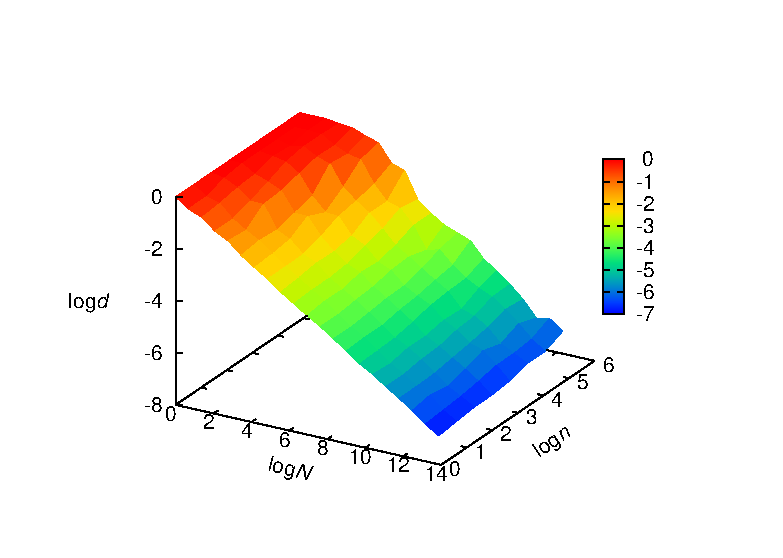
\includegraphics{figures/eps/surf/b4.eps}}}\hspace{5pt}
\subfloat[$\ell = 6$.]{
\resizebox*{6.5cm}{!}{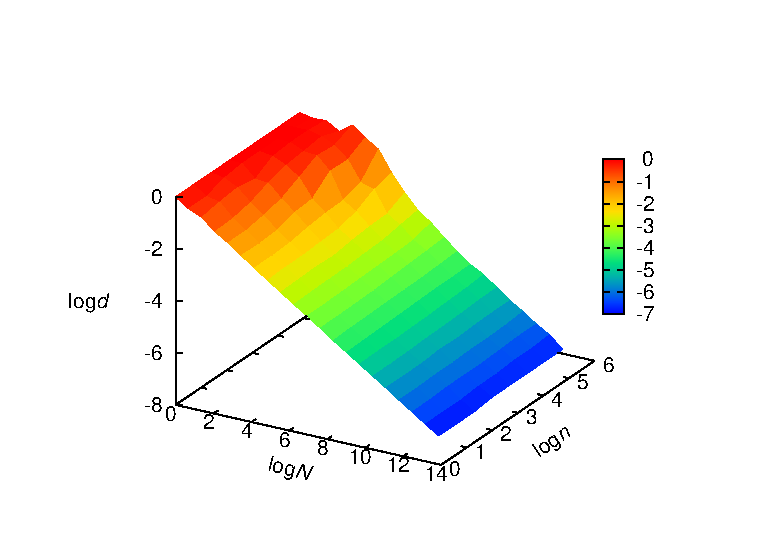
\includegraphics{figures/eps/surf/b6.eps}}}
\end{center}
  
\begin{center}
\subfloat[$\ell = 8$.]{
\resizebox*{6.5cm}{!}{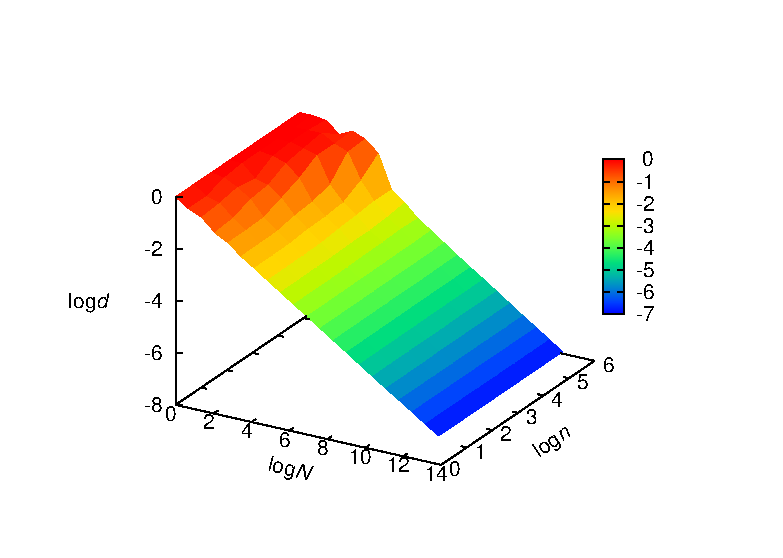
\includegraphics{figures/eps/surf/b8.eps}}}\hspace{5pt}
\subfloat[$\ell = 10$.]{
\resizebox*{6.5cm}{!}{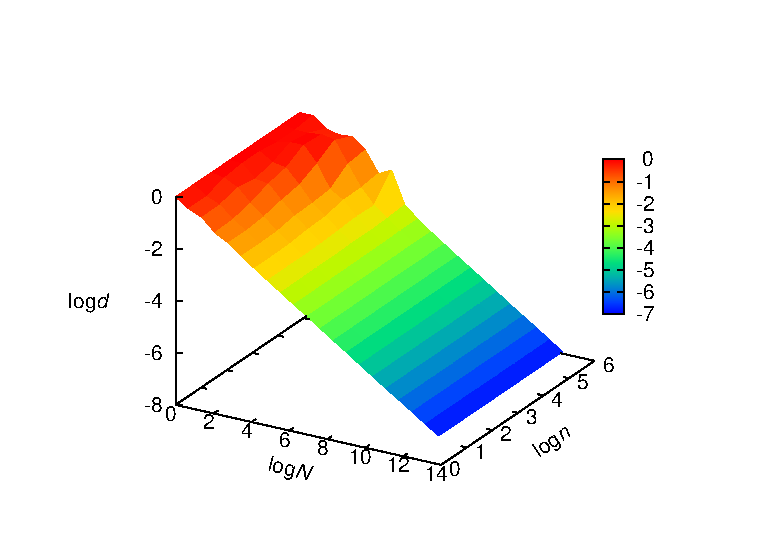
\includegraphics{figures/eps/surf/b10.eps}}}
\end{center}

\begin{center}
\subfloat[$\ell = 12$.]{
\resizebox*{6.5cm}{!}{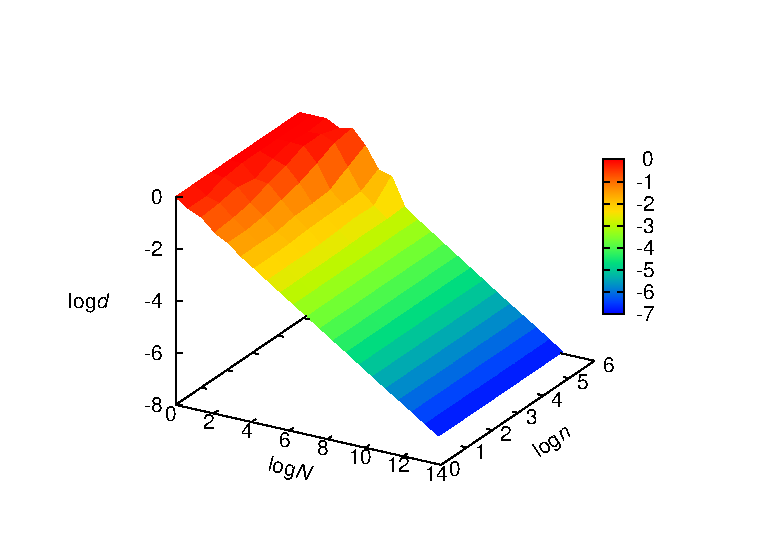
\includegraphics{figures/eps/surf/b12.eps}}}\hspace{5pt}
\subfloat[$\ell = 14$.]{
\resizebox*{6.5cm}{!}{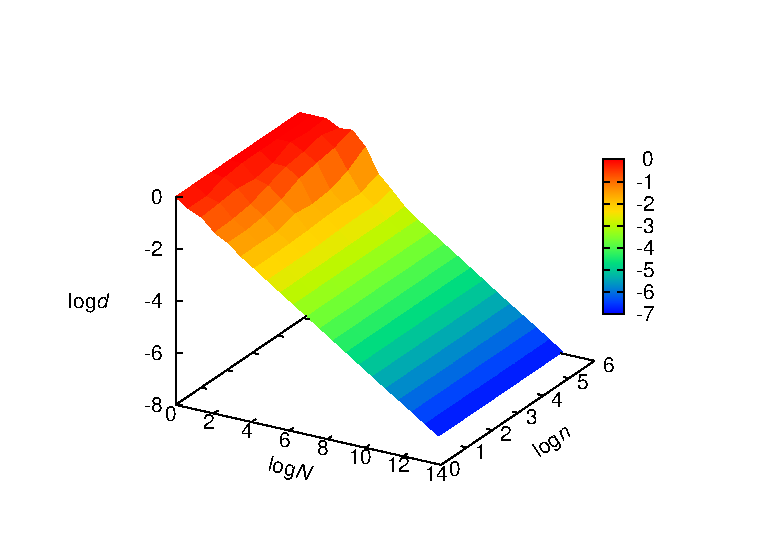
\includegraphics{figures/eps/surf/b14.eps}}}
\caption{\textbf{Convergence of finite population behaviour:} $d$ is
  distance between finite population ${\bm f}^n$ and infinite
  population ${\bm q}^n$ at generation $n$, population size $N$, for
  genome length $\ell$ (bits).}
\label{convergence}
\end{center}
\end{figure}

The data, presented in six surface graphs above and organized by
genome length, shows a near linear dependence of $\log d$ on $\log N$.
As expected, the graphs show smoothing with increasing genome length
(the computation of $d$ involves averaging over $\ell$ components),
and also with increased population size (as explained in
\cite{Vose1999}, the initial transient of a finite haploid population
trajectory converges as $N \rightarrow \infty$ to the corresponding
infinite population model).

%\newpage
  Of particular interest is the linear trend exhibited above.  The
  slope $m$ and intercept $b$ of the regression line
  \begin{equation} \label{regresion}
  \log d = m \log N + b
  \end{equation}
was computed using the data above; each was plotted against genome
length $\ell$ and organized by generation $n$. The resulting
graphs are displayed below.

\begin{figure}[H]
\begin{center}
\subfloat[Slope $m$, genome length $\ell$.]{
\resizebox*{7cm}{!}{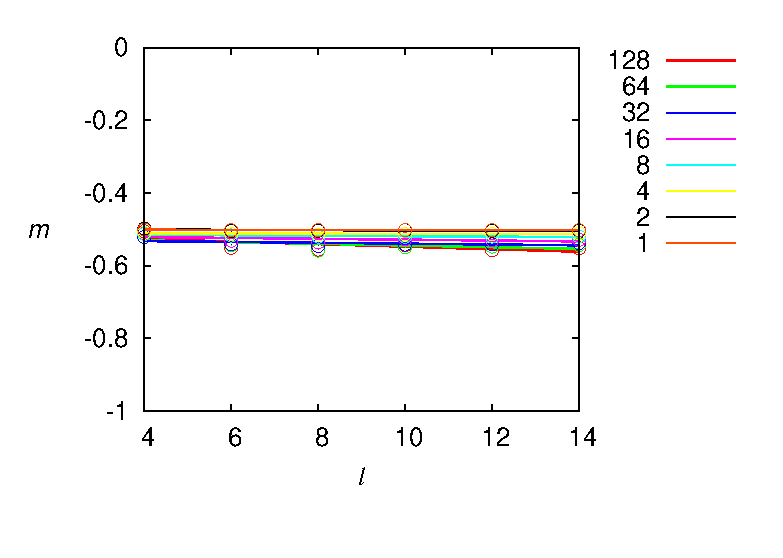
\includegraphics{figures/eps/slope/m.eps}}}\hspace{5pt}
\subfloat[Intercept $b$, genome length $\ell$.]{
\resizebox*{7cm}{!}{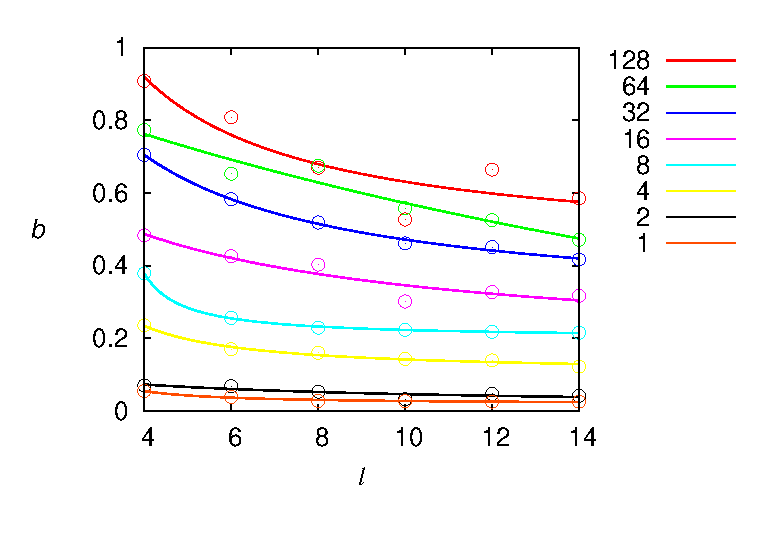
\includegraphics{figures/eps/slope/b.eps}}}
\caption{\textbf{Regression parameters:} multi-plot of slope $m$ and intercept $b$ for generation  $n \in \{1,  2,  4,  8,  16,  32,  64,  128\}$ .}
\label{regression-parameters}
\end{center}
\end{figure}

Taking the exponential of the regression line (\ref{regresion}) yields
the estimate
$d \approx N^m e^b $.

Slopes of the regression lines shown in {\bf Figure \ref{regression-parameters}} are
approximately $-0.5$, indicating
\begin{equation}
\label{covergenceDistance}
d \; \approx \; k/\sqrt{N}.
\end{equation}
 
Vose (see \cite{Vose1999}) calculated variance of next generation population with respect to expected population as 
\[
\mathcal{E}(\| \bm{q} - \mathcal{G}(\bm{p}) \|^2) = (1 - \|\mathcal{G}(\bm{p})\|^2) / \bm{N}
\] 
where $\bm{q}$ is actual population and $\mathcal{G}(\bm{p})$ is expected population.
Let $x$ be the random variable $\| \bm{q} - \mathcal{G}(\bm{p}) \|$. Let $\phi$ be the function $\phi (x) = x^2$ 
which is convex function. Then $\mathcal{E}(\| \bm{q} - \mathcal{G}(\bm{p}) \|^2)$ becomes $\mathcal{E}(\phi (x))$. 
From Jensen's Inequality (see \cite{JensenInequality}),
if $\phi$ is a convex function, then
\begin{eqnarray*}
\phi(\mathcal{E}(x))) & \leq & \mathcal{E}(\phi(x)) \\
\mathcal{E}(x) & \leq & \sqrt{\mathcal{E}(x^2)}
\end{eqnarray*}
Substituting original variables,
\begin{equation}
\label{convergenceRHS}
\mathcal{E}(\| \bm{q} - \mathcal{G}(\bm{p}) \|) \leq \sqrt{(1 - \|\mathcal{G}(\bm{p})\|^2) / \bm{N}}
\end{equation}
Equation \ref{convergenceRHS} shows the expected rate of convergence for the single-step
haploid case; the distance is inversely proportional to square root of population size. 
And equation \ref{covergenceDistance} agrees with  equation \ref{convergenceRHS}.

The consistent convergence rate
across multiple generations is somewhat surprising, simulation
results above indicate it may persist to generation $n = 128$.

The intercept graphs above show the constant of proportionality $k =
e^b$ decreases monotonically with genome length $\ell$, and increases
monotonically with generation $n$.  The increase in $k$ for larger $n$
seems to be a manifestation of the growing nonlinearity uniformly
exhibited by the plots in {\bf Figure \ref{convergence}} as $n$ increases.  It seems
likely that the nonlinearity results from genetic drift experienced by
finite populations (see \cite{CrowKimura}).









 
    \chapter{Specialization}\label{ch:specialize}
This chapter summarizes from the development in Vose \cite{Vose1999}.
It specializes the haploid evolution equations in the previous section 
to a context where mask-based crossing over and mutation operators are used, 
leading to Vose's infinite population model for Genetic Algorithms.  Whereas 
in previous sections {\em component} referred to a component
of a distribution vector $q^n$ or $p^n$, in this section a component
is either a probability (when when speaking of a component of a
distribution vector), or a bit (when speaking of a component of a
haploid).

The set of haploids (i.e., length $\ell$ binary strings) is a
commutative ring $\mathcal{R}$ under component-wise addition and
multiplication modulo $2$.  This algebraic structure is crucial to
Vose's specialization and subsequent analysis of
(\ref{model3}). Denote the additive identity by ${\bf 0}$ and the
multiplicative identity by ${\bf 1}$, and let $\overline{g}$
abbreviate ${\bf 1} + g$.  Except when explicitly indicated otherwise,
operations acting on elements of $\mathcal{R}$ are as defined in this
paragraph.\footnote{In particular, $g \overline{g} = {\bf 0} = g+g$,
  $g^2 = g$, $g + \overline{g} = {\bf 1}$ for all $g \in
  \mathcal{R}$.}

\section{Mutation}
Mutation simulates effects of error that happen with low probability during duplication of chromosome. Mutation provides mechanism to inject new strings into the next generation population which gives {\em RHS} ability to search beyond the confines of initial population.

Symbol $\mu$ is used to represent mutation distribution describing the probability $\mu_i$ with which $i \in \Omega$ is selected to be a mutation mask. $\mu : \Omega \rightarrow \Omega$ is nondeterministic mutation function where the result $\mu(x)$ of applying mutation function on $x$ is $x \oplus i$ with probability $\mu_i$ of distribution $\mu$ where $i$ is {\em mutation mask}. Mutating $x$ using mutation mask $i$ alters the bits of $x$ in those positions the mutation mask $i$ is 1.
$\mu \in [0, 0.5)$ is regarded as a {\em mutation rate} which implicitly specifies distribution $\mu$ according to rule \VoseWright1998{Vose1999}
\[
\mu_i = (\mu)^{{\bf 1}^Ti} (1-\mu)^{\ell- {\bf 1}^Ti}
\]
If $g$ should mutate to $g^\prime$ with probability $\rho$,
let\\[-0.2in]
\[
\mu_{g + g^\prime} \; = \; \rho\\[0.05in]
\]
Given distribution $\mu$, mutation is the stochastic operator sending
$g$ to $g^\prime$ with probability $\mu_{g + g^\prime}$.

Mutation considered is {\em independent} for all $j$ and $k$ which means \cite{VoseWright1998}
\[
\mu_j = \sum\limits_{k\otimes i=0} \mu_{i\oplus j} \sum\limits_{k\overline \otimes i=0} \mu_{i\otimes j}
\]

\section{Crossover}
Crossover refers to crossing over (also termed recombination) between two chromosomes (strings in our case). Crossover like mutation also provides mechanism for injection of new strings into new generation population. Masked based crossover is used in this document. Geiringer \cite{Geiringer1944} used crossover mask with probability (distribution) associated with the mask to generate offsprings from parent chromosomes in absence of mutation and selection. Let $\chi_m$ be probability distribution with which $m$ is selected to be a crossover mask.
Following Geiringer \cite{Geiringer1944}, if crossing over $u$ and $v$ should produce $u^\prime$ and $v^\prime$ with probability $\rho$, let
\[
\chi_m \; = \; \rho
\]
where $m$ is $1$ at components which $u^\prime$ inherits from $u$, and
$0$ at components inherited from $v$.  It follows that\\[-0.3in]
\begin{eqnarray*}
u^\prime & = & m \nudge u + \overline{m} \nudge\nudge v \\
v^\prime & = & m \nudge v + \overline{m} \nudge\nudge u
\end{eqnarray*}
Given distribution $\chi$, crossover is the stochastic operator which
sends $u$ and $v$ to $u^\prime$ and $v^\prime$ with probability $\chi_m/2$ for each $u^\prime$ and $v^\prime$.

$\chi$ can be considered as a {\em crossover rate} that specifies the distribution $\chi$ given by rule \cite{VoseWright1998}
\[
  \chi_i =\begin{cases}
    \chi  c_i & \text{if $i>0$}.\\
    1 - \chi + \chi  c_0 & \text{if $i = 0$}.
  \end{cases}
\]
where $c \in \Lambda$ is referred to as {\em crossover type}. Classical crossover types include {\em 1-point crossover} and {\em uniform crossover}. For {\em 1-point crossover},
\[
  c_i =\begin{cases}
    1/(\ell - 1) & \text{if $\exists k \in (0, \ell).i = 2^k - 1$}.\\
    0 & \text{otherwise}.
  \end{cases}
\]
and for uniform crossover, $c_i = 2^{-\ell}$.

\section{Mixing Matrix}
The combined action of mutation and crossover is referred to as {\em mixing}.
The {\em mixing matrix\/} $M$ is the transmission matrix corresponding to the 
additive identity of $\mathcal{R}$ is
\[
M \; = \; M_{\bf 0}\\[-0.01in]
\]
Crossover and mutation are defined in a manner respecting arbitrary partioning and arbitrary linkage to preserve the ability to endow abstract syntax with specialized semantics. Groups of loci can mutate and crossover with arbitrarily specified probabilities as disscussed in above sections. For mutation distribution $\mu$ and crossover distribution $\chi$, whether or not $\mu$ is independent if mutation is performed before crossover, then transmission function can be expressed as \cite{VoseWright1998}
\begin{equation}
\label{transmission}
t_{\langle u,v \rangle}(g) \; = \;\,
\sum_{i \nudge \in \nudge \mathcal{R}} \, \sum_{j \nudge \in \nudge \mathcal{R}} \,
\sum_{k \nudge \in \nudge \mathcal{R}}
\mu_i \nudge \mu_j \, \frac{\chi_k + \chi_{\overline{k}}}{2} \,
[\nudge k (u + i) + \overline{k}(v + j) \, = \, g\nudge]
\end{equation}
Here a child gamete $g$ is produced via mutation and then crossover (which are operators that
commute). 

The mixing matrix $M$ is a fundamental object, because (\ref{transmission}) implies that evolution equation (\ref{model3}) can be expressed in the form
\begin{equation}
\label{model4}
p_g^\prime \; = \; (\sigma_g \nudge p)^T M \, (\sigma_g \nudge p)
\end{equation}
where the permutation matrix $\sigma_g$ is defined by component equations
\[
(\sigma_g)_{u,v} \; = \; [\nudge u+v = g\nudge ]
\]

\section{Walsh Transorm}
A time series, f(t), in terms of a series of Walsh funcitons W(n,t) \cite{Beauchamp1975}, viz.
\[
f(t) = a_{0} W_{0,t} + \sum_{n=1}^{N-1} a_n W_{n,t}
\]
where $n$ is an ordering number, $N$ is number of terms used in Walsh series to express time series and
\[
\frac{a_0}{2} = \frac{1}{T} \int\limits_0^T f(t) W_{n,t} dt
\]
\[
a_n = \frac{1}{T} \int\limits_0^T f(t) W_{n,t} dt
\]

Finite discrete Walsh transform pair on N sampling points, $x_t$, can be expressed as \cite{Beauchamp1975} 
\begin{equation}
\label{WalshT}
X_n = \frac{1}{N} \sum_{t=0}^{N-1} x_t W_{n,t}
\end{equation}
\[
n = 0, 1, 2...N-1
\]
and
\[
x_t = \sum_{n=0}^{N-1} X_n W_{n,t}
\]
\[
t = 0, 1, 2...N-1
\]

The Walsh function series $W_{n,t}$ can be obtained using Walsh matrix also known as Hadamard matrix of order N. 
Walsh matrix or Hadamard matrix is a square matrix of order N whose coefficients comprise only +1 and -1 and where its rows 
(and columns) are orthogonal to one another. 
The Walsh matrix is defined by
\[
W_{n,t} = N^{-1/2} (-1)^{n \cdot t}
\]
where $N^{-1/2}$ is normalization factor and $n \cdot t$ is bitwise dot product of binary representation of number n and t.

The matrix is symmetric, i.e.,
\[
W_{n,t} = W_{n,t}
\]
and it has entries satisfying
\[
W_{n, t \oplus k} = N^{1/2} W_{n, t} W_{n, k}
\]

The practical importance of this symmetry is that the transform and inverse represent same mathematical operation, hence simplifying the derivation and application of the transform. With the normalized form, \textit{Walsh matrix} is its own inverse, i.e.,
\[
W = W^{-1}
\]

In the matrix form, given vector $w$ and matrix $A$, let $\widehat{w}$ and
$\widehat{A}$ denote the Walsh transform of $w$ and $A$ respectively. Then $\widehat{w} = Ww$ and
$\widehat{A} = WAW$. If $w$ is a row vector, then $w$ in its Walsh basis $\widehat{w}$ represents $wW$.

\section{Walsh Transform Adaptation}
The Walsh transform has spectacular ability to unravel the intricacies of mixing. And that is why we adapt Walsh transform methods for computing evolutionary trajectories, which have already been established for Vose's haploid model \cite{VoseWright1998}. Adaptation of Walsh transformation efficiently models infinite diploid population evolution. This adaptation of Walsh transormation helps in making feasible comparisons between finite and infinte diploid population short-term evolutionary behavior.
Recalling evolution equation (\ref{model4}), without selection, specialized to Vose's infinite population model expressed in mixing matrix's term,
\[
p_g^\prime \; = \; (\sigma_g \nudge p)^T M \, (\sigma_g \nudge p)
\]
where the permutation matrix $\sigma_g$ is defined by component
equations
\[
(\sigma_g)_{u,v} \; = \; [\nudge u+v = g\nudge ]
\]

In our model, the Walsh matrix $W$
is defined by component equations
\[
W_{u,v} \; = \; 2^{-\ell/2} (-1)^{u^T v}
\]
where the subscripts \nudge u, \nudge v (which belong to $\mathcal{R}$) on the left hand side are interpreted on the right hand side as column vectors in $\mathbb{R}^{\ell}$.
Columns of $W$ form the orthonormal basis --- the
{\em Walsh basis\/} --- which simultaneously diagonalizes the
$\sigma_g$.

A change of basis which simultaneously diagonalizes the $\sigma_g$
unravels the evolution equation (\ref{model4}).  
Expressed in the Walsh basis (see \cite{Vose1999}), the mixing matrix
takes the form
\begin{equation}
\label{Mhat}
\widehat{M}_{u,v} \; = \; 2^{\,\ell-1} \,[\nudge u \nudge v = {\bf
    0}\nudge]\, \widehat{\mu}_u \nudge \widehat{\mu}_v \!  \sum_{k
  \nudge \in \nudge \overline{u+v} \nudge \mathcal{R}} \chi_{k + u} +
\chi_{k + v}
\end{equation}
and equation (\ref{model4}) takes the form
\begin{equation}
\label{model5}
\widehat{p}_g^{\,\,\prime} \; = \; 2^{\,\ell/2} \sum_{i \nudge \in \nudge g \mathcal{R}}
\widehat{p}_i \, \nudge \widehat{p}_{i+g} \,\widehat{M}_{i,i+g}
\end{equation}
where $g \mathcal{R} = \{g \nudge i \, | \, i \in \mathcal{R} \}$ (for
any $g \in \mathcal{R}$).

The mapping from generation $n$ to generation $n+1$, determined in
natural coordinates by equation (\ref{model3}) in terms of the
transmission function (\ref{Mg}), and given in Walsh coordinates by
equation (\ref{model5}) in terms of the mixing matrix (\ref{Mhat}), is
Markovian; the next state $p^\prime$ depends only upon the current
state $p$.  Let $\mathcal{M}$ represent the mixing transformation,
\begin{equation} \label{mixing_transformation}
p^\prime \; = \; \mathcal{M}(p)
\end{equation}
and let $\mathcal{M}^n(p)$ denote the $n$-fold composition of
$\mathcal{M}$ with itself; thus generation $n+1$ is described by
\[
p^{n+1} \; = \; \mathcal{M}^n(p^1)
\]
where $p^1 = \pi (q^1)$.  We have little to say
about the matrix of the Markov chain corresponding to the mixing
transformation $\mathcal{M}$, because it is uncountable; each state is
a distribution vector $p$ describing a population. However, that is
not an obstacle to computing evolutionary trajectories;
(\ref{mixing_transformation}) can be computed in Walsh coordinates
relatively efficiently via (\ref{Mhat}) and (\ref{model5}).

\section{Fast Walsh Transform}
However, computation of discrete Walsh transform given by equation (\ref{WalshT}) takes $N^2$ operations (addition or subtraction).
An algorithm using matrix factorization techniques is found to perform transformation in $N \log_2 N$ operations.
This algorithm in fast Walsh transform (FWT). 
Shanks \cite{Shanks1969} described FWT algorithm which is analogous to Cooley-Tukey \cite{CooleyTukey1965} algorithm for fast Fourier transformation. Shanks assumed walsh function to be periodic with period $N$, where $N$ is an integral power of 2. So a complete orthogonal set will have $N$ function $W_{m,n}$ where $m = 0, 1, 2,.., N-1$ and $n = 0, 1, 2,.., N-1$. The first two discrete walsh functions are defined as 
\begin{equation}
\label{FWT1}
W_{0,n} = 1    \text{ for $n = 0, 1, 2,.., N-1$}
\end{equation}
\begin{equation}
\label{FWT2}
W_{1,n} = \begin{cases}
    1 & \text{for $n = 0, 1, 2,.., (N/2)-1$}.\\
    -1 & \text{for $n = N/2, (N/2)+1,.., N-1$}.
  \end{cases}
\end{equation}

Remainder of set can be generated by using multiplicative iterative equation (\ref{FWTIterative}): 
\begin{equation}
\label{FWT3}
W_{m,n} = W_{[m/2],2n}\cdot W_{m-2[m/2], n}
\end{equation}
where $[m/2]$ indicates the integer part of $m/2$.

The discrete Walsh functions as defined here are symmetric with respect to the argument (m, n). That is,
\[
W_{m, n} = W_{n,m}.
\]

For real array of length $N$, Walsh transform can be defined as 
\begin{equation}
\label{FWT4}
F(m) = \sum\limits_{n=0}^{N-1} f(n) W_{m,n}, \text{where $m = 0, 1, 2,.., N-1$}
\end{equation}

Similarly, for inverse transform is
\begin{equation}
\label{FWT5}
f(n) = \frac{1}{N}\sum\limits_{m=0}^{N-1} F(m) W_{m,n}, \text{where $n = 0, 1, 2,.., N-1$}
\end{equation}

Since walsh functions $W_{m,n}$ have values either $1$ or $-1$, computation of (\ref{FWT4}) and (\ref{FWT5}) does not require multiplication.
Shanks \cite{Shanks1969} derived using (\ref{FWT3}) an algorithm analogous to Cooley-Tukey algorithm that will require $N \log_2 N$ summations to compute complete Walsh transform. \linebreak
For $N = 8$ (which can be extended to general case),\linebreak
indices in (\ref{FWT4}) can be replaced with a set which can only have values 0 and 1. That is, 
\begin{equation}
\label{FWT6}
m = 4j_2 + 2j_1 + j_0, \text{$j_2, j_1, j_0 = 0$ or $1$}
\end{equation}
\begin{equation}
\label{FWT7}
n = 4k_2 + 2k_1 + k_0, \text{$k_2, k_1, k_0 = 0$ or $1$}
\end{equation}
Using these new notations, $W_{m,n}$ becomes $W(j_2,j_1,j_0;k_2,k_1,k_0)$. So (\ref{FWT4}) becomes 
\begin{equation}
\label{FWT8}
F(j_2,j_1,j_0) = \sum\limits_{k0 = 0}^1 \sum\limits_{k1 = 0}^1 \sum\limits_{k2 = 0}^1 f(k2,k1,k0) \cdot W(j_2,j_1,j_0;k_2,k_1,k_0)
\end{equation}

Here, $j_2,j_1,j_0$ is binary representation of $m$. So, dividing $m$ by $2$ equivalents to shifting binary representation of $m$ by $1$ to the right and dropping fractional bit. That is, if 
\[
m \leftrightarrow j_2j_1j_0
\]
then,
\[
[m/2] \leftrightarrow 0j_2j_1.
\]

Similarly, if
\[
n \leftrightarrow k_2k_1k_0
\]
then,
\[
2n \leftrightarrow k_2k_1k_00.
\]
An 8-length Walsh function is periodic with period 8. Thus any index (such as $2n$) can be evaluated modulo 8. This is equivalent to deleting any bits above the third bit and we have 
\[
2n(modulo 8) \leftrightarrow k_1K_00
\]

Using these indices, (\ref{FWT3} becomes
\begin{equation}
\label{FWT9}
W(j_2,j_1,j_0;k_2,k_1,k_0) = W(0,j_2,j_1;k_1,k_0,0) \cdot W(0,0,j_0;k_2,k_1,k_0).
\end{equation}

$j_0$ can only be 0 or 1, so $W(0,0,j_0; k_2, k_1, k_0)$ represents either $W_{0,n} or W_{1,n}$. The function $W_{0,n}$ is 1 for all $n$. And function $W_{1,n}$ is 1 if $0<n<4$ and $W_{1,n}$ is -1.0 if $4<n<7$. Thus, from (\ref{FWT7}), $W_{1,n}$ is +1.0 if $k_2=0$ and $W_{1,n}$ is -1.0 if $k_2 = 1$. Therefore, 
\begin{equation}
\label{FWT10}
W(0,0,j_0;k_2,k_1,k_0) = (-1)^{j_0k_2}.
\end{equation}

(\ref{FWT9}) can be used to factor $W(0,j_2,j_1;k_1,k_0,0)$ to get
\begin{equation}
\label{FWT11}
W(0,j_2,j_1;k_1,k_0,0) = W(0,0,j_2;k_0,0,0) \cdot W(0,0,j_1;k_1,k_0,0).
\end{equation}

Using (\ref{FWT10}) and (\ref{FWT11}) in (\ref{FWT9}), we get completely factored expression for the 8-length Walsh function
\begin{equation}
\label{FWT12}
W(j_2,j_1,j_0;k_2,k_1,k_0) = (-1)^{j_2k_0}(-1)_{j_1k_1}(-1)^{j_0k_2}.
\end{equation}

Using (\ref{FWT12}), (\ref{FWT8}) becomes 
\begin{equation}
\label{FWT13}
F(j_2,j_1,j_0;k_2,k_1,k_0) = \sum\limits_{k_0=0}^1 (-1)^{j_2k_0} \sum\limits_{k_1=0}^1 (-1)^{j_1k_1}  \cdot  \sum\limits_{k_2=0}^1 (-1)^{j_0k_2} f(k_2,k_1,k_0).
\end{equation}

We can define
\begin{equation}
\label{FWT14}
A_1(j_0,k_1,k_0) = \sum\limits_{k_2=0}^1 (-1)^{j_0k_2} f(k_2,k_1,k_0)
\end{equation}

Array $A_1$ is first set of intermediate calculations to compute $F(m)$. $A_2(j_0,j_1,k_0)$ can be computed from $A_1$ and final result $A_3(j_0,j_1,j_2)$ from $A_2$ for 8-length Walsh transform. However, the order of the values will be in the bit reversed form. It can be generalized for the case $N = 2^p$ by defining intermediate Walsh transform arrays as
\begin{equation}
\label{FWT15}
A_l(j_O,j_1,...,j_{l-1},k_{p-l-1},...,k_0) = \sum\limits_{k_{p-l}=0}^1 A_{l-1}(j_0,j_1,...,j_{l-2},k_{p-l},k_{p-l-1},...,k_0) \cdot (-1)^{j_{l-1}k_{p-l}}
\end{equation}
where $l = 1,2,...,p$ and 
\begin{equation}
\label{FWT16}
A_0(k_{p-1},k_{p-2},...,k_0) = f(k_{p-1},k_{p-2},...,k_0).
\end{equation}

The general equation for the $M= 2^P$-length discrete Walsh function is 
\[
W(j_{p-1},j_{p-2},...,j_0;k_{p-1},k_{p-2},...,k_0) = \prod_{i=0}^{p-1} (-1)^{j_{p-1-i}k_i}.
\]




    \chapter{Violation} \label{ch:evolutionary limits}
The results from chapter \ref{ch:oscillation} show that oscillation occurs
when the crossover distribution $\bm{\chi}$, and the mutation distribution $\bm{\mu}$ 
satisfy condition \ref{OscCond}. This chapter explores the robustness of finite population oscillation. 
If the finite population GA is an ergodic Markov chain, then perfect oscillation should not occur. Does approximate oscillation 
in finite populations occur in practice if condition \ref{OscCond} is violated? 
This chapter explores the  
third research question, whether finite populations exhibit approximate oscillation when the Markov chain 
is ergodic.

Error $\bm{\epsilon}$ is introduced to $\bm{\mu}$ and $\bm{\chi}$ distributions so as to 
violate condition \ref{OscCond}. Consequently, $\bm{p}^\ast \;=\; \bm{q}^\ast \;=\; \bm{z}^\ast$. 
Violation of condition \ref{OscCond} in the distributions makes the Markov chain ergodic. The initial population is 
computed using same procedure as described in section \ref{InitPopOsc}. To explore the effects of the degree  
of violation of condition \ref{OscCond} in $\bm{\mu}$ and $\bm{\chi}$, different values of $\bm{\epsilon}$ are used in experiments. 
String length $\ell \;\in\; \{8, 10, 12, 14\}$ are considered for simulation.
Going forward, we use `limit $\bm{z}^\ast$' to denote evolutionary limit when mutation distribution $\bm{\mu}$ or crossover distribution 
$\bm{\chi}$ violates condition \ref{OscCond}, and 
`non-violation limits $\bm{p}^\ast$ and $\bm{q}^\ast$' to denote limits without violation.

\section{Violation in Mutation Distribution}
The mutation distribution $\bm{\mu}$ is modified as follows
\[
\bm{\mu}_i = (1-\bm{\epsilon}) \bm{\mu}_i \nudge; \tabspace i = \{0, 1, 2,.., 2^{\ell}-1\}.
\]
Thus summing components of $\bm{\mu}$ distribution yields, 
\[
1-\bm{\epsilon} = \sum \limits_{i=0}^{2^{\ell}-1} \bm{\mu}_i
\]
Then set
\[
\bm{\mu}_0 = \bm{\epsilon}
\]
% \[
% \bm{\mu}_0 = (1-\bm{\epsilon})\bm{\epsilon}
% \]
% $c$ is total number components in $\bm{\mu}$ satisfying condition $\bm{\mu}_i = 0$ and set those components value as
% \[
% \bm{\mu}_i = \bm{\epsilon}^2/c \; ; \; where \; \bm{\mu}_i = 0
% \]
The modified mutation distribution $\bm{\mu}$ is normalized such that  $\sum \bm{\mu}_i \;=\; 1$.
The modification described above makes it possible for any population member to mutate to any other population member.
% provided there is non crossover. From equation \ref{ChiDist}, $k \bar{g} \;=\; k$ is true for any $g$ when $k$ is all $0$s, 
% and so we have positive non crossover probability present in all conditions. 
Let us exlore for two cases of $g$ in \ref{OscCond}:

1. When $g$ is all $1$s:\newline
Any mask with a $1$ at position $k$ ($0 \leq k < \ell$) and $0$ at all other positions can mutate the $k$th bit, and since the 
all $0$s mask has positive probability, strings have an option to not mutate. This makes possibile for any string to mutate to 
any other string. Let us take an example with $\ell \;=\; 8$. Let $g \;=\; 11111111$. Then, mask 
$i \;=\; 00000100$ will have positive probability according to condition \ref{OscCond}. 
Mask $i$ can be used to mutate the sixth bit of a population member. More generally, 
any bit has the option of mutating or not, so any string can mutate to any other.

2. When $g$ has atleast one $0$:\newline
Any mask with a $1$ at position $k$ and $0$ at all other positions  
will have positive probability if $g$ also is $1$ at position $k$. Thus any bit where $g$ is $1$ has the option of mutating or not.  
Any mask with $1$ in just one of the positions where $g$ has $1$s and also $1$ in just one of the positions where $g$ has $0$s can be used to 
mutate a bit where $g$ is $0$. Let us take an example with $\ell \;=\; 8$. Let $g \;=\; 11001111$. Then, 
mask $i \;=\; 00000100$ will have positive probability according to condition \ref{OscCond}. Also mask 
$j \;=\; 00010100$ will have positive probability. Mask $i$ can be used to mutate the sixth bit, and masks $i$ and $j$ will result in mutating
the fourth bit. More generally, any bit has the option of mutating or not, so any string can mutate to any other. Since any population can therefore 
mutate to any other population (this may involve many generations because there are many population members which may need to be mutated), the Markov 
chain is irreducible.

The Markov chain is also aperiodic. We prove this by simple induction. 
Let $S(n)$ be the assertion that population $P$ can be returned to in $n$ generations. 
Our base case is $n \;=\; 1$. The GA can stay in its original state $P$ if no mutation or crossover events occur. 
Population $P$ has option to not mutate to any other population, since all $0$s mutation mask 
has positive probability. Moreover, the all $0$s crossover mask can have positive probability since 
that is compatible with condition \ref{OscCond}.
So $S(n)$ is true. Now, assume $S(k)$ is true. Therefore, population $P$ can be returned to in $n \;= \;k$ generations. 
In the $k+1$th generation, population $P$ has the option to stay in state $P$. 
So $S(K+1)$ is also true and that completes the inductive proof. 
Since any population state can be returned to in any period of time, the Markov chain is aperiodic. 

Because the Markov chain formed by GA is irreducible and aperiodic, 
the Markov chain is ergodic (see \cite{MarkovChain}), and a steady state distribution 
with positive components exists for the GA.   

Simulations were repeated with the violations in (\ref{OscCond}) described above for the mutation distribution.
The distances of both infinite and finite populations to limit $\bm{z}^\ast$ were plotted. 
The distances of both infinite and finite populations to non-violation limits $\bm{p}^\ast$ and $\bm{q}^\ast$ were also plotted.

% figures for mu violation
\subsection{Haploid Population $\mathtt{\sim}$ $\epsilon: 0.01$}
% l = 8
\begin{figure}[h]
\begin{center}
\subfloat{
\resizebox{8cm}{5cm}{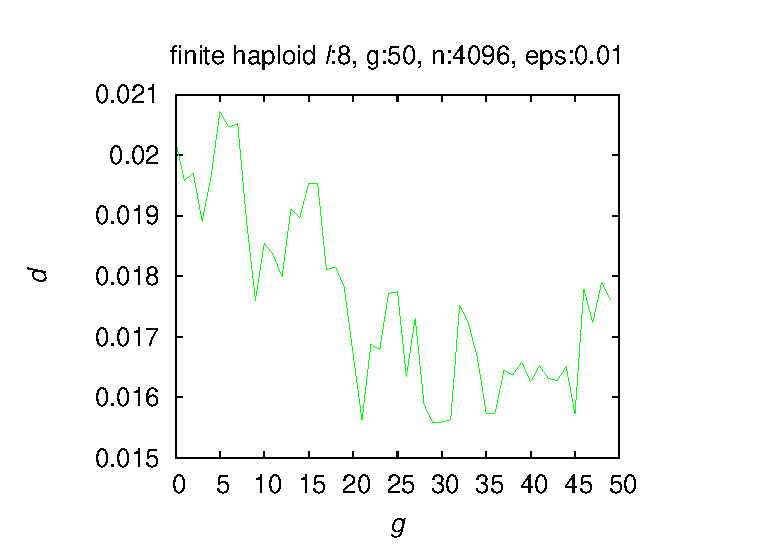
\includegraphics{figures/eps/vio/mu/b8/e0.01/n00004096_fin_hap.eps}}} \hspace{-3em}%
\subfloat{
\resizebox{8cm}{5cm}{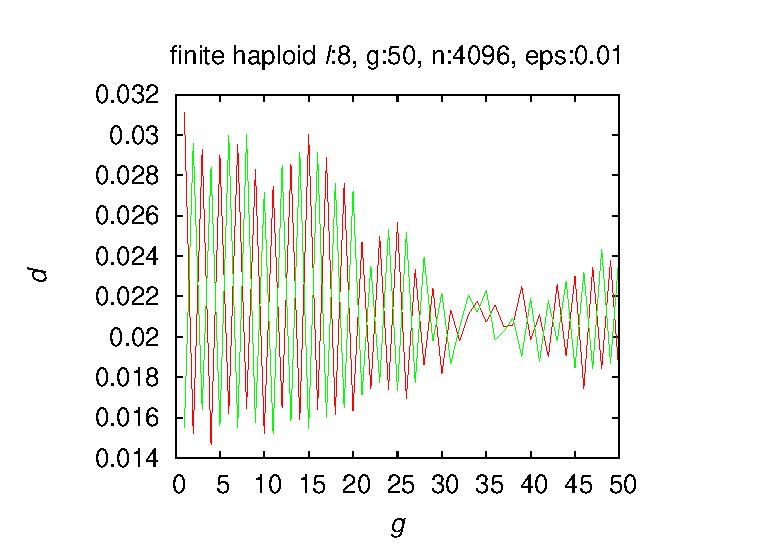
\includegraphics{figures/eps/vio/mu/b8/e0.01/n00004096_fin_hap_wovio.eps}}}\vspace{-1em} \hspace{-3em}%
\end{center}
\begin{center}
\subfloat{
\resizebox{8cm}{5cm}{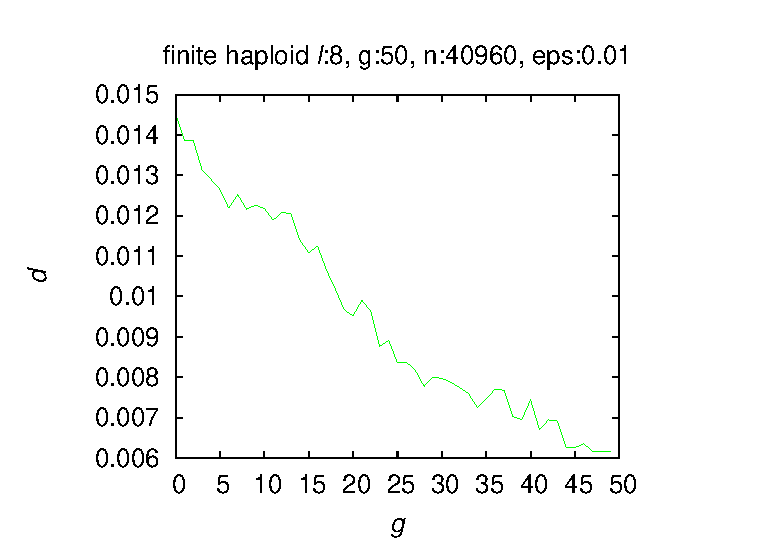
\includegraphics{figures/eps/vio/mu/b8/e0.01/n00040960_fin_hap.eps}}} \hspace{-3em}%
\subfloat{
\resizebox{8cm}{5cm}{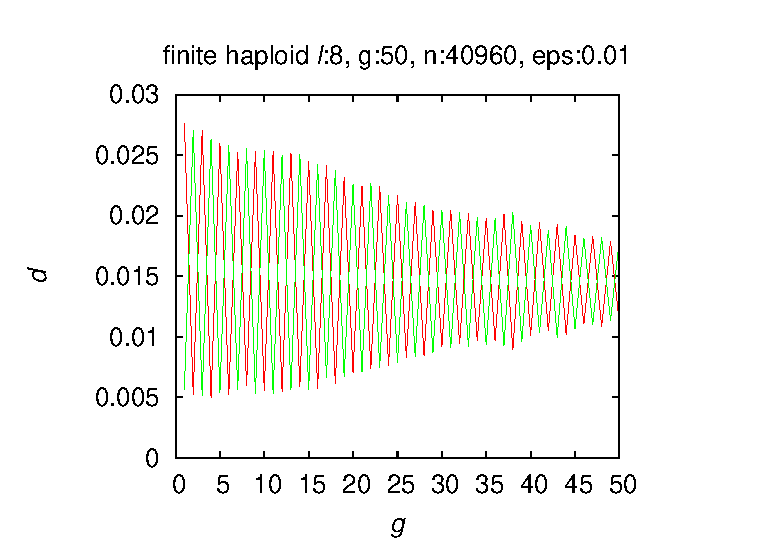
\includegraphics{figures/eps/vio/mu/b8/e0.01/n00040960_fin_hap_wovio.eps}}}\vspace{-1em} \hspace{-3em}%
\end{center}

\begin{center}
\subfloat{
\resizebox{8cm}{5cm}{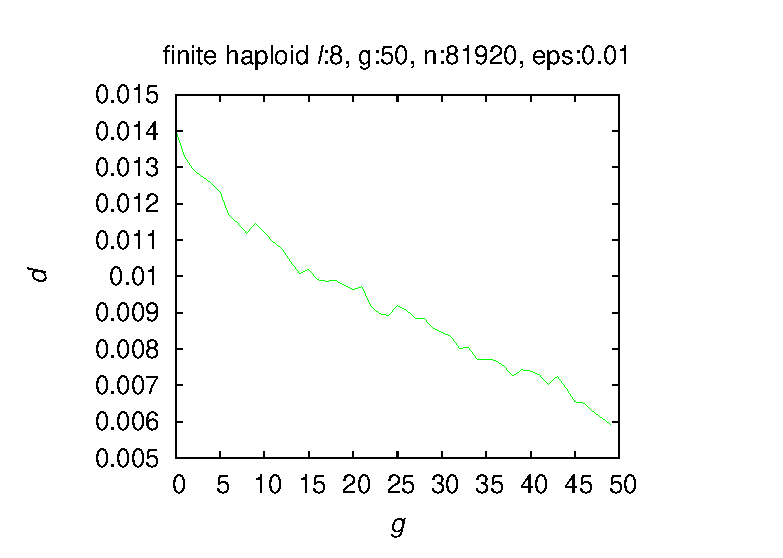
\includegraphics{figures/eps/vio/mu/b8/e0.01/n00081920_fin_hap.eps}}} \hspace{-3em}%
\subfloat{
\resizebox{8cm}{5cm}{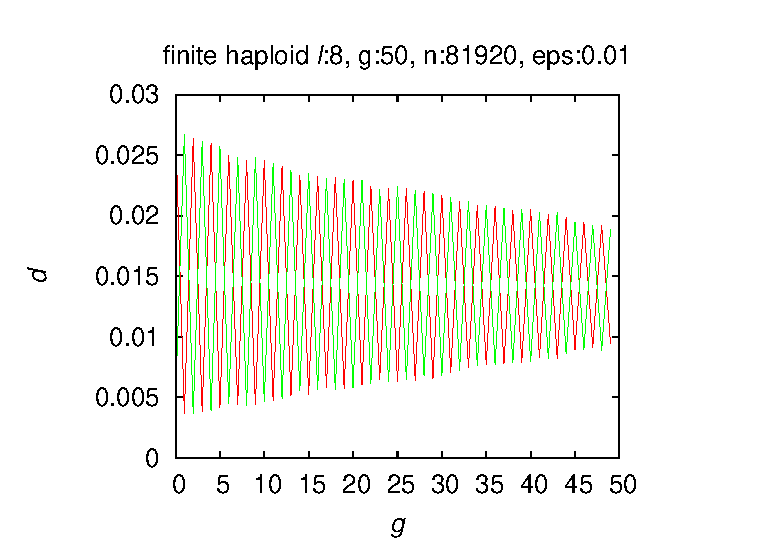
\includegraphics{figures/eps/vio/mu/b8/e0.01/n00081920_fin_hap_wovio.eps}}}\vspace{-1em} \hspace{-3em}%
\end{center}

\begin{center}
\subfloat{
\resizebox{8cm}{5cm}{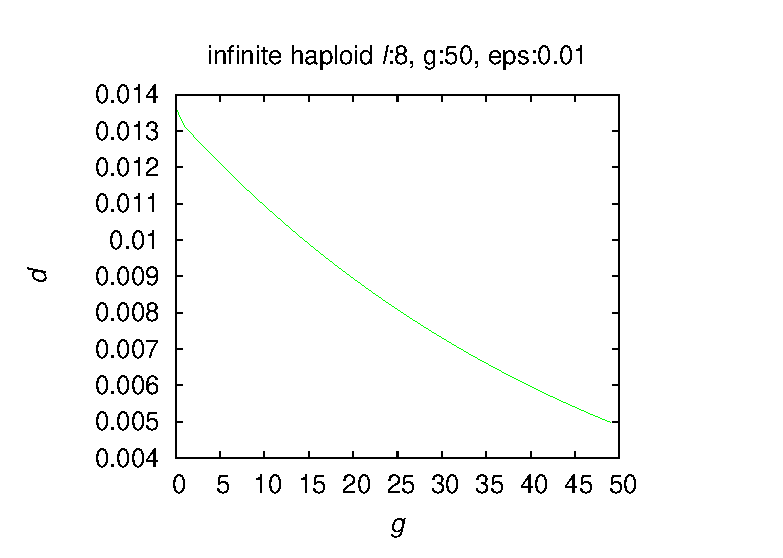
\includegraphics{figures/eps/vio/mu/b8/e0.01/inf_hap.eps}}}\hspace{-3em}%
\subfloat{
\resizebox{8cm}{5cm}{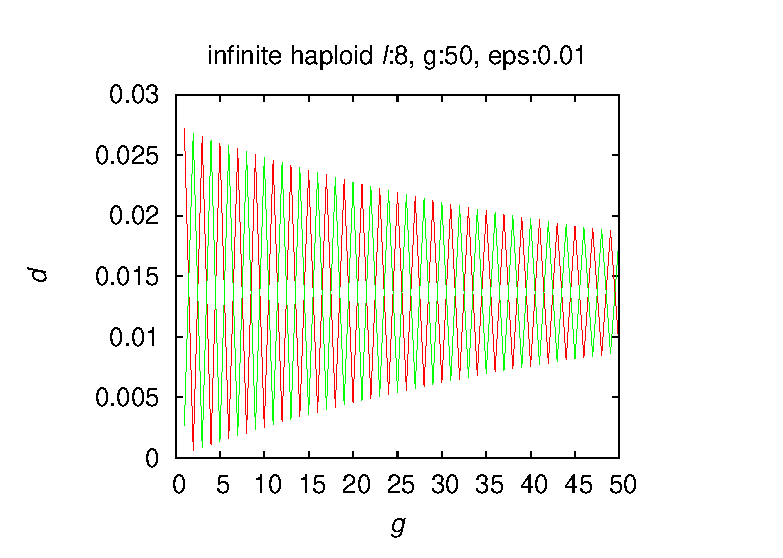
\includegraphics{figures/eps/vio/mu/b8/e0.01/inf_hap_wovio.eps}}}\vspace{-0.5em} \hspace{-3em}%
\caption{\textbf{Infinite and finite haploid population oscillation behavior in case of violation in $\bm{\mu}$ for genome length $\ell = 8$ and $\bm{\epsilon} = 0.01$:} 
  In left column, $d'$ is distance of finite population of size $n$ or infinite population to limit $\bm{z}^\ast$ for $g$ generations. In right column, $d$ is distance of finite population or infinite population to limits $\bm{p}^\ast$ and $\bm{q}^\ast$ without violation.}
\label{oscillation_8h_vio_mu_0.01}
\end{center}
\end{figure}

% l = 10

\begin{figure}[h]
\begin{center}
\subfloat{
\resizebox{8cm}{5cm}{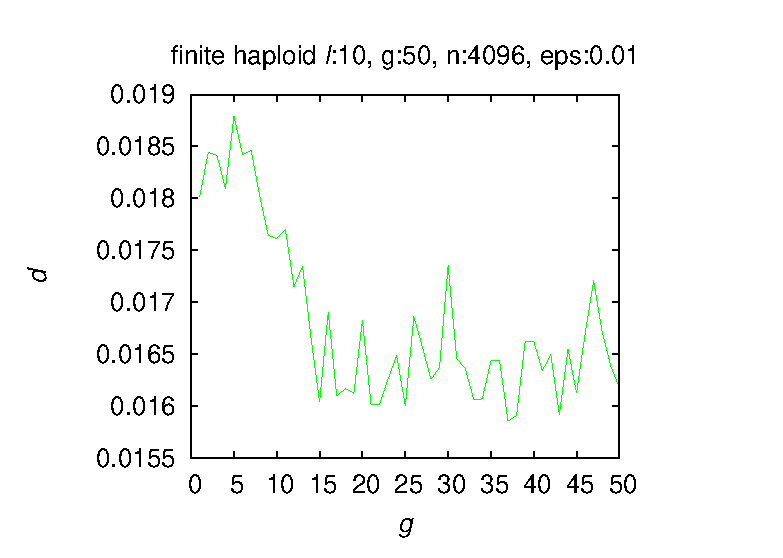
\includegraphics{figures/eps/vio/mu/b10/e0.01/n00004096_fin_hap.eps}}} \hspace{-3em}%
\subfloat{
\resizebox{8cm}{5cm}{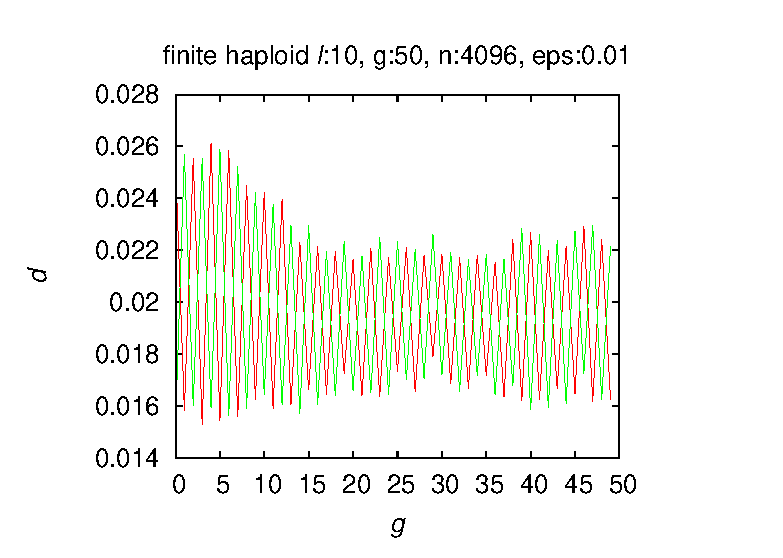
\includegraphics{figures/eps/vio/mu/b10/e0.01/n00004096_fin_hap_wovio.eps}}}\vspace{-1em} \hspace{-3em}%
\end{center}
\begin{center}
\subfloat{
\resizebox{8cm}{5cm}{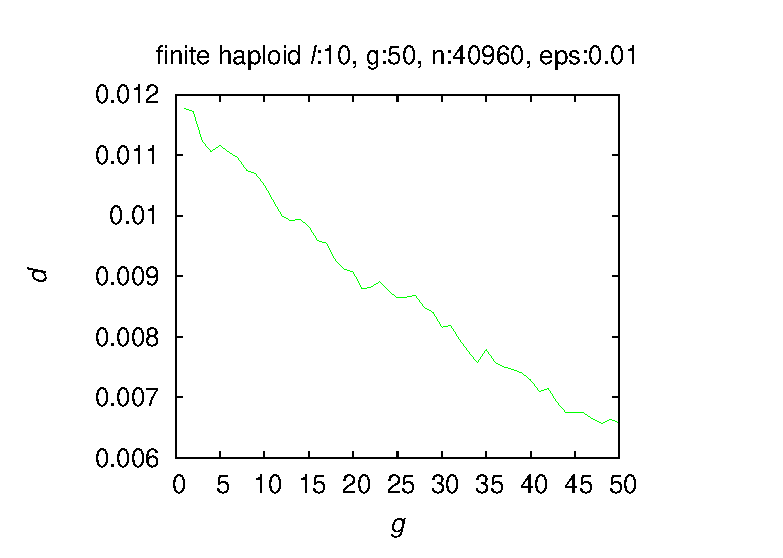
\includegraphics{figures/eps/vio/mu/b10/e0.01/n00040960_fin_hap.eps}}} \hspace{-3em}%
\subfloat{
\resizebox{8cm}{5cm}{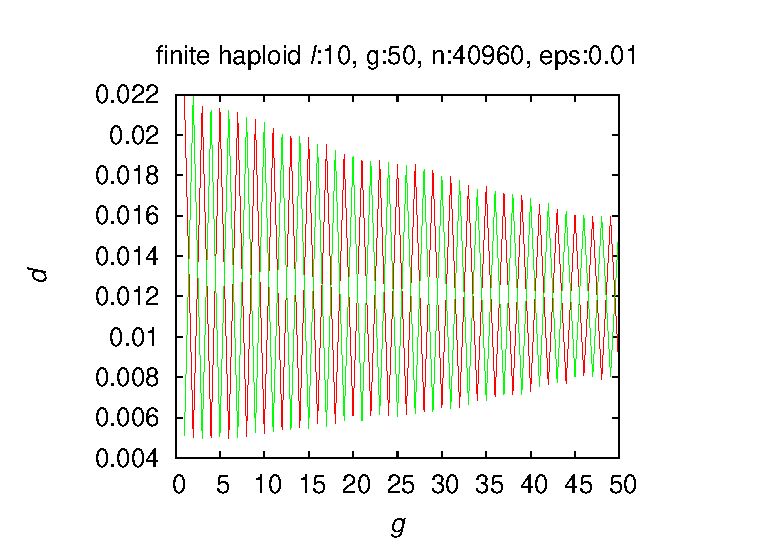
\includegraphics{figures/eps/vio/mu/b10/e0.01/n00040960_fin_hap_wovio.eps}}}\vspace{-1em} \hspace{-3em}%
\end{center}

\begin{center}
\subfloat{
\resizebox{8cm}{5cm}{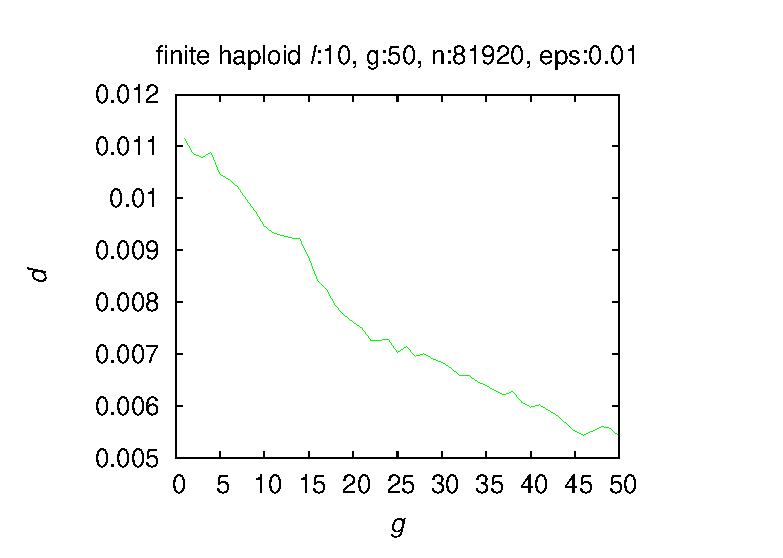
\includegraphics{figures/eps/vio/mu/b10/e0.01/n00081920_fin_hap.eps}}} \hspace{-3em}%
\subfloat{
\resizebox{8cm}{5cm}{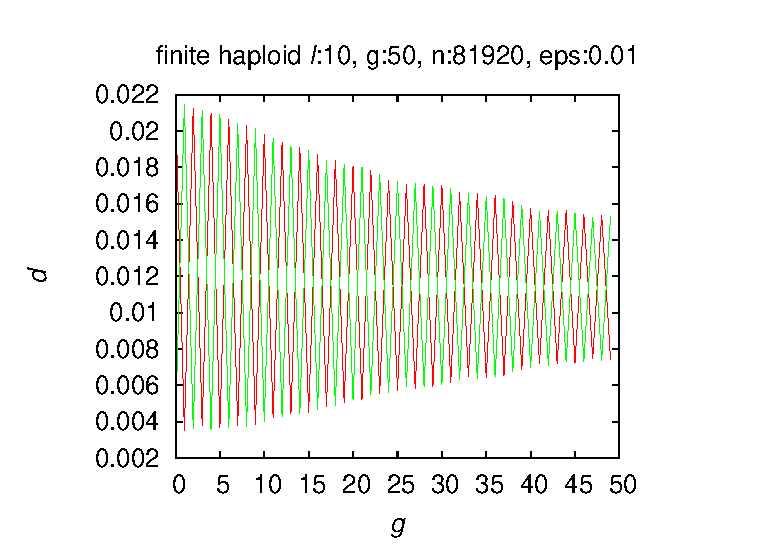
\includegraphics{figures/eps/vio/mu/b10/e0.01/n00081920_fin_hap_wovio.eps}}}\vspace{-1em} \hspace{-3em}%
\end{center}

\begin{center}
\subfloat{
\resizebox{8cm}{5cm}{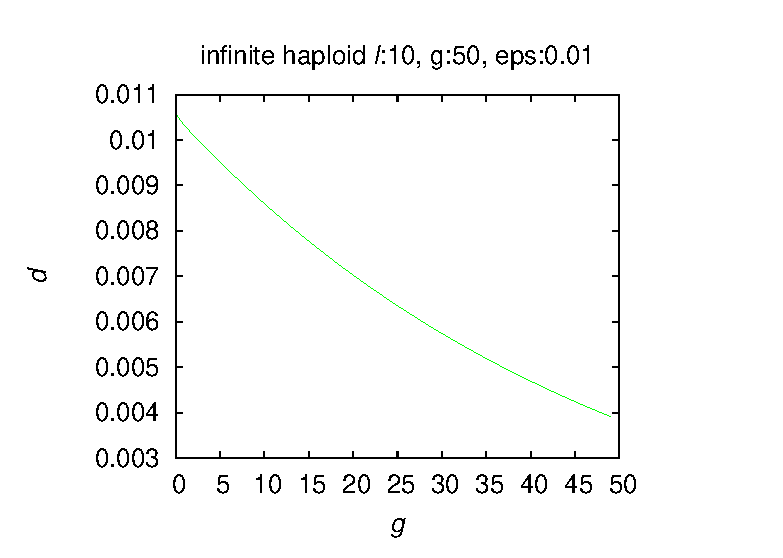
\includegraphics{figures/eps/vio/mu/b10/e0.01/inf_hap.eps}}}\hspace{-3em}%
\subfloat{
\resizebox{8cm}{5cm}{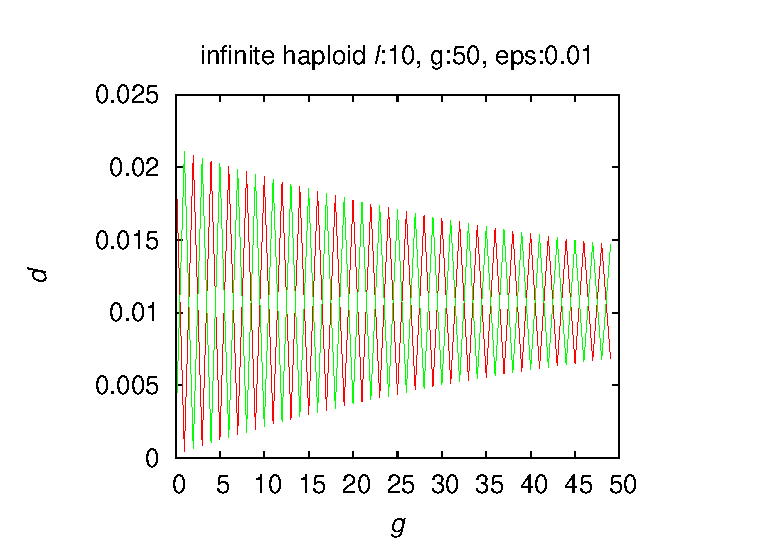
\includegraphics{figures/eps/vio/mu/b10/e0.01/inf_hap_wovio.eps}}}\vspace{-0.5em} \hspace{-3em}%
\caption{\textbf{Infinite and finite haploid population oscillation behavior in case of violation in $\bm{\mu}$ for genome length $\ell = 10$ and $\bm{\epsilon} = 0.01$:} 
  In left column, $d'$ is distance of finite population of size $n$ or infinite population to limit $\bm{z}^\ast$ for $g$ generations. In right column, $d$ is distance of finite population or infinite population to limits $\bm{p}^\ast$ and $\bm{q}^\ast$ without violation.}
\label{oscillation_10h_vio_mu_0.01}
\end{center}
\end{figure}

% l = 12

\begin{figure}[h]
\begin{center}
\subfloat{
\resizebox{8cm}{5cm}{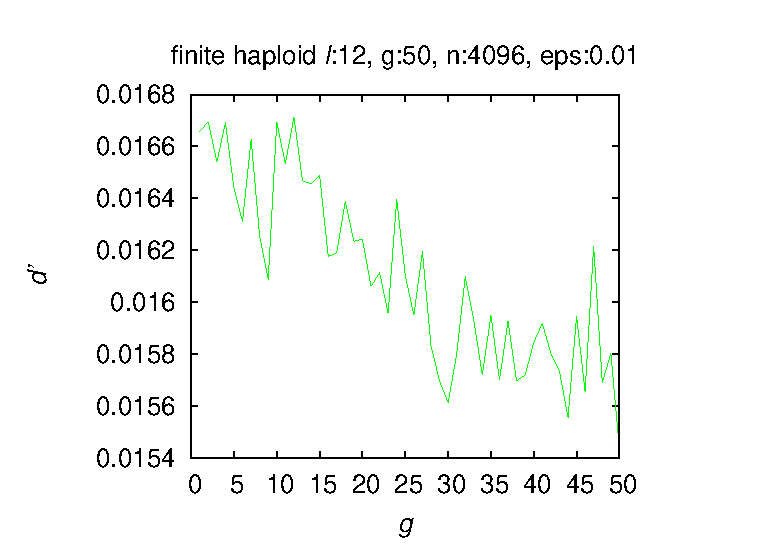
\includegraphics{figures/eps/vio/mu/b12/e0.01/n00004096_fin_hap.eps}}} \hspace{-3em}%
\subfloat{
\resizebox{8cm}{5cm}{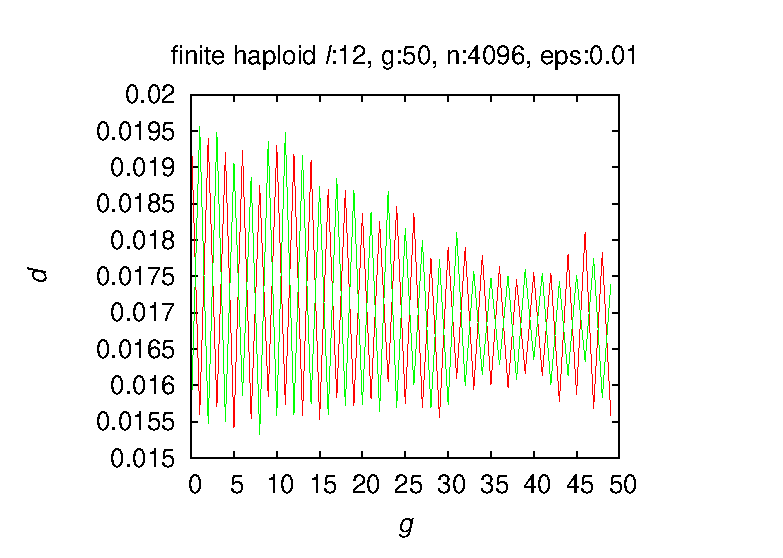
\includegraphics{figures/eps/vio/mu/b12/e0.01/n00004096_fin_hap_wovio.eps}}}\vspace{-1em} \hspace{-3em}%
\end{center}
\begin{center}
\subfloat{
\resizebox{8cm}{5cm}{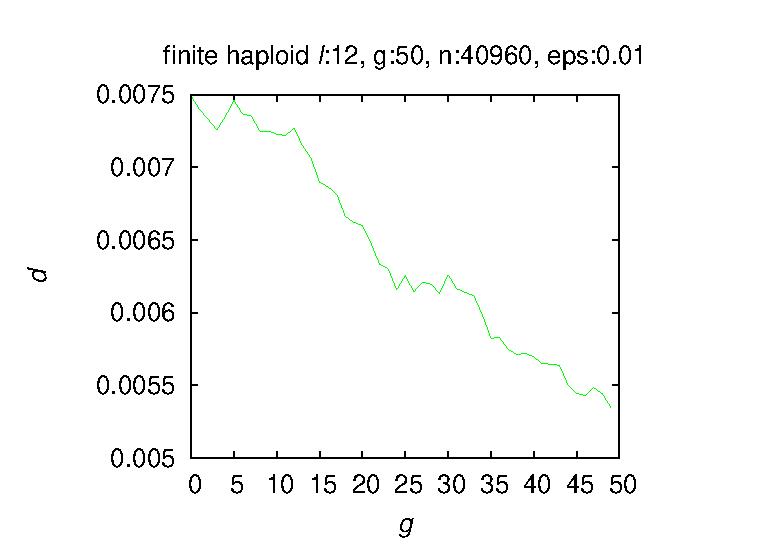
\includegraphics{figures/eps/vio/mu/b12/e0.01/n00040960_fin_hap.eps}}} \hspace{-3em}%
\subfloat{
\resizebox{8cm}{5cm}{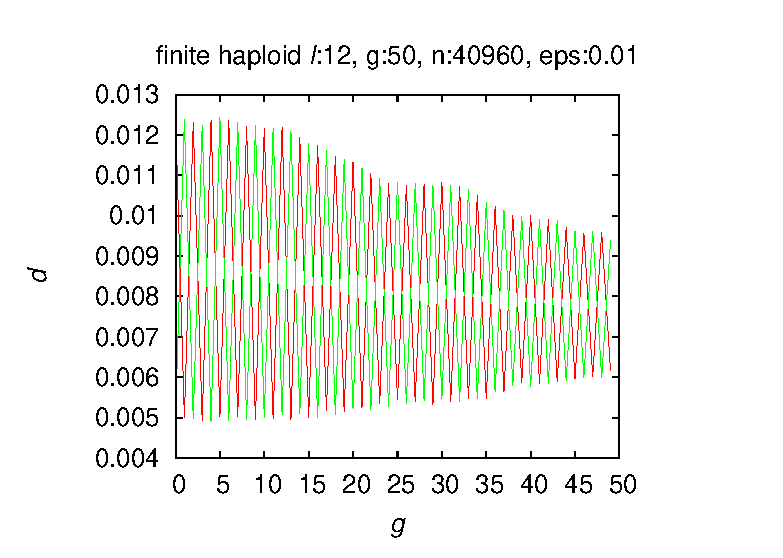
\includegraphics{figures/eps/vio/mu/b12/e0.01/n00040960_fin_hap_wovio.eps}}}\vspace{-1em} \hspace{-3em}%
\end{center}

\begin{center}
\subfloat{
\resizebox{8cm}{5cm}{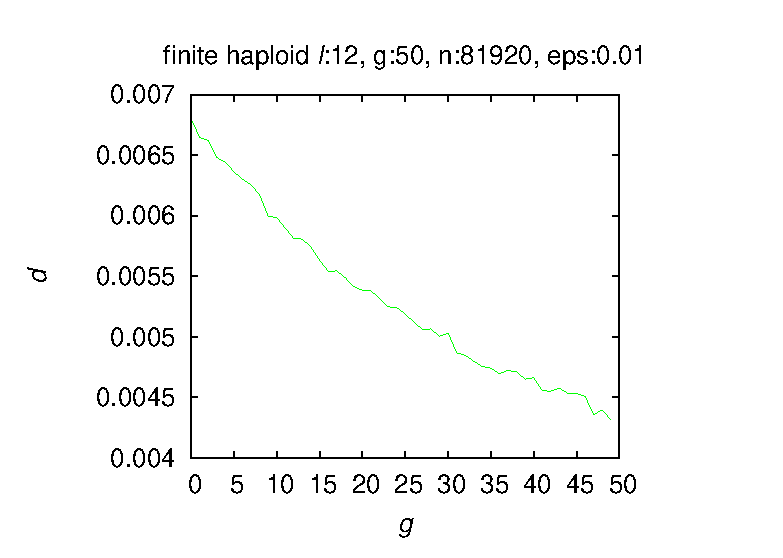
\includegraphics{figures/eps/vio/mu/b12/e0.01/n00081920_fin_hap.eps}}} \hspace{-3em}%
\subfloat{
\resizebox{8cm}{5cm}{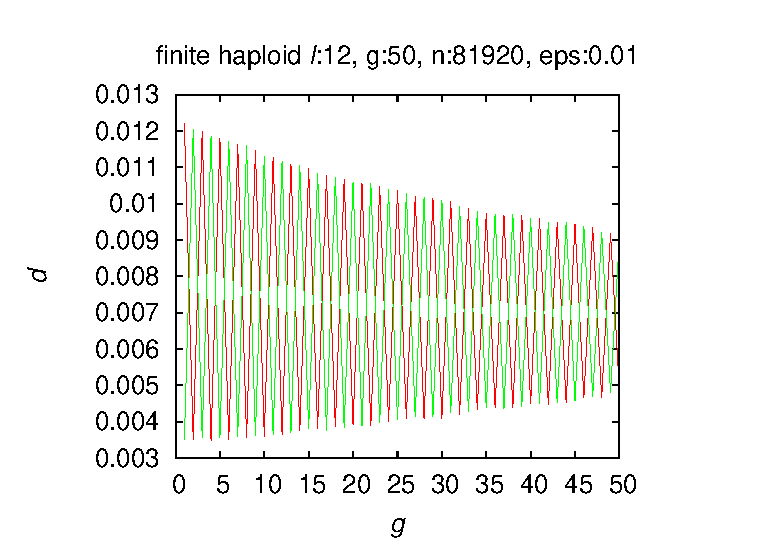
\includegraphics{figures/eps/vio/mu/b12/e0.01/n00081920_fin_hap_wovio.eps}}}\vspace{-1em} \hspace{-3em}%
\end{center}

\begin{center}
\subfloat{
\resizebox{8cm}{5cm}{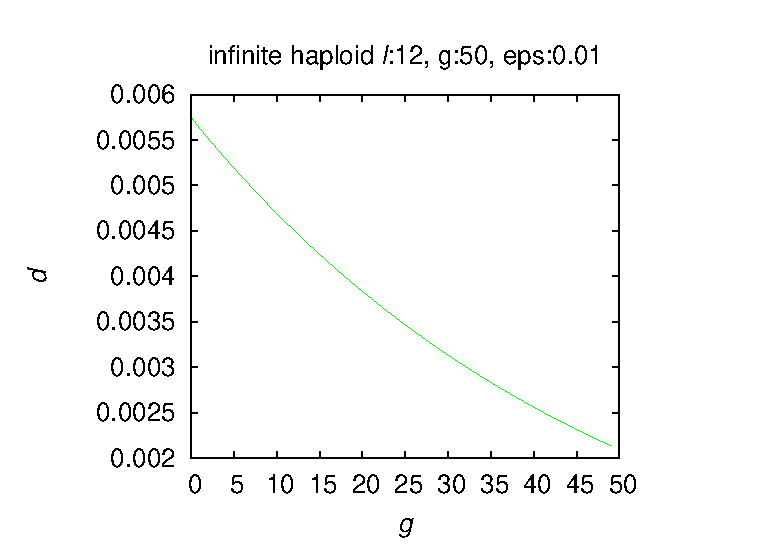
\includegraphics{figures/eps/vio/mu/b12/e0.01/inf_hap.eps}}}\hspace{-3em}%
\subfloat{
\resizebox{8cm}{5cm}{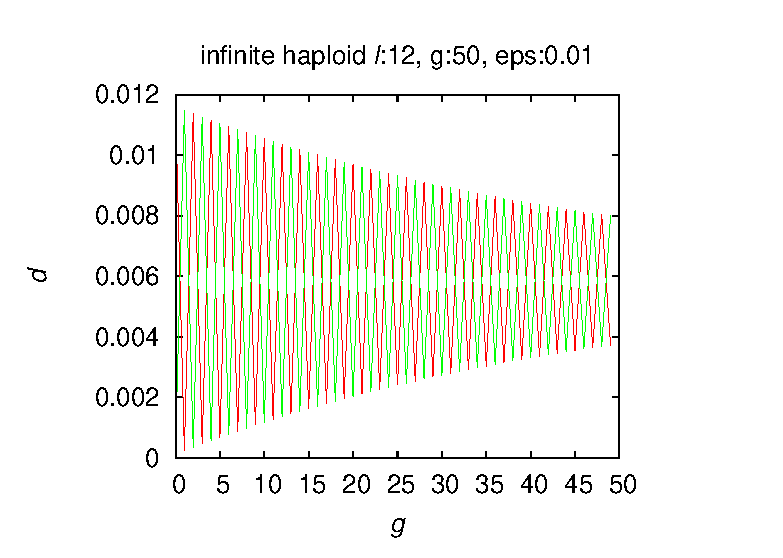
\includegraphics{figures/eps/vio/mu/b12/e0.01/inf_hap_wovio.eps}}}\vspace{-0.5em} \hspace{-3em}%
\caption{\textbf{Infinite and finite haploid population oscillation behavior in case of violation in $\bm{\mu}$ for genome length $\ell = 12$ and $\bm{\epsilon} = 0.01$:} 
  In left column, $d'$ is distance of finite population of size $n$ or infinite population to limit $\bm{z}^\ast$ for $g$ generations. In right column, $d$ is distance of finite population or infinite population to limits $\bm{p}^\ast$ and $\bm{q}^\ast$ without violation.}
\label{oscillation_12h_vio_mu_0.01}
\end{center}
\end{figure}

% l = 14

\begin{figure}[h]
\begin{center}
\subfloat{
\resizebox{8cm}{5cm}{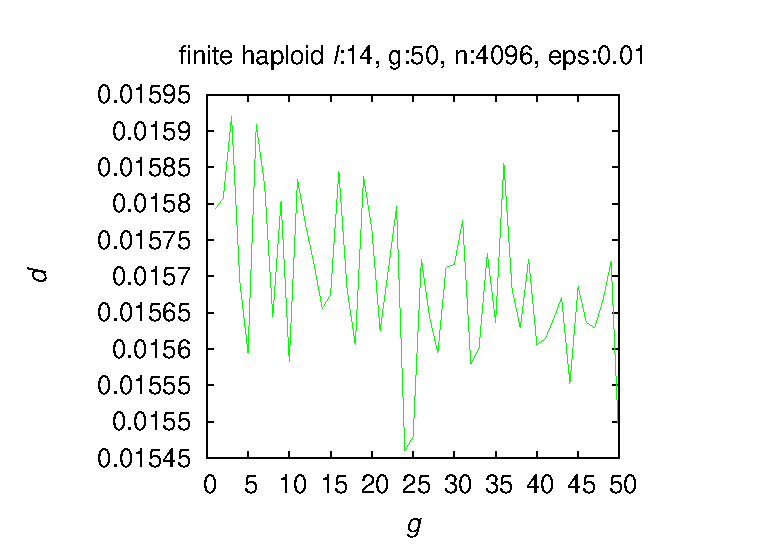
\includegraphics{figures/eps/vio/mu/b14/e0.01/n00004096_fin_hap.eps}}} \hspace{-3em}%
\subfloat{
\resizebox{8cm}{5cm}{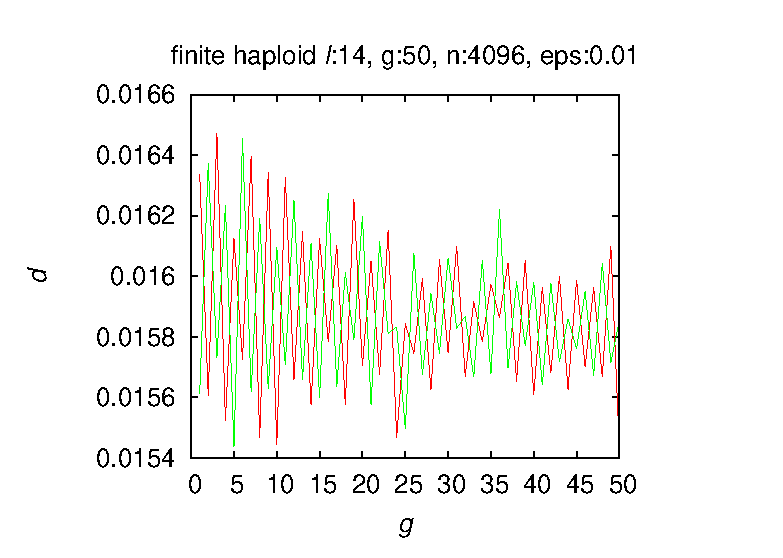
\includegraphics{figures/eps/vio/mu/b14/e0.01/n00004096_fin_hap_wovio.eps}}}\vspace{-1em} \hspace{-3em}%
\end{center}
\begin{center}
\subfloat{
\resizebox{8cm}{5cm}{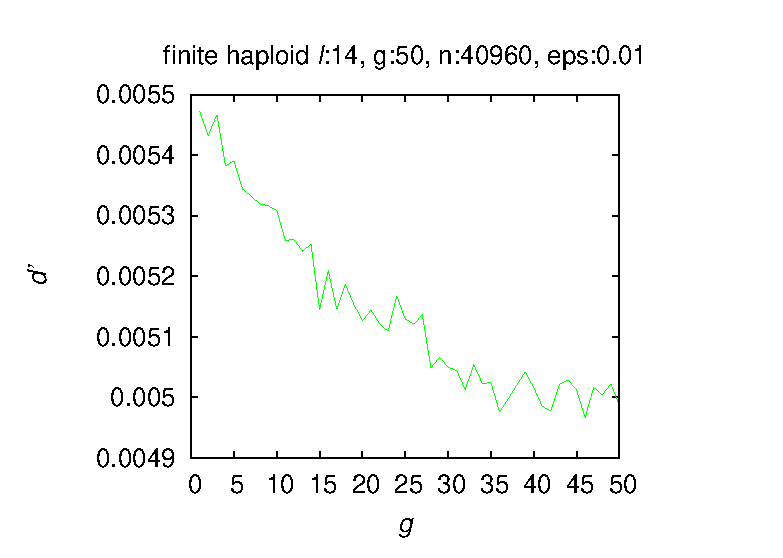
\includegraphics{figures/eps/vio/mu/b14/e0.01/n00040960_fin_hap.eps}}} \hspace{-3em}%
\subfloat{
\resizebox{8cm}{5cm}{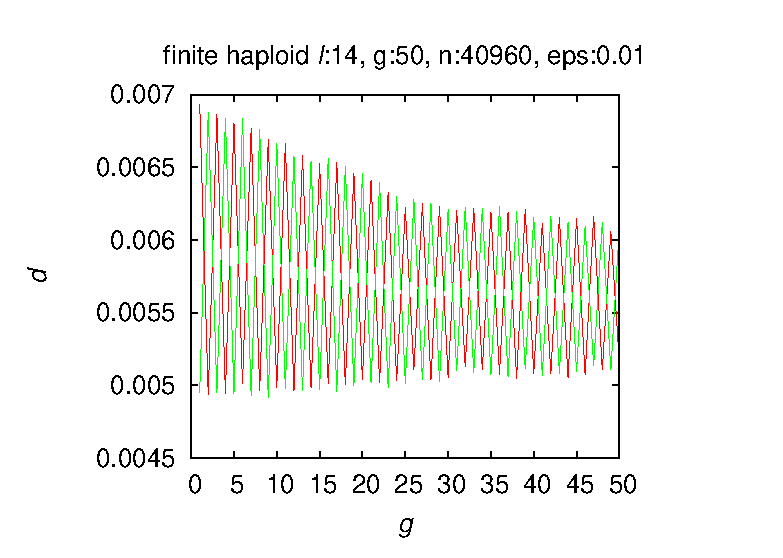
\includegraphics{figures/eps/vio/mu/b14/e0.01/n00040960_fin_hap_wovio.eps}}}\vspace{-1em} \hspace{-3em}%
\end{center}

\begin{center}
\subfloat{
\resizebox{8cm}{5cm}{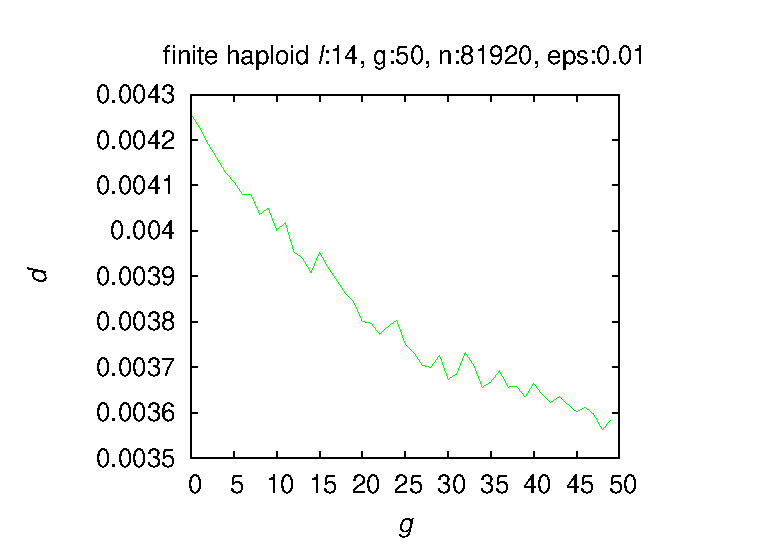
\includegraphics{figures/eps/vio/mu/b14/e0.01/n00081920_fin_hap.eps}}} \hspace{-3em}%
\subfloat{
\resizebox{8cm}{5cm}{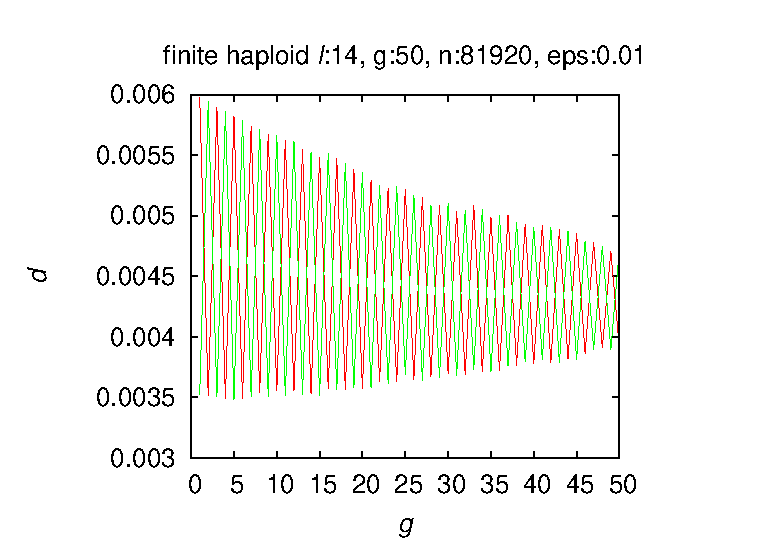
\includegraphics{figures/eps/vio/mu/b14/e0.01/n00081920_fin_hap_wovio.eps}}}\vspace{-1em} \hspace{-3em}%
\end{center}

\begin{center}
\subfloat{
\resizebox{8cm}{5cm}{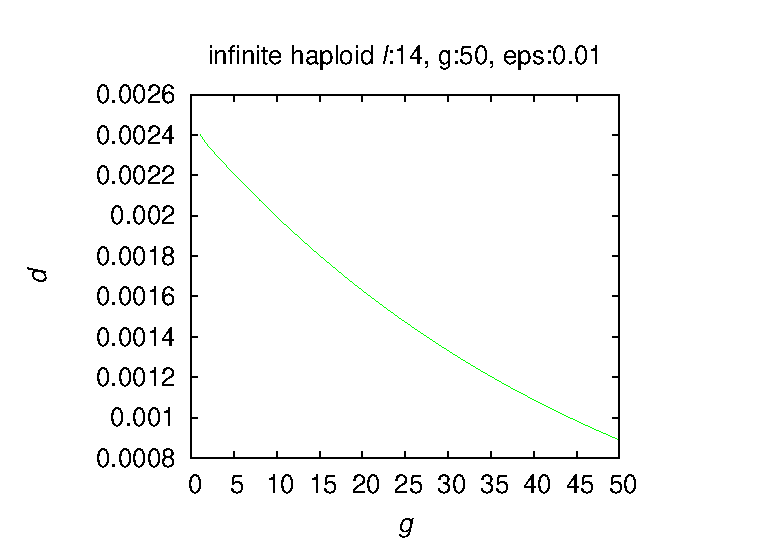
\includegraphics{figures/eps/vio/mu/b14/e0.01/inf_hap.eps}}}\hspace{-3em}%
\subfloat{
\resizebox{8cm}{5cm}{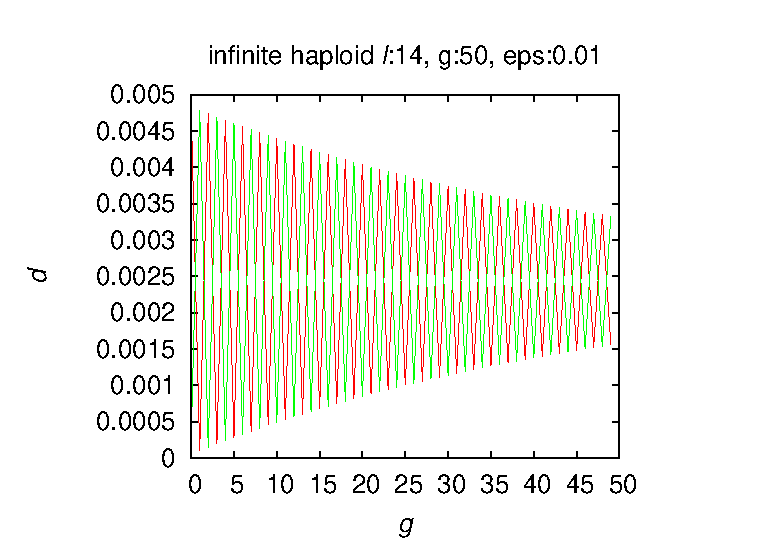
\includegraphics{figures/eps/vio/mu/b14/e0.01/inf_hap_wovio.eps}}}\vspace{-0.5em} \hspace{-3em}%
\caption{\textbf{Infinite and finite haploid population oscillation behavior in case of violation in $\bm{\mu}$ for genome length $\ell = 14$ and $\bm{\epsilon} = 0.01$:} 
  In left column, $d'$ is distance of finite population of size $n$ or infinite population to limit $\bm{z}^\ast$ for $g$ generations. In right column, $d$ is distance of finite population or infinite population to limits $\bm{p}^\ast$ and $\bm{q}^\ast$ without violation.}
\label{oscillation_14h_vio_mu_0.01}
\end{center}
\end{figure}

\clearpage

The right column in figures \ref{oscillation_8h_vio_mu_0.01} through \ref{oscillation_14h_vio_mu_0.01} 
shows distance of finite and infinite haploid populations to non-violation limits $\bm{p^\ast}$ and $\bm{q^\ast}$ with $\bm{\epsilon} \;=\; 0.01$. 
Those graphs indicate oscillating behavior of haploid population given violation. 
Both finite and infinite populations oscillate given violation. Oscillations are sharper. Since the value of $\bm{\epsilon}$ 
is small, damping of ripples is slow. The all zeros mask created in mutation distribution with $\bm{\epsilon} \;=\; 0.01$ have small 
probability of being used during mutation, and when it is not used, behavior should be consistent with the 
behavior without violation. Moreover, $\bm{\epsilon}$ is so small that 
infinite population oscillation does not die out completely in 50 generations.

The left column of figures \ref{oscillation_8h_vio_mu_0.01} through \ref{oscillation_14h_vio_mu_0.01} 
shows distance of finite and infinite haploid populations to limit $\bm{z^\ast}$ 
(limit with violation in mutation distribution $\bm{\mu}$) when $\bm{\epsilon} \;=\; 0.01$. 
The distance between finite population and limit $\bm{z}^\ast$ (limit with violation in $\bm{\mu}$ distribution) 
decreases as finite population size increases, 
and finite population shows behavior similar to infinite population behavior as finite population reach large number. 
Average distance data for haploid population in case of violation in $\bm{\mu}$ distribution 
with $\bm{\epsilon} \;=\; 0.01$ for different finite population size $N$ are tabulated in table \ref{distanceMuHapEps0.01}.

\begin{table}[ht]
\caption{\textbf{Distance measured for violation in $\bm{\mu}$ with $\bm{\epsilon} \;=\; 0.01$ for haploids:} $\ell$ is genome length, 
average distance between finite and infinite population is tabulated in the last three columns, and last row is expected single step distance.}
\centering
\begin{tabularx}{0.75\textwidth}{ c *{3}{X}}
\toprule
$\ell$ & $N = 4096$ & $N = 40960$ & $N = 81920$ \\
\midrule
8 & 0.0176	& 0.0094	& 0.0093 \\
10 & 0.0168	& 0.0088 	& 0.0077 \\ 
12 & 0.0161	& 0.0064 	& 0.0053 \\
14 & 0.0157	& 0.0051 	& 0.0038 \\ 
\midrule
$1/\sqrt{N}$ & 0.0156 & 0.0049 & 0.0035 \\
\bottomrule
\end{tabularx}
\label{distanceMuHapEps0.01}
\end{table}

From table \ref{distanceMuHapEps0.01}, average distance calculated for finite population size $4096$ is $0.0165$, 
for size $40960$ is $0.0074$ and for size $81920$ is $0.0065$. These results show average distance 
between finite population and limit $\bm{z^\ast}$ approach the expected single step distance 
between finite and infinite population. The distance decreased as $1/\sqrt{N}$. 
Also, the distance decreased as genome length $\ell$ increased for all sizes of finite haploid populations 
with $\bm{\epsilon} \;=\; 0.01$.


\subsection{Haploid Population $\mathtt{\sim}$ $\epsilon: 0.1$}
% l = 8

\begin{figure}[h]
\begin{center}
\subfloat{
\resizebox{8cm}{5cm}{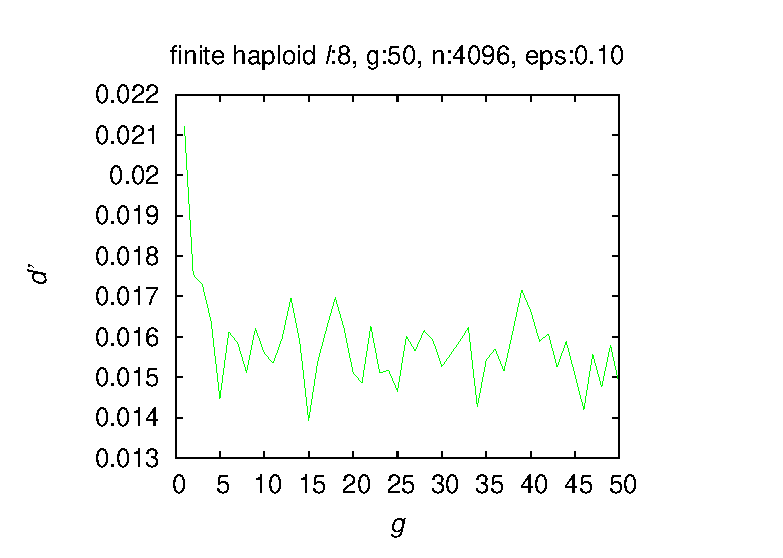
\includegraphics{figures/eps/vio/mu/b8/e0.1/n00004096_fin_hap.eps}}} \hspace{-3em}%
\subfloat{
\resizebox{8cm}{5cm}{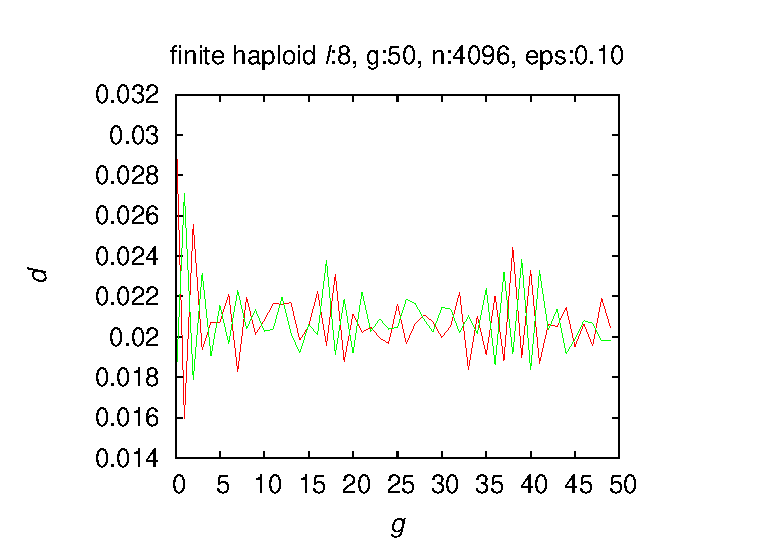
\includegraphics{figures/eps/vio/mu/b8/e0.1/n00004096_fin_hap_wovio.eps}}}\vspace{-1em} \hspace{-3em}%
\end{center}
\begin{center}
\subfloat{
\resizebox{8cm}{5cm}{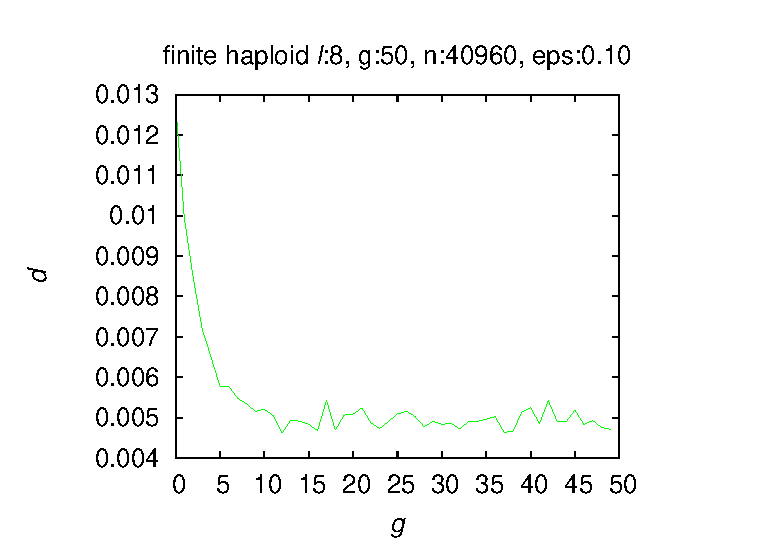
\includegraphics{figures/eps/vio/mu/b8/e0.1/n00040960_fin_hap.eps}}} \hspace{-3em}%
\subfloat{
\resizebox{8cm}{5cm}{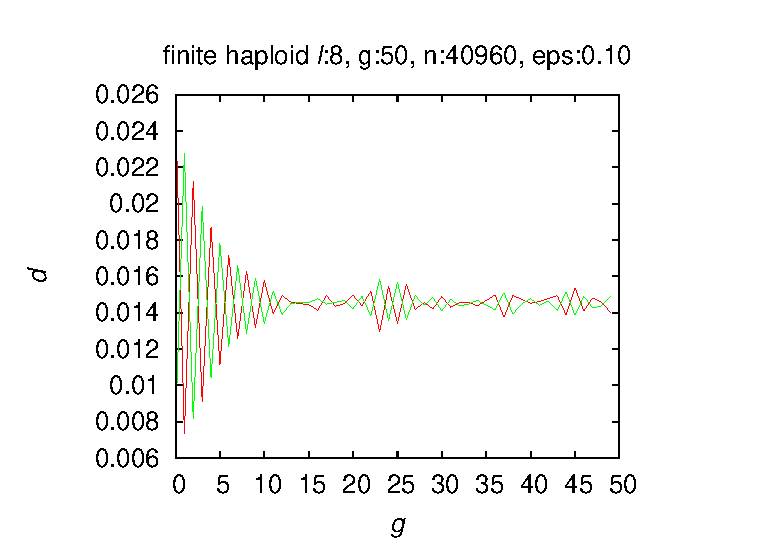
\includegraphics{figures/eps/vio/mu/b8/e0.1/n00040960_fin_hap_wovio.eps}}}\vspace{-1em} \hspace{-3em}%
\end{center}

\begin{center}
\subfloat{
\resizebox{8cm}{5cm}{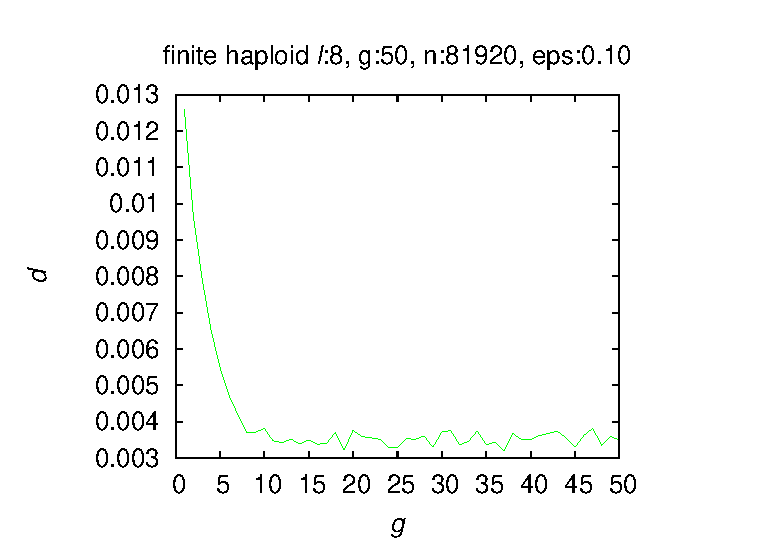
\includegraphics{figures/eps/vio/mu/b8/e0.1/n00081920_fin_hap.eps}}} \hspace{-3em}%
\subfloat{
\resizebox{8cm}{5cm}{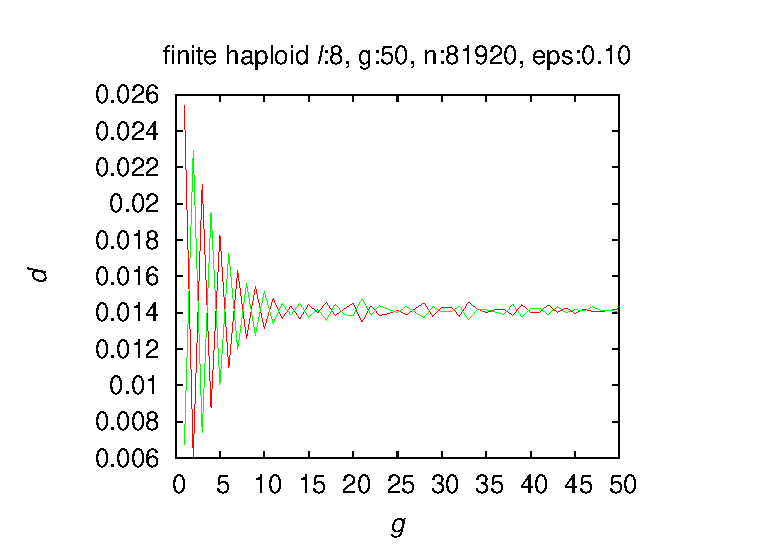
\includegraphics{figures/eps/vio/mu/b8/e0.1/n00081920_fin_hap_wovio.eps}}}\vspace{-1em} \hspace{-3em}%
\end{center}

\begin{center}
\subfloat{
\resizebox{8cm}{5cm}{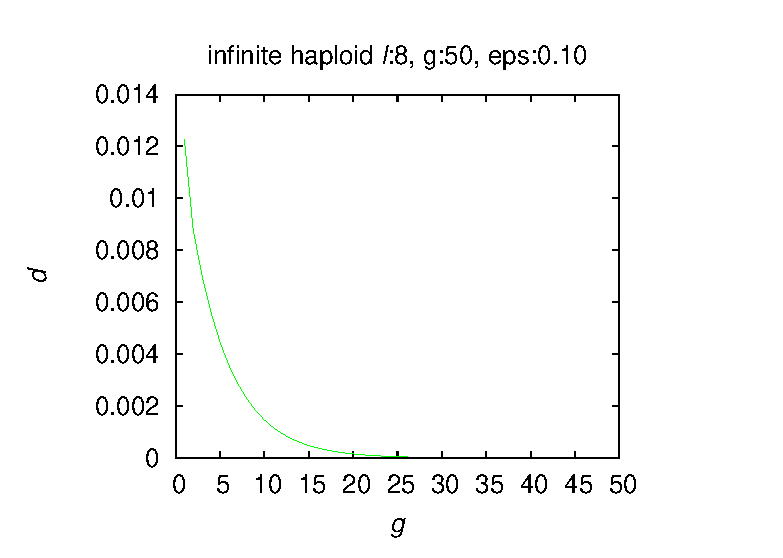
\includegraphics{figures/eps/vio/mu/b8/e0.1/inf_hap.eps}}}\hspace{-3em}%
\subfloat{
\resizebox{8cm}{5cm}{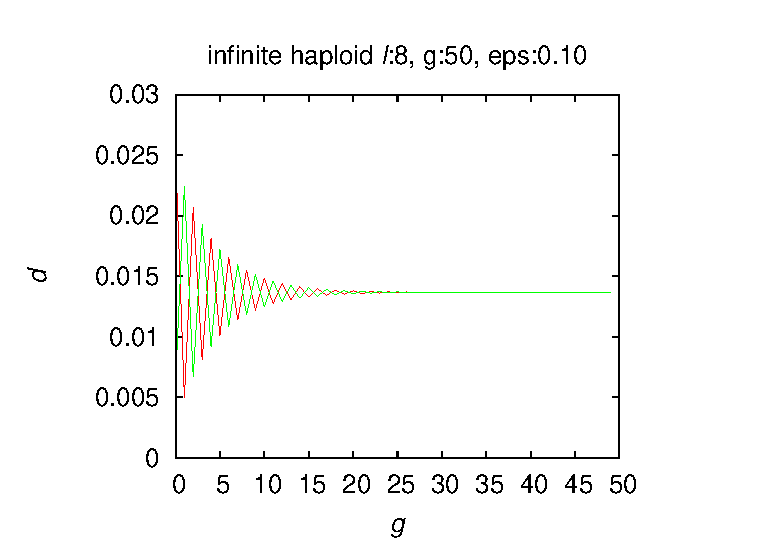
\includegraphics{figures/eps/vio/mu/b8/e0.1/inf_hap_wovio.eps}}}\vspace{-0.5em} \hspace{-3em}%


\caption[\textbf{Infinite and finite haploid population oscillation behavior in case of violation in $\bm{\mu}$ for genome length $\ell = 8$ and $\bm{\epsilon} = 0.1$}]{\textbf{Infinite and finite haploid population oscillation behavior in case of violation in $\bm{\mu}$ for genome length $\ell = 8$ and $\bm{\epsilon} = 0.1$:} 
  In left column, $d'$ is distance of finite population of size $n$ or infinite population to limit $\bm{z}^\ast$ for $g$ generations. In right column, $d$ is distance of finite population or infinite population to limits $\bm{p}^\ast$ and $\bm{q}^\ast$ without violation.}
\label{oscillation_8h_vio_mu_0.1}
\end{center}
\end{figure}

% l = 10

\begin{figure}[h]
\begin{center}
\subfloat{
\resizebox{8cm}{5cm}{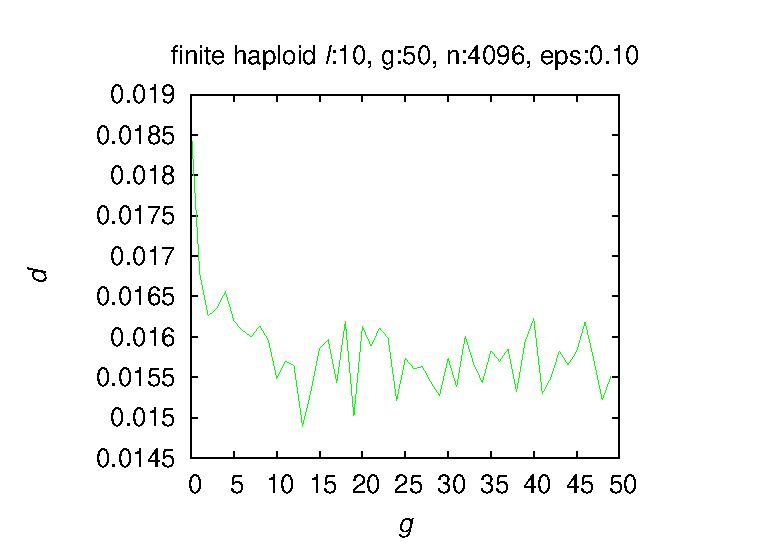
\includegraphics{figures/eps/vio/mu/b10/e0.1/n00004096_fin_hap.eps}}} \hspace{-3em}%
\subfloat{
\resizebox{8cm}{5cm}{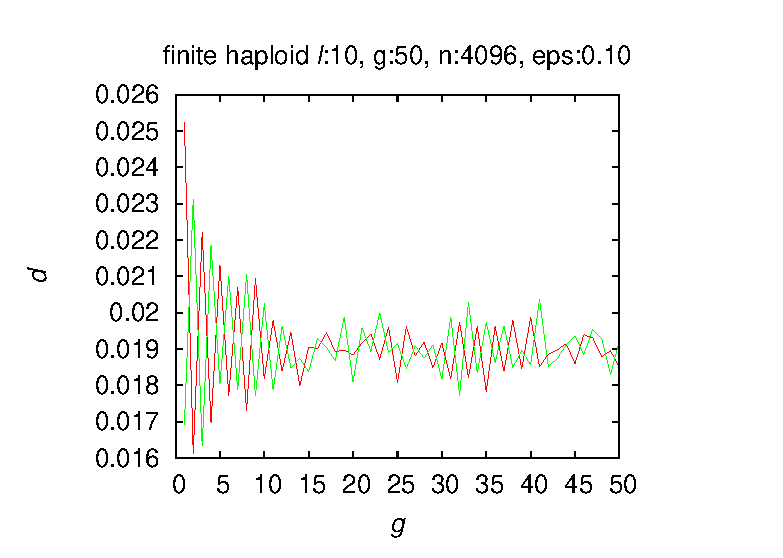
\includegraphics{figures/eps/vio/mu/b10/e0.1/n00004096_fin_hap_wovio.eps}}}\vspace{-1em} \hspace{-3em}%
\end{center}
\begin{center}
\subfloat{
\resizebox{8cm}{5cm}{\includegraphics{figures/eps/vio/mu/b10/e0.1/n00040960_fin_hap.eps}}} \hspace{-3em}%
\subfloat{
\resizebox{8cm}{5cm}{\includegraphics{figures/eps/vio/mu/b10/e0.1/n00040960_fin_hap_wovio.eps}}}\vspace{-1em} \hspace{-3em}%
\end{center}

\begin{center}
\subfloat{
\resizebox{8cm}{5cm}{\includegraphics{figures/eps/vio/mu/b10/e0.1/n00081920_fin_hap.eps}}} \hspace{-3em}%
\subfloat{
\resizebox{8cm}{5cm}{\includegraphics{figures/eps/vio/mu/b10/e0.1/n00081920_fin_hap_wovio.eps}}}\vspace{-1em} \hspace{-3em}%
\end{center}

\begin{center}
\subfloat{
\resizebox{8cm}{5cm}{\includegraphics{figures/eps/vio/mu/b10/e0.1/inf_hap.eps}}}\hspace{-3em}%
\subfloat{
\resizebox{8cm}{5cm}{\includegraphics{figures/eps/vio/mu/b10/e0.1/inf_hap_wovio.eps}}}\vspace{-0.5em} \hspace{-3em}%


\caption[\textbf{Infinite and finite haploid population oscillation behavior in case of violation in $\bm{\mu}$ for genome length $\ell = 10$ and $\bm{\epsilon} = 0.1$}]{\textbf{Infinite and finite haploid population oscillation behavior in case of violation in $\bm{\mu}$ for genome length $\ell = 10$ and $\bm{\epsilon} = 0.1$:} 
  In left column, $d'$ is distance of finite population of size $n$ or infinite population to limit $\bm{z}^\ast$ for $g$ generations. In right column, $d$ is distance of finite population or infinite population to limits $\bm{p}^\ast$ and $\bm{q}^\ast$ without violation.}
\label{oscillation_10h_vio_mu_0.1}
\end{center}
\end{figure}

% l = 12

\begin{figure}[h]
\begin{center}
\subfloat{
\resizebox{8cm}{5cm}{\includegraphics{figures/eps/vio/mu/b12/e0.1/n00004096_fin_hap.eps}}} \hspace{-3em}%
\subfloat{
\resizebox{8cm}{5cm}{\includegraphics{figures/eps/vio/mu/b12/e0.1/n00004096_fin_hap_wovio.eps}}}\vspace{-1em} \hspace{-3em}%
\end{center}
\begin{center}
\subfloat{
\resizebox{8cm}{5cm}{\includegraphics{figures/eps/vio/mu/b12/e0.1/n00040960_fin_hap.eps}}} \hspace{-3em}%
\subfloat{
\resizebox{8cm}{5cm}{\includegraphics{figures/eps/vio/mu/b12/e0.1/n00040960_fin_hap_wovio.eps}}}\vspace{-1em} \hspace{-3em}%
\end{center}

\begin{center}
\subfloat{
\resizebox{8cm}{5cm}{\includegraphics{figures/eps/vio/mu/b12/e0.1/n00081920_fin_hap.eps}}} \hspace{-3em}%
\subfloat{
\resizebox{8cm}{5cm}{\includegraphics{figures/eps/vio/mu/b12/e0.1/n00081920_fin_hap_wovio.eps}}}\vspace{-1em} \hspace{-3em}%
\end{center}

\begin{center}
\subfloat{
\resizebox{8cm}{5cm}{\includegraphics{figures/eps/vio/mu/b12/e0.1/inf_hap.eps}}}\hspace{-3em}%
\subfloat{
\resizebox{8cm}{5cm}{\includegraphics{figures/eps/vio/mu/b12/e0.1/inf_hap_wovio.eps}}}\vspace{-0.5em} \hspace{-3em}%


\caption[\textbf{Infinite and finite haploid population oscillation behavior in case of violation in $\bm{\mu}$ for genome length $\ell = 12$ and $\bm{\epsilon} = 0.1$}]{\textbf{Infinite and finite haploid population oscillation behavior in case of violation in $\bm{\mu}$ for genome length $\ell = 12$ and $\bm{\epsilon} = 0.1$:} 
  In left column, $d'$ is distance of finite population of size $n$ or infinite population to limit $\bm{z}^\ast$ for $g$ generations. In right column, $d$ is distance of finite population or infinite population to limits $\bm{p}^\ast$ and $\bm{q}^\ast$ without violation.}
\label{oscillation_12h_vio_mu_0.1}
\end{center}
\end{figure}

% l = 14

\begin{figure}[h]
\begin{center}
\subfloat{
\resizebox{8cm}{5cm}{\includegraphics{figures/eps/vio/mu/b14/e0.1/n00004096_fin_hap.eps}}} \hspace{-3em}%
\subfloat{
\resizebox{8cm}{5cm}{\includegraphics{figures/eps/vio/mu/b14/e0.1/n00004096_fin_hap_wovio.eps}}}\vspace{-1em} \hspace{-3em}%
\end{center}
\begin{center}
\subfloat{
\resizebox{8cm}{5cm}{\includegraphics{figures/eps/vio/mu/b14/e0.1/n00040960_fin_hap.eps}}} \hspace{-3em}%
\subfloat{
\resizebox{8cm}{5cm}{\includegraphics{figures/eps/vio/mu/b14/e0.1/n00040960_fin_hap_wovio.eps}}}\vspace{-1em} \hspace{-3em}%
\end{center}

\begin{center}
\subfloat{
\resizebox{8cm}{5cm}{\includegraphics{figures/eps/vio/mu/b14/e0.1/n00081920_fin_hap.eps}}} \hspace{-3em}%
\subfloat{
\resizebox{8cm}{5cm}{\includegraphics{figures/eps/vio/mu/b14/e0.1/n00081920_fin_hap_wovio.eps}}}\vspace{-1em} \hspace{-3em}%
\end{center}

\begin{center}
\subfloat{
\resizebox{8cm}{5cm}{\includegraphics{figures/eps/vio/mu/b14/e0.1/inf_hap.eps}}}\hspace{-3em}%
\subfloat{
\resizebox{8cm}{5cm}{\includegraphics{figures/eps/vio/mu/b14/e0.1/inf_hap_wovio.eps}}}\vspace{-0.5em} \hspace{-3em}%


\caption[\textbf{Infinite and finite haploid population oscillation behavior in case of violation in $\bm{\mu}$ for genome length $\ell = 14$ and $\bm{\epsilon} = 0.1$}]{\textbf{Infinite and finite haploid population oscillation behavior in case of violation in $\bm{\mu}$ for genome length $\ell = 14$ and $\bm{\epsilon} = 0.1$:} 
  In left column, $d'$ is distance of finite population of size $n$ or infinite population to limit $\bm{z}^\ast$ for $g$ generations. In right column, $d$ is distance of finite population or infinite population to limits $\bm{p}^\ast$ and $\bm{q}^\ast$ without violation.}
\label{oscillation_14h_vio_mu_0.1}
\end{center}
\end{figure}

\clearpage

The right column in figures \ref{oscillation_8h_vio_mu_0.1} through \ref{oscillation_14h_vio_mu_0.1} 
shows distance of finite and infinite haploid populations to non-violation limits $\bm{p^\ast}$ and $\bm{q^\ast}$ with $\bm{\epsilon} \;=\; 0.1$. 
Those graphs indicate oscillating behavior of haploid population given violation. 
Both finite and infinite populations oscillate given violation, and oscillations amplitudes decreases with time. 
However, for $\bm{\epsilon} \;=\; 0.1$, oscillations in infinite populations die out quickly, 
but oscillations in finite populations does not die out completely. Rate of damping of ripples with $\bm{\epsilon} \;=\; 0.1$ is  
larger than with $\bm{\epsilon} \;=\; 0.01$. The all zeroz mask created in mutation distribution with $\bm{\epsilon} \;=\; 0.1$ have small  
probability of being used during mutation making it unlikely for oscillation in finite populations to die out quickly.

The left column of figures \ref{oscillation_8h_vio_mu_0.1} through \ref{oscillation_14h_vio_mu_0.1} 
shows distance of finite and infinite haploid populations to limit $\bm{z^\ast}$ 
(limit with violation in mutation distribution $\bm{\mu}$) when $\bm{\epsilon} \;=\; 0.1$. 
The distance between finite population and limit $\bm{z}^\ast$ (limit with violation in $\bm{\mu}$ distribution) 
decreases as finite population size increases, 
and finite population shows behavior similar to infinite population behavior as finite population size grows. 
Average distance data for haploid population in case of violation in $\bm{\mu}$ distribution 
with $\bm{\epsilon} \;=\; 0.1$ for different finite population size $N$ is tabulated in table \ref{distanceMuHapEps0.1}.

\begin{table}[ht]
\caption[\textbf{Distance measured for violation in $\bm{\mu}$ with $\bm{\epsilon} \;=\; 0.1$ for haploids}]{\textbf{Distance measured for violation in $\bm{\mu}$ with $\bm{\epsilon} \;=\; 0.1$ for haploids:} $\ell$ is genome length, 
average distance between finite and infinite population is tabulated in the last three columns, and last row is expected single step distance.}
\centering
\begin{tabularx}{0.75\textwidth}{ c *{3}{X}}
\toprule
$\ell$ & $N = 4096$ & $N = 40960$ & $N = 81920$ \\
\midrule
8 & 0.0158	& 0.0054 	& 0.0041 \\
10 & 0.0158	& 0.0053 	& 0.0039 \\	
12 & 0.0157	& 0.0051 	& 0.0036 \\	
14 & 0.0156	& 0.0050 	& 0.0035 \\
\midrule
$1/\sqrt{N}$ & 0.0156 & 0.0049 & 0.0035 \\
\bottomrule
\end{tabularx}
\label{distanceMuHapEps0.1}
\end{table}

The results in Table \ref{distanceMuHapEps0.1} show average distance 
between finite population and limit $\bm{z^\ast}$ approach the expected single step distance 
between finite and infinite population. The distance decreased as $1/\sqrt{N}$. 
Also, the distance decreased as genome length $\ell$ increased for all sizes of finite haploid populations 
with $\bm{\epsilon} \;=\; 0.1$.

\subsection{Haploid Population $\mathtt{\sim}$ $\epsilon: 0.5$}
% l = 8
% \mbox{}\\[-0.75in]
\begin{figure}[!b]
\begin{center}
\subfloat{
\resizebox{8cm}{4.5cm}{\includegraphics{figures/eps/vio/mu/b8/e0.5/n00004096_fin_hap.eps}}} \hspace{-3em}%
\subfloat{
\resizebox{8cm}{4.5cm}{\includegraphics{figures/eps/vio/mu/b8/e0.5/n00004096_fin_hap_wovio.eps}}}\vspace{-1em} \hspace{-3em}%
\end{center}
\begin{center}
\subfloat{
\resizebox{8cm}{4.5cm}{\includegraphics{figures/eps/vio/mu/b8/e0.5/n00040960_fin_hap.eps}}} \hspace{-3em}%
\subfloat{
\resizebox{8cm}{4.5cm}{\includegraphics{figures/eps/vio/mu/b8/e0.5/n00040960_fin_hap_wovio.eps}}}\vspace{-1em} \hspace{-3em}%
\end{center}

\begin{center}
\subfloat{
\resizebox{8cm}{4.5cm}{\includegraphics{figures/eps/vio/mu/b8/e0.5/n00081920_fin_hap.eps}}} \hspace{-3em}%
\subfloat{
\resizebox{8cm}{4.5cm}{\includegraphics{figures/eps/vio/mu/b8/e0.5/n00081920_fin_hap_wovio.eps}}}\vspace{-1em} \hspace{-3em}%
\end{center}

\begin{center}
\subfloat{
\resizebox{8cm}{4.5cm}{\includegraphics{figures/eps/vio/mu/b8/e0.5/inf_hap.eps}}}\hspace{-3em}%
\subfloat{
\resizebox{8cm}{4.5cm}{\includegraphics{figures/eps/vio/mu/b8/e0.5/inf_hap_wovio.eps}}}\vspace{-0.5em} \hspace{-3em}%


\caption[\textbf{Infinite and finite haploid population behavior in case of violation in $\bm{\mu}$ for genome length $\ell = 8$ and $\bm{\epsilon} = 0.5$}]
{\textbf{Infinite and finite haploid population behavior for $\bm{\mu}$ violation and $\ell = 8$ and $\bm{\epsilon} = 0.5$:} 
  In left column, $d'$ is distance of finite or infinite population to limit $\bm{z}^\ast$ for $g$ generations. 
  In right column, $d$ is distance of finite or infinite population to limits $\bm{p}^\ast$ and $\bm{q}^\ast$. Green line is distance to $\bm{p*}$ and red line is distance to $\bm{q*}$.}
  \label{oscillation_8h_vio_mu_0.5}
\end{center}
\end{figure}

% l = 10

\begin{figure}[h]
\begin{center}
\subfloat{
\resizebox{8cm}{4.5cm}{\includegraphics{figures/eps/vio/mu/b10/e0.5/n00004096_fin_hap.eps}}} \hspace{-3em}%
\subfloat{
\resizebox{8cm}{4.5cm}{\includegraphics{figures/eps/vio/mu/b10/e0.5/n00004096_fin_hap_wovio.eps}}}\vspace{-1em} \hspace{-3em}%
\end{center}
\begin{center}
\subfloat{
\resizebox{8cm}{4.5cm}{\includegraphics{figures/eps/vio/mu/b10/e0.5/n00040960_fin_hap.eps}}} \hspace{-3em}%
\subfloat{
\resizebox{8cm}{4.5cm}{\includegraphics{figures/eps/vio/mu/b10/e0.5/n00040960_fin_hap_wovio.eps}}}\vspace{-1em} \hspace{-3em}%
\end{center}

\begin{center}
\subfloat{
\resizebox{8cm}{4.5cm}{\includegraphics{figures/eps/vio/mu/b10/e0.5/n00081920_fin_hap.eps}}} \hspace{-3em}%
\subfloat{
\resizebox{8cm}{4.5cm}{\includegraphics{figures/eps/vio/mu/b10/e0.5/n00081920_fin_hap_wovio.eps}}}\vspace{-1em} \hspace{-3em}%
\end{center}

\begin{center}
\subfloat{
\resizebox{8cm}{4.5cm}{\includegraphics{figures/eps/vio/mu/b10/e0.5/inf_hap.eps}}}\hspace{-3em}%
\subfloat{
\resizebox{8cm}{4.5cm}{\includegraphics{figures/eps/vio/mu/b10/e0.5/inf_hap_wovio.eps}}}\vspace{-0.5em} \hspace{-3em}%


\caption[\textbf{Infinite and finite haploid population behavior $\bm{\mu}$ for violation, genome length $\ell = 10$ and $\bm{\epsilon} = 0.5$}]{\textbf{Infinite and finite haploid population behavior $\bm{\mu}$ for violation, genome length $\ell = 10$ and $\bm{\epsilon} = 0.5$:} 
  In left column, $d'$ is distance of finite or infinite population to limit $\bm{z}^\ast$ for $g$ generations. In right column, $d$ is distance of finite or infinite population to limits $\bm{p}^\ast$ and $\bm{q}^\ast$. Green line is distance to $\bm{p*}$ and red line is distance to $\bm{q*}$.}
\label{oscillation_10h_vio_mu_0.5}
\end{center}
\end{figure}

% l = 12

\begin{figure}[h]
\begin{center}
\subfloat{
\resizebox{8cm}{4.5cm}{\includegraphics{figures/eps/vio/mu/b12/e0.5/n00004096_fin_hap.eps}}} \hspace{-3em}%
\subfloat{
\resizebox{8cm}{4.5cm}{\includegraphics{figures/eps/vio/mu/b12/e0.5/n00004096_fin_hap_wovio.eps}}}\vspace{-1em} \hspace{-3em}%
\end{center}
\begin{center}
\subfloat{
\resizebox{8cm}{4.5cm}{\includegraphics{figures/eps/vio/mu/b12/e0.5/n00040960_fin_hap.eps}}} \hspace{-3em}%
\subfloat{
\resizebox{8cm}{4.5cm}{\includegraphics{figures/eps/vio/mu/b12/e0.5/n00040960_fin_hap_wovio.eps}}}\vspace{-1em} \hspace{-3em}%
\end{center}

\begin{center}
\subfloat{
\resizebox{8cm}{4.5cm}{\includegraphics{figures/eps/vio/mu/b12/e0.5/n00081920_fin_hap.eps}}} \hspace{-3em}%
\subfloat{
\resizebox{8cm}{4.5cm}{\includegraphics{figures/eps/vio/mu/b12/e0.5/n00081920_fin_hap_wovio.eps}}}\vspace{-1em} \hspace{-3em}%
\end{center}

\begin{center}
\subfloat{
\resizebox{8cm}{4.5cm}{\includegraphics{figures/eps/vio/mu/b12/e0.5/inf_hap.eps}}}\hspace{-3em}%
\subfloat{
\resizebox{8cm}{4.5cm}{\includegraphics{figures/eps/vio/mu/b12/e0.5/inf_hap_wovio.eps}}}\vspace{-0.5em} \hspace{-3em}%


\caption[\textbf{Infinite and finite haploid population behavior $\bm{\mu}$ for violation, genome length $\ell = 12$ and $\bm{\epsilon} = 0.5$}]{\textbf{Infinite and finite haploid population behavior $\bm{\mu}$ for violation, genome length $\ell = 12$ and $\bm{\epsilon} = 0.5$:} 
  In left column, $d'$ is distance of finite or infinite population to limit $\bm{z}^\ast$ for $g$ generations. In right column, $d$ is distance of finite or infinite population to limits $\bm{p}^\ast$ and $\bm{q}^\ast$. Green line is distance to $\bm{p*}$ and red line is distance to $\bm{q*}$.}
\label{oscillation_12h_vio_mu_0.5}
\end{center}
\end{figure}

% l = 14

\begin{figure}[h]
\begin{center}
\subfloat{
\resizebox{8cm}{4.5cm}{\includegraphics{figures/eps/vio/mu/b14/e0.5/n00004096_fin_hap.eps}}} \hspace{-3em}%
\subfloat{
\resizebox{8cm}{4.5cm}{\includegraphics{figures/eps/vio/mu/b14/e0.5/n00004096_fin_hap_wovio.eps}}}\vspace{-1em} \hspace{-3em}%
\end{center}
\begin{center}
\subfloat{
\resizebox{8cm}{4.5cm}{\includegraphics{figures/eps/vio/mu/b14/e0.5/n00040960_fin_hap.eps}}} \hspace{-3em}%
\subfloat{
\resizebox{8cm}{4.5cm}{\includegraphics{figures/eps/vio/mu/b14/e0.5/n00040960_fin_hap_wovio.eps}}}\vspace{-1em} \hspace{-3em}%
\end{center}

\begin{center}
\subfloat{
\resizebox{8cm}{4.5cm}{\includegraphics{figures/eps/vio/mu/b14/e0.5/n00081920_fin_hap.eps}}} \hspace{-3em}%
\subfloat{
\resizebox{8cm}{4.5cm}{\includegraphics{figures/eps/vio/mu/b14/e0.5/n00081920_fin_hap_wovio.eps}}}\vspace{-1em} \hspace{-3em}%
\end{center}

\begin{center}
\subfloat{
\resizebox{8cm}{4.5cm}{\includegraphics{figures/eps/vio/mu/b14/e0.5/inf_hap.eps}}}\hspace{-3em}%
\subfloat{
\resizebox{8cm}{4.5cm}{\includegraphics{figures/eps/vio/mu/b14/e0.5/inf_hap_wovio.eps}}}\vspace{-0.5em} \hspace{-3em}%

\caption[\textbf{Infinite and finite haploid population behavior $\bm{\mu}$ for violation, genome length $\ell = 14$ and $\bm{\epsilon} = 0.5$}]{\textbf{Infinite and finite haploid population behavior $\bm{\mu}$ for violation, genome length $\ell = 14$ and $\bm{\epsilon} = 0.5$:} 
  In left column, $d'$ is distance of finite or infinite population to limit $\bm{z}^\ast$ for $g$ generations. In right column, $d$ is distance of finite or infinite population to limits $\bm{p}^\ast$ and $\bm{q}^\ast$. Green line is distance to $\bm{p*}$ and red line is distance to $\bm{q*}$.}
\label{oscillation_14h_vio_mu_0.5}
\end{center}
\end{figure}

% \clearpage
The right column in figures \ref{oscillation_8h_vio_mu_0.5} through \ref{oscillation_14h_vio_mu_0.5} 
shows distance of finite and infinite haploid populations to non-violation limits $\bm{p^\ast}$ and $\bm{q^\ast}$ with $\bm{\epsilon} \;=\; 0.5$. 
The graphs indicate oscillating behavior of haploid population given violation. 
Neither finite nor infinite populations show noticable oscillation given violation. 
The all zeros mask created in mutation distribution with $\bm{\epsilon} \;=\; 0.5$ has a large probability 
of being used during mutation, so oscillation decreased signficantly.

The left column of figures \ref{oscillation_8h_vio_mu_0.5} through \ref{oscillation_14h_vio_mu_0.5} 
shows distance of finite and infinite haploid populations to limit $\bm{z^\ast}$ 
(limit with violation in mutation distribution $\bm{\mu}$) when $\bm{\epsilon} \;=\; 0.5$. 
The distance decreases as finite population size increases, 
and finite population shows behavior similar to infinite population behavior as finite population size grows. 
Average distance data for haploid population in case of violation in $\bm{\mu}$ distribution 
with $\bm{\epsilon} \;=\; 0.5$ for different finite population size $N$ are tabulated in table \ref{distanceMuHapEps0.5}.

\clearpage
\begin{table}[h]
\caption[\textbf{Distance measured for violation in $\bm{\mu}$ with $\bm{\epsilon} \;=\; 0.5$ for haploids}]{\textbf{Distance measured for violation in $\bm{\mu}$ with $\bm{\epsilon} \;=\; 0.5$ for haploids:} $\ell$ is genome length, 
average distance between finite and infinite population is tabulated in the last three columns, and last row is expected single step distance.}
\centering
\begin{tabularx}{0.75\textwidth}{ c *{3}{X}}
\toprule
$\ell$ & $N = 4096$ & $N = 40960$ & $N = 81920$ \\
\midrule
8 & 0.0161	&  0.0056	& 0.0042 \\
10 & 0.0161	&  0.0055	& 0.0040 \\
12 & 0.0157	&  0.0051	& 0.0036 \\
14 & 0.0157	&  0.0051	& 0.0036 \\
\midrule
$1/\sqrt{N}$ & 0.0156 & 0.0049 & 0.0035 \\
\bottomrule
\end{tabularx}
\label{distanceMuHapEps0.5}
\end{table}
 
Table \ref{distanceMuHapEps0.5} shows that the average distance 
between finite population and infinite population decreases with increasing string length, 
approaching the expected single step distance $1/\sqrt{N}$. 

\subsection{Diploid Population $\mathtt{\sim}$ $\epsilon: 0.01$}
% l = 8

\begin{figure}[H]
\begin{center}
\subfloat{
\resizebox{8cm}{5cm}{\includegraphics{figures/eps/vio/mu/b8/e0.01/n00004096_fin_dip.eps}}}\hspace{-3em}%
\subfloat{
\resizebox{8cm}{5cm}{\includegraphics{figures/eps/vio/mu/b8/e0.01/n00004096_fin_dip_wovio.eps}}}\vspace{-1em}  \hspace{-3em}%
\end{center}
\begin{center}
\subfloat{
\resizebox{8cm}{5cm}{\includegraphics{figures/eps/vio/mu/b8/e0.01/n00040960_fin_dip.eps}}}\hspace{-3em}%
\subfloat{
\resizebox{8cm}{5cm}{\includegraphics{figures/eps/vio/mu/b8/e0.01/n00040960_fin_dip_wovio.eps}}}\vspace{-1em}  \hspace{-3em}%
\end{center}


\begin{center}
\subfloat{
\resizebox{8cm}{5cm}{\includegraphics{figures/eps/vio/mu/b8/e0.01/n00081920_fin_dip.eps}}}\hspace{-3em}%
\subfloat{
\resizebox{8cm}{5cm}{\includegraphics{figures/eps/vio/mu/b8/e0.01/n00081920_fin_dip_wovio.eps}}}\vspace{-1em}  \hspace{-3em}%
\end{center}

\begin{center}
\subfloat{
\resizebox{8cm}{5cm}{\includegraphics{figures/eps/vio/mu/b8/e0.01/inf_dip.eps}}}\hspace{-3em}%
\subfloat{
\resizebox{8cm}{5cm}{\includegraphics{figures/eps/vio/mu/b8/e0.01/inf_dip_wovio.eps}}}\vspace{-0.5em}  \hspace{-3em}%


\caption{\textbf{Infinite and finite diploid population oscillation behavior in case of violation in $\bm{\mu}$ for genome length $\ell = 8$ and $\bm{\epsilon} = 0.01$:} 
  In left column, $d'$ is distance of finite population of size $n$ or infinite population to limit $\bm{z}^\ast$ for $g$ generations. In right column, $d$ is distance of finite population of size $N$ or infinite population to limits without violation.}
\label{oscillation_8d_vio_mu_0.01}
\end{center}
\end{figure}

% l = 10

\begin{figure}[H]
\begin{center}
\subfloat{
\resizebox{8cm}{5cm}{\includegraphics{figures/eps/vio/mu/b10/e0.01/n00004096_fin_dip.eps}}}\hspace{-3em}%
\subfloat{
\resizebox{8cm}{5cm}{\includegraphics{figures/eps/vio/mu/b10/e0.01/n00004096_fin_dip_wovio.eps}}}\vspace{-1em}  \hspace{-3em}%
\end{center}
\begin{center}
\subfloat{
\resizebox{8cm}{5cm}{\includegraphics{figures/eps/vio/mu/b10/e0.01/n00040960_fin_dip.eps}}}\hspace{-3em}%
\subfloat{
\resizebox{8cm}{5cm}{\includegraphics{figures/eps/vio/mu/b10/e0.01/n00040960_fin_dip_wovio.eps}}}\vspace{-1em}  \hspace{-3em}%
\end{center}


\begin{center}
\subfloat{
\resizebox{8cm}{5cm}{\includegraphics{figures/eps/vio/mu/b10/e0.01/n00081920_fin_dip.eps}}}\hspace{-3em}%
\subfloat{
\resizebox{8cm}{5cm}{\includegraphics{figures/eps/vio/mu/b10/e0.01/n00081920_fin_dip_wovio.eps}}}\vspace{-1em}  \hspace{-3em}%
\end{center}

\begin{center}
\subfloat{
\resizebox{8cm}{5cm}{\includegraphics{figures/eps/vio/mu/b10/e0.01/inf_dip.eps}}}\hspace{-3em}%
\subfloat{
\resizebox{8cm}{5cm}{\includegraphics{figures/eps/vio/mu/b10/e0.01/inf_dip_wovio.eps}}}\vspace{-0.5em}  \hspace{-3em}%


\caption{\textbf{Infinite and finite diploid population oscillation behavior in case of violation in $\bm{\mu}$ for genome length $\ell = 10$ and $\bm{\epsilon} = 0.01$:} 
  In left column, $d'$ is distance of finite population of size $n$ or infinite population to limit $\bm{z}^\ast$ for $g$ generations. In right column, $d$ is distance of finite population of size $N$ or infinite population to limits without violation.}
\label{oscillation_10d_vio_mu_0.01}
\end{center}
\end{figure}

% l = 12

\begin{figure}[H]
\begin{center}
\subfloat{
\resizebox{8cm}{5cm}{\includegraphics{figures/eps/vio/mu/b12/e0.01/n00004096_fin_dip.eps}}}\hspace{-3em}%
\subfloat{
\resizebox{8cm}{5cm}{\includegraphics{figures/eps/vio/mu/b12/e0.01/n00004096_fin_dip_wovio.eps}}}\vspace{-1em}  \hspace{-3em}%
\end{center}
\begin{center}
\subfloat{
\resizebox{8cm}{5cm}{\includegraphics{figures/eps/vio/mu/b12/e0.01/n00040960_fin_dip.eps}}}\hspace{-3em}%
\subfloat{
\resizebox{8cm}{5cm}{\includegraphics{figures/eps/vio/mu/b12/e0.01/n00040960_fin_dip_wovio.eps}}}\vspace{-1em}  \hspace{-3em}%
\end{center}


\begin{center}
\subfloat{
\resizebox{8cm}{5cm}{\includegraphics{figures/eps/vio/mu/b12/e0.01/n00081920_fin_dip.eps}}}\hspace{-3em}%
\subfloat{
\resizebox{8cm}{5cm}{\includegraphics{figures/eps/vio/mu/b12/e0.01/n00081920_fin_dip_wovio.eps}}}\vspace{-1em}  \hspace{-3em}%
\end{center}

\begin{center}
\subfloat{
\resizebox{8cm}{5cm}{\includegraphics{figures/eps/vio/mu/b12/e0.01/inf_dip.eps}}}\hspace{-3em}%
\subfloat{
\resizebox{8cm}{5cm}{\includegraphics{figures/eps/vio/mu/b12/e0.01/inf_dip_wovio.eps}}}\vspace{-0.5em}  \hspace{-3em}%


\caption{\textbf{Infinite and finite diploid population oscillation behavior in case of violation in $\bm{\mu}$ for genome length $\ell = 12$ and $\bm{\epsilon} = 0.01$:} 
  In left column, $d'$ is distance of finite population of size $n$ or infinite population to limit $\bm{z}^\ast$ for $g$ generations. In right column, $d$ is distance of finite population of size $N$ or infinite population to limits without violation.}
\label{oscillation_12d_vio_mu_0.01}
\end{center}
\end{figure}

% l = 14

\begin{figure}[H]
\begin{center}
\subfloat{
\resizebox{8cm}{5cm}{\includegraphics{figures/eps/vio/mu/b14/e0.01/n00004096_fin_dip.eps}}}\hspace{-3em}%
\subfloat{
\resizebox{8cm}{5cm}{\includegraphics{figures/eps/vio/mu/b14/e0.01/n00004096_fin_dip_wovio.eps}}}\vspace{-1em}  \hspace{-3em}%
\end{center}
\begin{center}
\subfloat{
\resizebox{8cm}{5cm}{\includegraphics{figures/eps/vio/mu/b14/e0.01/n00040960_fin_dip.eps}}}\hspace{-3em}%
\subfloat{
\resizebox{8cm}{5cm}{\includegraphics{figures/eps/vio/mu/b14/e0.01/n00040960_fin_dip_wovio.eps}}}\vspace{-1em}  \hspace{-3em}%
\end{center}


\begin{center}
\subfloat{
\resizebox{8cm}{5cm}{\includegraphics{figures/eps/vio/mu/b14/e0.01/n00081920_fin_dip.eps}}}\hspace{-3em}%
\subfloat{
\resizebox{8cm}{5cm}{\includegraphics{figures/eps/vio/mu/b14/e0.01/n00081920_fin_dip_wovio.eps}}}\vspace{-1em}  \hspace{-3em}%
\end{center}

\begin{center}
\subfloat{
\resizebox{8cm}{5cm}{\includegraphics{figures/eps/vio/mu/b14/e0.01/inf_dip.eps}}}\hspace{-3em}%
\subfloat{
\resizebox{8cm}{5cm}{\includegraphics{figures/eps/vio/mu/b14/e0.01/inf_dip_wovio.eps}}}\vspace{-0.5em}  \hspace{-3em}%


\caption{\textbf{Infinite and finite diploid population oscillation behavior in case of violation in $\bm{\mu}$ for genome length $\ell = 14$ and $\bm{\epsilon} = 0.01$:} 
  In left column, $d'$ is distance of finite population of size $n$ or infinite population to limit $\bm{z}^\ast$ for $g$ generations. In right column, $d$ is distance of finite population of size $N$ or infinite population to limits without violation.}
\label{oscillation_14d_vio_mu_0.01}
\end{center}
\end{figure}

The right column in figures \ref{oscillation_8d_vio_mu_0.01} through \ref{oscillation_14d_vio_mu_0.01} 
shows distance of finite and infinite diploid populations to non-violation limits $\bm{p^\ast}$ and $\bm{q^\ast}$ with $\bm{\epsilon} \;=\; 0.01$. 
Graphs in the right column give picture of oscillating behavior of diploid population given violation. 
Both finite and infinite populations oscillate given violation. Like in haploid case, oscillations are sharper. Since value of $\bm{\epsilon}$ 
is very small, damping of ripples is slow. New masks created in mutation distribution with $\bm{\epsilon} \;=\; 0.01$ have very small 
probability of being used during mutation. Infinite population oscillation did not die out completely in 50 generations. 

The left column of figures \ref{oscillation_8d_vio_mu_0.01} through \ref{oscillation_14d_vio_mu_0.01} 
shows distance of finite and infinite diploid populations to limit $\bm{z^\ast}$ 
(limit with violation in mutation distribution $\bm{\mu}$) when $\bm{\epsilon} \;=\; 0.01$. 
The distance between finite population and limit $\bm{z}^\ast$ (limit with violation in $\bm{\mu}$ distribution) 
decreases as finite population size increases, 
and finite population shows behavior similar to infinite population behavior as finite population reach large number. 
The distance data for diploid population in case of violation in $\bm{\mu}$ distribution 
with $\bm{\epsilon} \;=\; 0.01$ for different finite population size $N$ are tabulated in table \ref{distanceMuDipEps0.01}.

\begin{table}[ht]
\caption{\textbf{Distance measured for violation in $\bm{\mu}$ with $\bm{\epsilon} \;=\; 0.01$ for diploids:} $\ell$ is genome length, 
and average distance between finite and 
infinite populations is tabulated in last three columns.}
\centering
\begin{tabularx}{0.75\textwidth}{ c *{3}{X}}
\toprule
$\ell$ & $N = 4096$ & $N = 40960$ & $N = 81920$ \\
\midrule
8 & 0.0156	&  0.0050	& 0.0035 \\
10 & 0.0156	&  0.0049	& 0.0035 \\
12 & 0.0156	&  0.0049	& 0.0035 \\
14 & 0.0156	&  0.0049	& 0.0035 \\
\bottomrule
\end{tabularx}
\label{distanceMuDipEps0.01}
\end{table}

From table \ref{distanceMuDipEps0.01}, average distance calculated for finite population size $4096$ is $0.0156$, 
for size $40960$ is $0.0049$ and for size $81920$ is $0.0035$. These results show average distance 
between finite population and limit $\bm{z^\ast}$ closely follows expected single step distance 
between finite and infinite population given in \ref{tableExpectedDistance}. The distance decreased as $1/\sqrt{N}$. 
Also, the distance is smaller in diploid populations than in haploid populations with $\bm{\epsilon} \;=\; 0.01$.




\subsection{Diploid Population $\mathtt{\sim}$ $\epsilon: 0.1$}
% l = 8
\mbox{}\\[-0.75in]
\begin{figure}[!b]
\begin{center}
\subfloat{
\resizebox{8cm}{4.5cm}{\includegraphics{figures/eps/vio/mu/b8/e0.1/n00004096_fin_dip.eps}}}\hspace{-3em}%
\subfloat{
\resizebox{8cm}{4.5cm}{\includegraphics{figures/eps/vio/mu/b8/e0.1/n00004096_fin_dip_wovio.eps}}}\vspace{-1em}  \hspace{-3em}%
\end{center}
\begin{center}
\subfloat{
\resizebox{8cm}{4.5cm}{\includegraphics{figures/eps/vio/mu/b8/e0.1/n00040960_fin_dip.eps}}}\hspace{-3em}%
\subfloat{
\resizebox{8cm}{4.5cm}{\includegraphics{figures/eps/vio/mu/b8/e0.1/n00040960_fin_dip_wovio.eps}}}\vspace{-1em}  \hspace{-3em}%
\end{center}

\begin{center}
\subfloat{
\resizebox{8cm}{4.5cm}{\includegraphics{figures/eps/vio/mu/b8/e0.1/n00081920_fin_dip.eps}}}\hspace{-3em}%
\subfloat{
\resizebox{8cm}{4.5cm}{\includegraphics{figures/eps/vio/mu/b8/e0.1/n00081920_fin_dip_wovio.eps}}}\vspace{-1em}  \hspace{-3em}%
\end{center}

\begin{center}
\subfloat{
\resizebox{8cm}{4.5cm}{\includegraphics{figures/eps/vio/mu/b8/e0.1/inf_dip.eps}}}\hspace{-3em}%
\subfloat{
\resizebox{8cm}{4.5cm}{\includegraphics{figures/eps/vio/mu/b8/e0.1/inf_dip_wovio.eps}}}\vspace{-0.5em}  \hspace{-3em}%


\caption[\textbf{Infinite and finite diploid population behavior for $\bm{\mu}$ violation, $\ell = 8$ and $\bm{\epsilon} = 0.1$}]
{\textbf{Infinite and finite diploid population behavior for $\bm{\mu}$ violation, $\ell = 8$ and $\bm{\epsilon} = 0.1$:} 
  In left column, $d'$ is distance of finite population or infinite population to limit $\bm{z}^\ast$ for $g$ generations. 
  In right column, $d$ is distance of finite population or infinite population to limits $\bm{p}^\ast$ and $\bm{q}^\ast$.}
\label{oscillation_8d_vio_mu_0.1}
\end{center}
\end{figure}

% l = 10

\begin{figure}[h]
\begin{center}
\subfloat{
\resizebox{8cm}{4.5cm}{\includegraphics{figures/eps/vio/mu/b10/e0.1/n00004096_fin_dip.eps}}}\hspace{-3em}%
\subfloat{
\resizebox{8cm}{4.5cm}{\includegraphics{figures/eps/vio/mu/b10/e0.1/n00004096_fin_dip_wovio.eps}}}\vspace{-1em}  \hspace{-3em}%
\end{center}
\begin{center}
\subfloat{
\resizebox{8cm}{4.5cm}{\includegraphics{figures/eps/vio/mu/b10/e0.1/n00040960_fin_dip.eps}}}\hspace{-3em}%
\subfloat{
\resizebox{8cm}{4.5cm}{\includegraphics{figures/eps/vio/mu/b10/e0.1/n00040960_fin_dip_wovio.eps}}}\vspace{-1em}  \hspace{-3em}%
\end{center}


\begin{center}
\subfloat{
\resizebox{8cm}{4.5cm}{\includegraphics{figures/eps/vio/mu/b10/e0.1/n00081920_fin_dip.eps}}}\hspace{-3em}%
\subfloat{
\resizebox{8cm}{4.5cm}{\includegraphics{figures/eps/vio/mu/b10/e0.1/n00081920_fin_dip_wovio.eps}}}\vspace{-1em}  \hspace{-3em}%
\end{center}

\begin{center}
\subfloat{
\resizebox{8cm}{4.5cm}{\includegraphics{figures/eps/vio/mu/b10/e0.1/inf_dip.eps}}}\hspace{-3em}%
\subfloat{
\resizebox{8cm}{4.5cm}{\includegraphics{figures/eps/vio/mu/b10/e0.1/inf_dip_wovio.eps}}}\vspace{-0.5em}  \hspace{-3em}%


\caption[\textbf{Infinite and finite diploid population oscillation behavior in case of violation in $\bm{\mu}$ for genome length $\ell = 10$ and $\bm{\epsilon} = 0.1$}]{\textbf{Infinite and finite diploid population oscillation behavior in case of violation in $\bm{\mu}$ for genome length $\ell = 10$ and $\bm{\epsilon} = 0.1$:} 
  In left column, $d'$ is distance of finite population of size $n$ or infinite population to limit $\bm{z}^\ast$ for $g$ generations. In right column, $d$ is distance of finite population or infinite population to limits $\bm{p}^\ast$ and $\bm{q}^\ast$ without violation.}
\label{oscillation_10d_vio_mu_0.1}
\end{center}
\end{figure}

% l = 12

\begin{figure}[h]
\begin{center}
\subfloat{
\resizebox{8cm}{4.5cm}{\includegraphics{figures/eps/vio/mu/b12/e0.1/n00004096_fin_dip.eps}}}\hspace{-3em}%
\subfloat{
\resizebox{8cm}{4.5cm}{\includegraphics{figures/eps/vio/mu/b12/e0.1/n00004096_fin_dip_wovio.eps}}}\vspace{-1em}  \hspace{-3em}%
\end{center}
\begin{center}
\subfloat{
\resizebox{8cm}{4.5cm}{\includegraphics{figures/eps/vio/mu/b12/e0.1/n00040960_fin_dip.eps}}}\hspace{-3em}%
\subfloat{
\resizebox{8cm}{4.5cm}{\includegraphics{figures/eps/vio/mu/b12/e0.1/n00040960_fin_dip_wovio.eps}}}\vspace{-1em}  \hspace{-3em}%
\end{center}


\begin{center}
\subfloat{
\resizebox{8cm}{4.5cm}{\includegraphics{figures/eps/vio/mu/b12/e0.1/n00081920_fin_dip.eps}}}\hspace{-3em}%
\subfloat{
\resizebox{8cm}{4.5cm}{\includegraphics{figures/eps/vio/mu/b12/e0.1/n00081920_fin_dip_wovio.eps}}}\vspace{-1em}  \hspace{-3em}%
\end{center}

\begin{center}
\subfloat{
\resizebox{8cm}{4.5cm}{\includegraphics{figures/eps/vio/mu/b12/e0.1/inf_dip.eps}}}\hspace{-3em}%
\subfloat{
\resizebox{8cm}{4.5cm}{\includegraphics{figures/eps/vio/mu/b12/e0.1/inf_dip_wovio.eps}}}\vspace{-0.5em}  \hspace{-3em}%


\caption[\textbf{Infinite and finite diploid population oscillation behavior in case of violation in $\bm{\mu}$ for genome length $\ell = 12$ and $\bm{\epsilon} = 0.1$}]{\textbf{Infinite and finite diploid population oscillation behavior in case of violation in $\bm{\mu}$ for genome length $\ell = 12$ and $\bm{\epsilon} = 0.1$:} 
  In left column, $d'$ is distance of finite population of size $n$ or infinite population to limit $\bm{z}^\ast$ for $g$ generations. In right column, $d$ is distance of finite population or infinite population to limits $\bm{p}^\ast$ and $\bm{q}^\ast$ without violation.}
\label{oscillation_12d_vio_mu_0.1}
\end{center}
\end{figure}

% l = 14

\begin{figure}[h]
\begin{center}
\subfloat{
\resizebox{8cm}{4.5cm}{\includegraphics{figures/eps/vio/mu/b14/e0.1/n00004096_fin_dip.eps}}}\hspace{-3em}%
\subfloat{
\resizebox{8cm}{4.5cm}{\includegraphics{figures/eps/vio/mu/b14/e0.1/n00004096_fin_dip_wovio.eps}}}\vspace{-1em}  \hspace{-3em}%
\end{center}
\begin{center}
\subfloat{
\resizebox{8cm}{4.5cm}{\includegraphics{figures/eps/vio/mu/b14/e0.1/n00040960_fin_dip.eps}}}\hspace{-3em}%
\subfloat{
\resizebox{8cm}{4.5cm}{\includegraphics{figures/eps/vio/mu/b14/e0.1/n00040960_fin_dip_wovio.eps}}}\vspace{-1em}  \hspace{-3em}%
\end{center}


\begin{center}
\subfloat{
\resizebox{8cm}{4.5cm}{\includegraphics{figures/eps/vio/mu/b14/e0.1/n00081920_fin_dip.eps}}}\hspace{-3em}%
\subfloat{
\resizebox{8cm}{4.5cm}{\includegraphics{figures/eps/vio/mu/b14/e0.1/n00081920_fin_dip_wovio.eps}}}\vspace{-1em}  \hspace{-3em}%
\end{center}

\begin{center}
\subfloat{
\resizebox{8cm}{4.5cm}{\includegraphics{figures/eps/vio/mu/b14/e0.1/inf_dip.eps}}}\hspace{-3em}%
\subfloat{
\resizebox{8cm}{4.5cm}{\includegraphics{figures/eps/vio/mu/b14/e0.1/inf_dip_wovio.eps}}}\vspace{-0.5em}  \hspace{-3em}%


\caption[\textbf{Infinite and finite diploid population oscillation behavior in case of violation in $\bm{\mu}$ for genome length $\ell = 14$ and $\bm{\epsilon} = 0.1$}]{\textbf{Infinite and finite diploid population oscillation behavior in case of violation in $\bm{\mu}$ for genome length $\ell = 14$ and $\bm{\epsilon} = 0.1$:} 
  In left column, $d'$ is distance of finite population of size $n$ or infinite population to limit $\bm{z}^\ast$ for $g$ generations. In right column, $d$ is distance of finite population or infinite population to limits $\bm{p}^\ast$ and $\bm{q}^\ast$ without violation.}
\label{oscillation_14d_vio_mu_0.1}
\end{center}
\end{figure}

\clearpage

The right column in figures \ref{oscillation_8d_vio_mu_0.1} through \ref{oscillation_14d_vio_mu_0.1} 
shows distance of finite and infinite diploid populations to non-violation limits $\bm{p^\ast}$ and $\bm{q^\ast}$ with $\bm{\epsilon} \;=\; 0.1$. 
Those graphs indicate oscillating behavior of diploid population given violation. 
Both finite and infinite populations oscillate given violation, and oscillation amplitudes decreases with time. 
Like in haploid case, for $\bm{\epsilon} \;=\; 0.1$, oscillations in infinite populations die out quickly, 
but oscillations in finite populations does not die out completely. Rate of damping of ripples with $\bm{\epsilon} \;=\; 0.1$ is  
larger than with $\bm{\epsilon} \;=\; 0.01$. The all zeros mask created in mutation distribution with $\bm{\epsilon} \;=\; 0.1$ has small  
probability of being used during mutation making it unlikely for oscillation in finite populations to die out completely. 
More random wiggling of finite population are noticed than in case of $\bm{\epsilon} = 0.01$, and as value of $\ell$ 
increases, random wiggling is more prevalent for smaller population size.

The left column of figures \ref{oscillation_8d_vio_mu_0.1} through \ref{oscillation_14d_vio_mu_0.1} 
shows distance of finite and infinite diploid populations to limit $\bm{z^\ast}$ 
(limit with violation in mutation distribution $\bm{\mu}$) when $\bm{\epsilon} \;=\; 0.1$. 
The distance between finite population and limit $\bm{z}^\ast$ (limit with violation in $\bm{\mu}$ distribution) 
decreases as finite population size increases, 
and finite population shows behavior similar to infinite population behavior as finite population size grows. 
Average distance data for diploid population in case of violation in $\bm{\mu}$ distribution 
with $\bm{\epsilon} \;=\; 0.1$ for different finite population size $N$ are tabulated in table \ref{distanceMuDipEps0.1}. 
 
\begin{table}[ht]
\caption[\textbf{Distance measured for violation in $\bm{\mu}$ with $\bm{\epsilon} \;=\; 0.1$ for diploids}]{\textbf{Distance measured for violation in $\bm{\mu}$ with $\bm{\epsilon} \;=\; 0.1$ for diploids:} $\ell$ is genome length, 
average distance between finite and infinite population is tabulated in the last three columns, and last row is expected single step distance.}
\centering
\begin{tabularx}{0.75\textwidth}{ c *{3}{X}}
\toprule
$\ell$ & $N = 4096$ & $N = 40960$ & $N = 81920$ \\
\midrule
8 & 0.0156	&  0.0049	& 0.0035 \\
10 & 0.0156	&  0.0049	& 0.0035 \\
12 & 0.0156	&  0.0049	& 0.0035 \\
14 & 0.0156	&  0.0049	& 0.0035 \\
\midrule
$1/\sqrt{N}$ & 0.0156 & 0.0049 & 0.0035 \\
\bottomrule
\end{tabularx}
\label{distanceMuDipEps0.1}
\end{table}
 
The results from Table \ref{distanceMuDipEps0.1} show average distance 
between finite population and limit $\bm{z^\ast}$ approachs the expected single step distance 
between finite and infinite population. The distance decreased as $1/\sqrt{N}$. 
Also, the distance is smaller in diploid populations than in haploid populations with $\bm{\epsilon} \;=\; 0.1$.
 
\subsection{Diploid Population $\mathtt{\sim}$ $\epsilon: 0.5$}
% l = 8

\begin{figure}[h]
\begin{center}
\subfloat{
\resizebox{8cm}{5cm}{\includegraphics{figures/eps/vio/mu/b8/e0.5/n00004096_fin_dip.eps}}}\hspace{-3em}%
\subfloat{
\resizebox{8cm}{5cm}{\includegraphics{figures/eps/vio/mu/b8/e0.5/n00004096_fin_dip_wovio.eps}}}\vspace{-1em}  \hspace{-3em}%
\end{center}
\begin{center}
\subfloat{
\resizebox{8cm}{5cm}{\includegraphics{figures/eps/vio/mu/b8/e0.5/n00040960_fin_dip.eps}}}\hspace{-3em}%
\subfloat{
\resizebox{8cm}{5cm}{\includegraphics{figures/eps/vio/mu/b8/e0.5/n00040960_fin_dip_wovio.eps}}}\vspace{-1em}  \hspace{-3em}%
\end{center}


\begin{center}
\subfloat{
\resizebox{8cm}{5cm}{\includegraphics{figures/eps/vio/mu/b8/e0.5/n00081920_fin_dip.eps}}}\hspace{-3em}%
\subfloat{
\resizebox{8cm}{5cm}{\includegraphics{figures/eps/vio/mu/b8/e0.5/n00081920_fin_dip_wovio.eps}}}\vspace{-1em}  \hspace{-3em}%
\end{center}

\begin{center}
\subfloat{
\resizebox{8cm}{5cm}{\includegraphics{figures/eps/vio/mu/b8/e0.5/inf_dip.eps}}}\hspace{-3em}%
\subfloat{
\resizebox{8cm}{5cm}{\includegraphics{figures/eps/vio/mu/b8/e0.5/inf_dip_wovio.eps}}}\vspace{-0.5em}  \hspace{-3em}%


\caption{\textbf{Infinite and finite diploid population oscillation behavior in case of violation in $\bm{\mu}$ for genome length $\ell = 8$ and $\bm{\epsilon} = 0.5$:} 
  In left column, $d'$ is distance of finite population of size $n$ or infinite population to limit $\bm{z}^\ast$ for $g$ generations. In right column, $d$ is distance of finite population or infinite population to limits $\bm{p}^\ast$ and $\bm{q}^\ast$ without violation.}
\label{oscillation_8d_vio_mu_0.5}
\end{center}
\end{figure}

% l = 10

\begin{figure}[h]
\begin{center}
\subfloat{
\resizebox{8cm}{5cm}{\includegraphics{figures/eps/vio/mu/b10/e0.5/n00004096_fin_dip.eps}}}\hspace{-3em}%
\subfloat{
\resizebox{8cm}{5cm}{\includegraphics{figures/eps/vio/mu/b10/e0.5/n00004096_fin_dip_wovio.eps}}}\vspace{-1em}  \hspace{-3em}%
\end{center}
\begin{center}
\subfloat{
\resizebox{8cm}{5cm}{\includegraphics{figures/eps/vio/mu/b10/e0.5/n00040960_fin_dip.eps}}}\hspace{-3em}%
\subfloat{
\resizebox{8cm}{5cm}{\includegraphics{figures/eps/vio/mu/b10/e0.5/n00040960_fin_dip_wovio.eps}}}\vspace{-1em}  \hspace{-3em}%
\end{center}


\begin{center}
\subfloat{
\resizebox{8cm}{5cm}{\includegraphics{figures/eps/vio/mu/b10/e0.5/n00081920_fin_dip.eps}}}\hspace{-3em}%
\subfloat{
\resizebox{8cm}{5cm}{\includegraphics{figures/eps/vio/mu/b10/e0.5/n00081920_fin_dip_wovio.eps}}}\vspace{-1em}  \hspace{-3em}%
\end{center}

\begin{center}
\subfloat{
\resizebox{8cm}{5cm}{\includegraphics{figures/eps/vio/mu/b10/e0.5/inf_dip.eps}}}\hspace{-3em}%
\subfloat{
\resizebox{8cm}{5cm}{\includegraphics{figures/eps/vio/mu/b10/e0.5/inf_dip_wovio.eps}}}\vspace{-0.5em}  \hspace{-3em}%


\caption{\textbf{Infinite and finite diploid population oscillation behavior in case of violation in $\bm{\mu}$ for genome length $\ell = 10$ and $\bm{\epsilon} = 0.5$:} 
  In left column, $d'$ is distance of finite population of size $n$ or infinite population to limit $\bm{z}^\ast$ for $g$ generations. In right column, $d$ is distance of finite population or infinite population to limits $\bm{p}^\ast$ and $\bm{q}^\ast$ without violation.}
\label{oscillation_10d_vio_mu_0.5}
\end{center}
\end{figure}

% l = 12

\begin{figure}[h]
\begin{center}
\subfloat{
\resizebox{8cm}{5cm}{\includegraphics{figures/eps/vio/mu/b12/e0.5/n00004096_fin_dip.eps}}}\hspace{-3em}%
\subfloat{
\resizebox{8cm}{5cm}{\includegraphics{figures/eps/vio/mu/b12/e0.5/n00004096_fin_dip_wovio.eps}}}\vspace{-1em}  \hspace{-3em}%
\end{center}
\begin{center}
\subfloat{
\resizebox{8cm}{5cm}{\includegraphics{figures/eps/vio/mu/b12/e0.5/n00040960_fin_dip.eps}}}\hspace{-3em}%
\subfloat{
\resizebox{8cm}{5cm}{\includegraphics{figures/eps/vio/mu/b12/e0.5/n00040960_fin_dip_wovio.eps}}}\vspace{-1em}  \hspace{-3em}%
\end{center}


\begin{center}
\subfloat{
\resizebox{8cm}{5cm}{\includegraphics{figures/eps/vio/mu/b12/e0.5/n00081920_fin_dip.eps}}}\hspace{-3em}%
\subfloat{
\resizebox{8cm}{5cm}{\includegraphics{figures/eps/vio/mu/b12/e0.5/n00081920_fin_dip_wovio.eps}}}\vspace{-1em}  \hspace{-3em}%
\end{center}

\begin{center}
\subfloat{
\resizebox{8cm}{5cm}{\includegraphics{figures/eps/vio/mu/b12/e0.5/inf_dip.eps}}}\hspace{-3em}%
\subfloat{
\resizebox{8cm}{5cm}{\includegraphics{figures/eps/vio/mu/b12/e0.5/inf_dip_wovio.eps}}}\vspace{-0.5em}  \hspace{-3em}%


\caption{\textbf{Infinite and finite diploid population oscillation behavior in case of violation in $\bm{\mu}$ for genome length $\ell = 12$ and $\bm{\epsilon} = 0.5$:} 
  In left column, $d'$ is distance of finite population of size $n$ or infinite population to limit $\bm{z}^\ast$ for $g$ generations. In right column, $d$ is distance of finite population or infinite population to limits $\bm{p}^\ast$ and $\bm{q}^\ast$ without violation.}
\label{oscillation_12d_vio_mu_0.5}
\end{center}
\end{figure}

% l = 14

\begin{figure}[h]
\begin{center}
\subfloat{
\resizebox{8cm}{5cm}{\includegraphics{figures/eps/vio/mu/b14/e0.5/n00004096_fin_dip.eps}}}\hspace{-3em}%
\subfloat{
\resizebox{8cm}{5cm}{\includegraphics{figures/eps/vio/mu/b14/e0.5/n00004096_fin_dip_wovio.eps}}}\vspace{-1em}  \hspace{-3em}%
\end{center}
\begin{center}
\subfloat{
\resizebox{8cm}{5cm}{\includegraphics{figures/eps/vio/mu/b14/e0.5/n00040960_fin_dip.eps}}}\hspace{-3em}%
\subfloat{
\resizebox{8cm}{5cm}{\includegraphics{figures/eps/vio/mu/b14/e0.5/n00040960_fin_dip_wovio.eps}}}\vspace{-1em}  \hspace{-3em}%
\end{center}


\begin{center}
\subfloat{
\resizebox{8cm}{5cm}{\includegraphics{figures/eps/vio/mu/b14/e0.5/n00081920_fin_dip.eps}}}\hspace{-3em}%
\subfloat{
\resizebox{8cm}{5cm}{\includegraphics{figures/eps/vio/mu/b14/e0.5/n00081920_fin_dip_wovio.eps}}}\vspace{-1em}  \hspace{-3em}%
\end{center}

\begin{center}
\subfloat{
\resizebox{8cm}{5cm}{\includegraphics{figures/eps/vio/mu/b14/e0.5/inf_dip.eps}}}\hspace{-3em}%
\subfloat{
\resizebox{8cm}{5cm}{\includegraphics{figures/eps/vio/mu/b14/e0.5/inf_dip_wovio.eps}}}\vspace{-0.5em}  \hspace{-3em}%


\caption{\textbf{Infinite and finite diploid population oscillation behavior in case of violation in $\bm{\mu}$ for genome length $\ell = 14$ and $\bm{\epsilon} = 0.5$:} 
  In left column, $d'$ is distance of finite population of size $n$ or infinite population to limit $\bm{z}^\ast$ for $g$ generations. In right column, $d$ is distance of finite population or infinite population to limits $\bm{p}^\ast$ and $\bm{q}^\ast$ without violation.}
\label{oscillation_14d_vio_mu_0.5}
\end{center}
\end{figure}

\clearpage

The right column in figures \ref{oscillation_8d_vio_mu_0.5} through \ref{oscillation_14d_vio_mu_0.5} 
shows distance of finite and infinite diploid populations to non-violation limits $\bm{p^\ast}$ and $\bm{q^\ast}$ with $\bm{\epsilon} \;=\; 0.5$. 
Those graphs indicate oscillating behavior of diploid population given violation. 
Both finite and infinite populations do not oscillate given violation. 
New masks created in mutation distribution with $\bm{\epsilon} \;=\; 0.5$ have large probability 
of being used during mutation, so oscillation does not occur.

The left column of figures \ref{oscillation_8d_vio_mu_0.5} through \ref{oscillation_14d_vio_mu_0.5} 
shows distance of finite and infinite diploid populations to limit $\bm{z^\ast}$ 
(limit with violation in mutation distribution $\bm{\mu}$) when $\bm{\epsilon} \;=\; 0.5$. 
The distance between finite population and limit $\bm{z}^\ast$ (limit with violation in $\bm{\mu}$ distribution) 
decreases as finite population size increases, 
and finite population shows behavior similar to infinite population behavior as finite population reach large number. 
The distance data for diploid population in case of violation in $\bm{\mu}$ distribution 
with $\bm{\epsilon} \;=\; 0.5$ for different finite population size $N$ are tabulated in table \ref{distanceMuDipEps0.5}.

\begin{table}[ht]
\caption{\textbf{Experimental distance measured for violation in $\bm{\mu}$ with $\bm{\epsilon} \;=\; 0.5$ for diploids:} $\ell$ is genome length, 
average distance between finite and infinite population is tabulated in the last three columns, and last row is expected single step distance.}
\centering
\begin{tabularx}{0.75\textwidth}{ c *{3}{X}}
\toprule
$\ell$ & $N = 4096$ & $N = 40960$ & $N = 81920$ \\
\midrule
8 & 0.0156	&  0.0049	& 0.0035 \\	
10 & 0.0156	&  0.0049 	& 0.0035 \\
12 & 0.0156	&  0.0049	& 0.0035 \\
14 & 0.0156	&  0.0049	& 0.0035 \\
\midrule
$1/\sqrt{N}$ & 0.0156 & 0.0049 & 0.0035 \\
\bottomrule
\end{tabularx}
\label{distanceMuDipEps0.5}
\end{table}

From table \ref{distanceMuDipEps0.5}, average distance calculated for finite population size $4096$ is $0.0156$, 
for size $40960$ is $0.0049$ and for size $81920$ is $0.0035$. These results show average distance 
between finite population and limit $\bm{z^\ast}$ closely follows expected single step distance 
between finite and infinite population. The distance decreased as $1/\sqrt{N}$. 
Also, the distance is smaller in diploid populations than in haploid populations with $\bm{\epsilon} \;=\; 0.5$.

 


As the value of $\ell$ increases, oscillation amplitude decreases. 
Larger populations show better oscillation. 
Diploid populations need larger population size than haploid populations to exhibit good oscillations.
With increase in value of $\bm{\epsilon}$, 
oscillation diminishes, and noticable oscillation ceases for larger values of $\bm{\epsilon}$. 
Like in oscillations in non-violation case in chapter \ref{ch:oscillation}, diploid populations hopping to other levels 
are observed for string length values 12 and 14 for population size of 4096 in 
figures \ref{oscillation_12d_vio_mu_0.01}, \ref{oscillation_14d_vio_mu_0.01}, \ref{oscillation_12d_vio_mu_0.1}, 
\ref{oscillation_14d_vio_mu_0.1}, \ref{oscillation_12d_vio_mu_0.5} and \ref{oscillation_14d_vio_mu_0.5}, 
and the behavior is absent when population size is larger.

\section{Violation in Crossover Distribution}
The crossover distribution $\bm{\chi}$ was modified as
\[
\bm{\chi}_i = (1-\bm{\epsilon}) \bm{\chi} ; \tabspace i = \{1, 2,.., 2^{\ell}-1\} 
\]
So that 
\[
\bm{\chi}_i + \bm{\chi}_{i+g} = 1-\bm{\epsilon} ; \tabspace g \text{ is defined in  section } \ref{Limits}
\]

Then $j$ is chosen where $\bm{\chi}_j = 0$ and set $\bm{\chi}_j = \bm{\epsilon}$. 

Simulations were repeated with violation levels $\bm{\epsilon}$ as above.
The distances of both infinite and finite populations to limit $\bm{z}^\ast$ were plotted. 
The distances of both infinite and finite populations to non-violation limits $\bm{p}^\ast$ and $\bm{q}^\ast$ were also plotted.

% figures for chi violation
\subsection{Haploid Population $\mathtt{\sim}$ $\epsilon: 0.01$}

% l = 8
\begin{figure}[h]
\begin{center}
\subfloat{
\resizebox{8cm}{5cm}{\includegraphics{figures/eps/vio/chi/b8/e0.01/n00004096_fin_hap.eps}}} \hspace{-3em}%
\subfloat{
\resizebox{8cm}{5cm}{\includegraphics{figures/eps/vio/chi/b8/e0.01/n00004096_fin_hap_wovio.eps}}}\vspace{-1em} \hspace{-3em}%
\end{center}
\begin{center}
\subfloat{
\resizebox{8cm}{5cm}{\includegraphics{figures/eps/vio/chi/b8/e0.01/n00040960_fin_hap.eps}}} \hspace{-3em}%
\subfloat{
\resizebox{8cm}{5cm}{\includegraphics{figures/eps/vio/chi/b8/e0.01/n00040960_fin_hap_wovio.eps}}}\vspace{-1em} \hspace{-3em}%
\end{center}
\end{figure}

\begin{figure}[h]

\begin{center}
\subfloat{
\resizebox{8cm}{5cm}{\includegraphics{figures/eps/vio/chi/b8/e0.01/n00081920_fin_hap.eps}}} \hspace{-3em}%
\subfloat{
\resizebox{8cm}{5cm}{\includegraphics{figures/eps/vio/chi/b8/e0.01/n00081920_fin_hap_wovio.eps}}}\vspace{-1em} \hspace{-3em}%
\end{center}

\begin{center}
\subfloat{
\resizebox{8cm}{5cm}{\includegraphics{figures/eps/vio/chi/b8/e0.01/inf_hap.eps}}}\hspace{-3em}%
\subfloat{
\resizebox{8cm}{5cm}{\includegraphics{figures/eps/vio/chi/b8/e0.01/inf_hap_wovio.eps}}}\vspace{-0.5em} \hspace{-3em}%


\caption[\textbf{Infinite and finite haploid population oscillation behavior in case of violation in $\bm{\chi}$ for genome length $\ell = 8$ and $\bm{\epsilon} = 0.01$}]{\textbf{Infinite and finite haploid population oscillation behavior in case of violation in $\bm{\chi}$ for genome length $\ell = 8$ and $\bm{\epsilon} = 0.01$:} 
  In left column, $d'$ is distance of finite population of size $n$ or infinite population to limit $\bm{z}^\ast$ for $g$ generations. In right column, $d$ is distance of finite population or infinite population to limits $\bm{p}^\ast$ and $\bm{q}^\ast$ without violation.}
\label{oscillation_8h_vio_chi_0.01}
\end{center}
\end{figure}


% l = 10

\begin{figure}[h]
\begin{center}
\subfloat{
\resizebox{8cm}{5cm}{\includegraphics{figures/eps/vio/chi/b10/e0.01/n00004096_fin_hap.eps}}} \hspace{-3em}%
\subfloat{
\resizebox{8cm}{5cm}{\includegraphics{figures/eps/vio/chi/b10/e0.01/n00004096_fin_hap_wovio.eps}}}\vspace{-1em} \hspace{-3em}%
\end{center}
\begin{center}
\subfloat{
\resizebox{8cm}{5cm}{\includegraphics{figures/eps/vio/chi/b10/e0.01/n00040960_fin_hap.eps}}} \hspace{-3em}%
\subfloat{
\resizebox{8cm}{5cm}{\includegraphics{figures/eps/vio/chi/b10/e0.01/n00040960_fin_hap_wovio.eps}}}\vspace{-1em} \hspace{-3em}%
\end{center}

\begin{center}
\subfloat{
\resizebox{8cm}{5cm}{\includegraphics{figures/eps/vio/chi/b10/e0.01/n00081920_fin_hap.eps}}} \hspace{-3em}%
\subfloat{
\resizebox{8cm}{5cm}{\includegraphics{figures/eps/vio/chi/b10/e0.01/n00081920_fin_hap_wovio.eps}}}\vspace{-1em} \hspace{-3em}%
\end{center}

\begin{center}
\subfloat{
\resizebox{8cm}{5cm}{\includegraphics{figures/eps/vio/chi/b10/e0.01/inf_hap.eps}}}\hspace{-3em}%
\subfloat{
\resizebox{8cm}{5cm}{\includegraphics{figures/eps/vio/chi/b10/e0.01/inf_hap_wovio.eps}}}\vspace{-0.5em} \hspace{-3em}%

\caption[\textbf{Infinite and finite haploid population oscillation behavior in case of violation in $\bm{\chi}$ for genome length $\ell = 10$ and $\bm{\epsilon} = 0.01$}]{\textbf{Infinite and finite haploid population oscillation behavior in case of violation in $\bm{\chi}$ for genome length $\ell = 10$ and $\bm{\epsilon} = 0.01$:} 
  In left column, $d'$ is distance of finite population of size $n$ or infinite population to limit $\bm{z}^\ast$ for $g$ generations. In right column, $d$ is distance of finite population or infinite population to limits $\bm{p}^\ast$ and $\bm{q}^\ast$ without violation.}
\label{oscillation_10h_vio_chi_0.01}
\end{center}
\end{figure}


% l = 12
\begin{figure}[h]
\begin{center}
\subfloat{
\resizebox{8cm}{5cm}{\includegraphics{figures/eps/vio/chi/b12/e0.01/n00004096_fin_hap.eps}}} \hspace{-3em}%
\subfloat{
\resizebox{8cm}{5cm}{\includegraphics{figures/eps/vio/chi/b12/e0.01/n00004096_fin_hap_wovio.eps}}}\vspace{-1em} \hspace{-3em}%
\end{center}
\begin{center}
\subfloat{
\resizebox{8cm}{5cm}{\includegraphics{figures/eps/vio/chi/b12/e0.01/n00040960_fin_hap.eps}}} \hspace{-3em}%
\subfloat{
\resizebox{8cm}{5cm}{\includegraphics{figures/eps/vio/chi/b12/e0.01/n00040960_fin_hap_wovio.eps}}}\vspace{-1em} \hspace{-3em}%
\end{center}

\begin{center}
\subfloat{
\resizebox{8cm}{5cm}{\includegraphics{figures/eps/vio/chi/b12/e0.01/n00081920_fin_hap.eps}}} \hspace{-3em}%
\subfloat{
\resizebox{8cm}{5cm}{\includegraphics{figures/eps/vio/chi/b12/e0.01/n00081920_fin_hap_wovio.eps}}}\vspace{-1em} \hspace{-3em}%
\end{center}

\begin{center}
\subfloat{
\resizebox{8cm}{5cm}{\includegraphics{figures/eps/vio/chi/b12/e0.01/inf_hap.eps}}}\hspace{-3em}%
\subfloat{
\resizebox{8cm}{5cm}{\includegraphics{figures/eps/vio/chi/b12/e0.01/inf_hap_wovio.eps}}}\vspace{-0.5em} \hspace{-3em}%


\caption[\textbf{Infinite and finite haploid population oscillation behavior in case of violation in $\bm{\chi}$ for genome length $\ell = 12$ and $\bm{\epsilon} = 0.01$}]{\textbf{Infinite and finite haploid population oscillation behavior in case of violation in $\bm{\chi}$ for genome length $\ell = 12$ and $\bm{\epsilon} = 0.01$:} 
  In left column, $d'$ is distance of finite population of size $n$ or infinite population to limit $\bm{z}^\ast$ for $g$ generations. In right column, $d$ is distance of finite population or infinite population to limits $\bm{p}^\ast$ and $\bm{q}^\ast$ without violation.}
\label{oscillation_12h_vio_chi_0.01}
\end{center}
\end{figure}

% l = 14

\begin{figure}[h]
\begin{center}
\subfloat{
\resizebox{8cm}{5cm}{\includegraphics{figures/eps/vio/chi/b14/e0.01/n00004096_fin_hap.eps}}} \hspace{-3em}%
\subfloat{
\resizebox{8cm}{5cm}{\includegraphics{figures/eps/vio/chi/b14/e0.01/n00004096_fin_hap_wovio.eps}}}\vspace{-1em} \hspace{-3em}%
\end{center}
\begin{center}
\subfloat{
\resizebox{8cm}{5cm}{\includegraphics{figures/eps/vio/chi/b14/e0.01/n00040960_fin_hap.eps}}} \hspace{-3em}%
\subfloat{
\resizebox{8cm}{5cm}{\includegraphics{figures/eps/vio/chi/b14/e0.01/n00040960_fin_hap_wovio.eps}}}\vspace{-1em} \hspace{-3em}%
\end{center}

\begin{center}
\subfloat{
\resizebox{8cm}{5cm}{\includegraphics{figures/eps/vio/chi/b14/e0.01/n00081920_fin_hap.eps}}} \hspace{-3em}%
\subfloat{
\resizebox{8cm}{5cm}{\includegraphics{figures/eps/vio/chi/b14/e0.01/n00081920_fin_hap_wovio.eps}}}\vspace{-1em} \hspace{-3em}%
\end{center}

\begin{center}
\subfloat{
\resizebox{8cm}{5cm}{\includegraphics{figures/eps/vio/chi/b14/e0.01/inf_hap.eps}}}\hspace{-3em}%
\subfloat{
\resizebox{8cm}{5cm}{\includegraphics{figures/eps/vio/chi/b14/e0.01/inf_hap_wovio.eps}}}\vspace{-0.5em} \hspace{-3em}%

\caption[\textbf{Infinite and finite haploid population oscillation behavior in case of violation in $\bm{\chi}$ for genome length $\ell = 14$ and $\bm{\epsilon} = 0.01$}]{\textbf{Infinite and finite haploid population oscillation behavior in case of violation in $\bm{\chi}$ for genome length $\ell = 14$ and $\bm{\epsilon} = 0.01$:} 
  In left column, $d'$ is distance of finite population of size $n$ or infinite population to limit $\bm{z}^\ast$ for $g$ generations. In right column, $d$ is distance of finite population or infinite population to limits $\bm{p}^\ast$ and $\bm{q}^\ast$ without violation.}
\label{oscillation_14h_vio_chi_0.01}
\end{center}
\end{figure}

\clearpage

The right column in figures \ref{oscillation_8h_vio_chi_0.01} through \ref{oscillation_14h_vio_chi_0.01} 
shows distance of finite and infinite haploid populations to non-violation limits $\bm{p^\ast}$ and $\bm{q^\ast}$ with $\bm{\epsilon} \;=\; 0.01$. 
Those graphs indicate oscillating behavior of haploid populations given violation. 
Both finite and infinite populations oscillate given violation. Since the value of $\bm{\epsilon}$ 
is small, damping of ripples is slow. A new mask with positive probability created in crossover distribution with $\bm{\epsilon} \;=\; 0.01$ has small 
probability of being used during crossover and when they are not used, behavior should be consistent with 
the behavior without violation in the distribution. Moreover, $\bm{\epsilon} \;=\; 0.01$ is so small that 
infinite population oscillation does not die out in 50 generations but will die out eventually as generation progresses. 

The left column of figures \ref{oscillation_8h_vio_chi_0.01} through \ref{oscillation_14h_vio_chi_0.01} 
shows distance of finite and infinite haploid populations to limit $\bm{z^\ast}$ 
(limit with violation in crossover distribution $\bm{\chi}$) when $\bm{\epsilon} \;=\; 0.01$. 
The distance between finite population and limit $\bm{z}^\ast$ (limit with violation in $\bm{\chi}$ distribution) 
decreases as finite population size increases, 
and finite population shows behavior similar to infinite population behavior as finite population size grows. 
Average distance data for haploid population in case of violation in $\bm{\chi}$ distribution 
with $\bm{\epsilon} \;=\; 0.01$ for different finite population size $N$ are tabulated in table \ref{distanceChiHapEps0.01}.

\begin{table}[ht]
\caption[\textbf{Distance measured for violation in $\bm{\chi}$ with $\bm{\epsilon} \;=\; 0.01$  for haploids}]{\textbf{Distance measured for violation in $\bm{\chi}$ with $\bm{\epsilon} \;=\; 0.01$  for haploids:} $\ell$ is genome length, 
average distance between finite and infinite population is tabulated in the last three columns, and last row is expected single step distance.}
\centering
\begin{tabularx}{0.75\textwidth}{ c *{3}{X}}
\toprule
$\ell$ & $N = 4096$ & $N = 40960$ & $N = 81920$  \\
\midrule
8 & 0.0186	&  0.0150 	& 0.0115 \\
10 & 0.0158	&  0.0062 	& 0.0051 \\ 
12 & 0.0158	&  0.0056	& 0.0045 \\
14 & 0.0156	&  0.0050	& 0.0036 \\ 
\midrule
$1/\sqrt{N}$ & 0.0156 & 0.0049 & 0.0035 \\
\bottomrule
\end{tabularx}
\label{distanceChiHapEps0.01}
\end{table} 

The results from Table \ref{distanceChiHapEps0.01} show average distance 
between finite population and limit $\bm{z^\ast}$ approaches the expected single step distance 
between finite and infinite population. The distance decreased as $1/\sqrt{N}$. 
Also, the distance decreased as genome length $\ell$ increased for all sizes of finite haploid populations 
with $\bm{\epsilon} \;=\; 0.01$.

\subsection{Haploid Population $\mathtt{\sim}$ $\epsilon: 0.1$}

% l = 8

\begin{figure}[h]
\begin{center}
\subfloat{
\resizebox{8cm}{5cm}{\includegraphics{figures/eps/vio/chi/b8/e0.1/n00004096_fin_hap.eps}}} \hspace{-3em}%
\subfloat{
\resizebox{8cm}{5cm}{\includegraphics{figures/eps/vio/chi/b8/e0.1/n00004096_fin_hap_wovio.eps}}}\vspace{-1em} \hspace{-3em}%
\end{center}
\begin{center}
\subfloat{
\resizebox{8cm}{5cm}{\includegraphics{figures/eps/vio/chi/b8/e0.1/n00040960_fin_hap.eps}}} \hspace{-3em}%
\subfloat{
\resizebox{8cm}{5cm}{\includegraphics{figures/eps/vio/chi/b8/e0.1/n00040960_fin_hap_wovio.eps}}}\vspace{-1em} \hspace{-3em}%
\end{center}

\begin{center}
\subfloat{
\resizebox{8cm}{5cm}{\includegraphics{figures/eps/vio/chi/b8/e0.1/n00081920_fin_hap.eps}}} \hspace{-3em}%
\subfloat{
\resizebox{8cm}{5cm}{\includegraphics{figures/eps/vio/chi/b8/e0.1/n00081920_fin_hap_wovio.eps}}}\vspace{-1em} \hspace{-3em}%
\end{center}

\begin{center}
\subfloat{
\resizebox{8cm}{5cm}{\includegraphics{figures/eps/vio/chi/b8/e0.1/inf_hap.eps}}}\hspace{-3em}%
\subfloat{
\resizebox{8cm}{5cm}{\includegraphics{figures/eps/vio/chi/b8/e0.1/inf_hap_wovio.eps}}}\vspace{-0.5em} \hspace{-3em}%


\caption{\textbf{Infinite and finite haploid population oscillation behavior in case of violation in $\bm{\chi}$ for genome length $\ell = 8$ and $\bm{\epsilon} = 0.1$:} 
  In left column, $d'$ is distance of finite population of size $n$ or infinite population to limit $\bm{z}^\ast$ for $g$ generations. In right column, $d$ is distance of finite population of size $N$ or infinite population to limits without violation.}
\label{oscillation_8h_vio_chi_0.1}
\end{center}
\end{figure}

% l = 10

\begin{figure}[h]
\begin{center}
\subfloat{
\resizebox{8cm}{5cm}{\includegraphics{figures/eps/vio/chi/b10/e0.1/n00004096_fin_hap.eps}}} \hspace{-3em}%
\subfloat{
\resizebox{8cm}{5cm}{\includegraphics{figures/eps/vio/chi/b10/e0.1/n00004096_fin_hap_wovio.eps}}}\vspace{-1em} \hspace{-3em}%
\end{center}
\begin{center}
\subfloat{
\resizebox{8cm}{5cm}{\includegraphics{figures/eps/vio/chi/b10/e0.1/n00040960_fin_hap.eps}}} \hspace{-3em}%
\subfloat{
\resizebox{8cm}{5cm}{\includegraphics{figures/eps/vio/chi/b10/e0.1/n00040960_fin_hap_wovio.eps}}}\vspace{-1em} \hspace{-3em}%
\end{center}

\begin{center}
\subfloat{
\resizebox{8cm}{5cm}{\includegraphics{figures/eps/vio/chi/b10/e0.1/n00081920_fin_hap.eps}}} \hspace{-3em}%
\subfloat{
\resizebox{8cm}{5cm}{\includegraphics{figures/eps/vio/chi/b10/e0.1/n00081920_fin_hap_wovio.eps}}}\vspace{-1em} \hspace{-3em}%
\end{center}

\begin{center}
\subfloat{
\resizebox{8cm}{5cm}{\includegraphics{figures/eps/vio/chi/b10/e0.1/inf_hap.eps}}}\hspace{-3em}%
\subfloat{
\resizebox{8cm}{5cm}{\includegraphics{figures/eps/vio/chi/b10/e0.1/inf_hap_wovio.eps}}}\vspace{-0.5em} \hspace{-3em}%

\caption{\textbf{Infinite and finite haploid population oscillation behavior in case of violation in $\bm{\chi}$ for genome length $\ell = 10$ and $\bm{\epsilon} = 0.1$:} 
  In left column, $d'$ is distance of finite population of size $n$ or infinite population to limit $\bm{z}^\ast$ for $g$ generations. In right column, $d$ is distance of finite population of size $N$ or infinite population to limits without violation.}
\label{oscillation_10h_vio_chi_0.1}
\end{center}
\end{figure}


% l = 12
\begin{figure}[h]
\begin{center}
\subfloat{
\resizebox{8cm}{5cm}{\includegraphics{figures/eps/vio/chi/b12/e0.1/n00004096_fin_hap.eps}}} \hspace{-3em}%
\subfloat{
\resizebox{8cm}{5cm}{\includegraphics{figures/eps/vio/chi/b12/e0.1/n00004096_fin_hap_wovio.eps}}}\vspace{-1em} \hspace{-3em}%
\end{center}
\begin{center}
\subfloat{
\resizebox{8cm}{5cm}{\includegraphics{figures/eps/vio/chi/b12/e0.1/n00040960_fin_hap.eps}}} \hspace{-3em}%
\subfloat{
\resizebox{8cm}{5cm}{\includegraphics{figures/eps/vio/chi/b12/e0.1/n00040960_fin_hap_wovio.eps}}}\vspace{-1em} \hspace{-3em}%
\end{center}

\begin{center}
\subfloat{
\resizebox{8cm}{5cm}{\includegraphics{figures/eps/vio/chi/b12/e0.1/n00081920_fin_hap.eps}}} \hspace{-3em}%
\subfloat{
\resizebox{8cm}{5cm}{\includegraphics{figures/eps/vio/chi/b12/e0.1/n00081920_fin_hap_wovio.eps}}}\vspace{-1em} \hspace{-3em}%
\end{center}

\begin{center}
\subfloat{
\resizebox{8cm}{5cm}{\includegraphics{figures/eps/vio/chi/b12/e0.1/inf_hap.eps}}}\hspace{-3em}%
\subfloat{
\resizebox{8cm}{5cm}{\includegraphics{figures/eps/vio/chi/b12/e0.1/inf_hap_wovio.eps}}}\vspace{-0.5em} \hspace{-3em}%


\caption{\textbf{Infinite and finite haploid population oscillation behavior in case of violation in $\bm{\chi}$ for genome length $\ell = 12$ and $\bm{\epsilon} = 0.1$:} 
  In left column, $d'$ is distance of finite population of size $n$ or infinite population to limit $\bm{z}^\ast$ for $g$ generations. In right column, $d$ is distance of finite population of size $N$ or infinite population to limits without violation.}
\label{oscillation_12h_vio_chi_0.1}
\end{center}
\end{figure}

% l = 14

\begin{figure}[h]
\begin{center}
\subfloat{
\resizebox{8cm}{5cm}{\includegraphics{figures/eps/vio/chi/b14/e0.1/n00004096_fin_hap.eps}}} \hspace{-3em}%
\subfloat{
\resizebox{8cm}{5cm}{\includegraphics{figures/eps/vio/chi/b14/e0.1/n00004096_fin_hap_wovio.eps}}}\vspace{-1em} \hspace{-3em}%
\end{center}
\begin{center}
\subfloat{
\resizebox{8cm}{5cm}{\includegraphics{figures/eps/vio/chi/b14/e0.1/n00040960_fin_hap.eps}}} \hspace{-3em}%
\subfloat{
\resizebox{8cm}{5cm}{\includegraphics{figures/eps/vio/chi/b14/e0.1/n00040960_fin_hap_wovio.eps}}}\vspace{-1em} \hspace{-3em}%
\end{center}

\begin{center}
\subfloat{
\resizebox{8cm}{5cm}{\includegraphics{figures/eps/vio/chi/b14/e0.1/n00081920_fin_hap.eps}}} \hspace{-3em}%
\subfloat{
\resizebox{8cm}{5cm}{\includegraphics{figures/eps/vio/chi/b14/e0.1/n00081920_fin_hap_wovio.eps}}}\vspace{-1em} \hspace{-3em}%
\end{center}

\begin{center}
\subfloat{
\resizebox{8cm}{5cm}{\includegraphics{figures/eps/vio/chi/b14/e0.1/inf_hap.eps}}}\hspace{-3em}%
\subfloat{
\resizebox{8cm}{5cm}{\includegraphics{figures/eps/vio/chi/b14/e0.1/inf_hap_wovio.eps}}}\vspace{-0.5em} \hspace{-3em}%

\caption{\textbf{Infinite and finite haploid population oscillation behavior in case of violation in $\bm{\chi}$ for genome length $\ell = 14$ and $\bm{\epsilon} = 0.1$:} 
  In left column, $d'$ is distance of finite population of size $n$ or infinite population to limit $\bm{z}^\ast$ for $g$ generations. In right column, $d$ is distance of finite population of size $N$ or infinite population to limits without violation.}
\label{oscillation_14h_vio_chi_0.1}
\end{center}
\end{figure}

\clearpage

The right column in figures \ref{oscillation_8h_vio_chi_0.1} through \ref{oscillation_14h_vio_chi_0.1} 
shows distance of finite and infinite haploid populations to non-violation limits $\bm{p^\ast}$ and $\bm{q^\ast}$ with $\bm{\epsilon} \;=\; 0.1$. 
Graphs in the right column give picture of oscillating behavior of haploid population given violation. 
Both finite and infinite populations oscillate given violation, and oscillations amplitudes decreases with time. 
However, for $\bm{\epsilon} \;=\; 0.1$, oscillations in infinite populations die out quickly, 
but oscillations in finite populations did not die out completely. Rate of damping of ripples with $\bm{\epsilon} \;=\; 0.1$ is  
larger than with $\bm{\epsilon} \;=\; 0.01$. New masks created in crossover distribution with $\bm{\epsilon} \;=\; 0.1$ have still have small  
probability of being used during crossover for oscillation in finite populations to die out completely. 

The left column of figures \ref{oscillation_8h_vio_chi_0.1} through \ref{oscillation_14h_vio_chi_0.1} 
shows distance of finite and infinite haploid populations to limit $\bm{z^\ast}$ 
(limit with violation in crossover distribution $\bm{\chi}$) when $\bm{\epsilon} \;=\; 0.1$. 
The distance between finite population and limit $\bm{z}^\ast$ (limit with violation in $\bm{\chi}$ distribution) 
decreases as finite population size increases, 
and finite population shows behavior similar to infinite population behavior as finite population reach large number. 
The distance data for haploid population in case of violation in $\bm{\chi}$ distribution 
with $\bm{\epsilon} \;=\; 0.1$ for different finite population size $N$ are tabulated in table \ref{distanceChiHapEps0.1}.

\begin{table}[ht]
\caption{\textbf{Distance measured for violation in $\bm{\chi}$ with $\bm{\epsilon} \;=\; 0.1$  for haploids:} $\ell$ is genome length, 
average distance between finite and infinite population is tabulated in the last three columns, and last row is expected single step distance.}
\centering
\begin{tabularx}{0.75\textwidth}{ c *{3}{X}}
\toprule
$\ell$ & $N = 4096$ & $N = 40960$ & $N = 81920$  \\
\midrule
8 & 0.0163	& 0.0061 	& 0.0051 \\
10 & 0.0157	&  0.0051	& 0.0037 \\	
12 & 0.0157	&  0.0051	& 0.0037 \\	
14 & 0.0156	&  0.0049	& 0.0035 \\
\midrule
$1/\sqrt{N}$ & 0.0156 & 0.0049 & 0.0035 \\
\bottomrule
\end{tabularx}
\label{distanceChiHapEps0.1}
\end{table} 

From table \ref{distanceChiHapEps0.1}, average distance calculated for finite population size $4096$ is $0.0158$, 
for size $40960$ is $0.0053$ and for size $81920$ is $0.0038$. These results show average distance 
between finite population and limit $\bm{z^\ast}$ closely follows expected single step distance 
between finite and infinite population. The distance decreased as $1/\sqrt{N}$. 
Also, the distance decreased as genome length $\ell$ increased for all sizes of finite haploid populations 
with $\bm{\epsilon} \;=\; 0.1$.
 

\subsection{Haploid Population $\mathtt{\sim}$ $\epsilon: 0.5$}

% l = 8

\begin{figure}[h]
\begin{center}
\subfloat{
\resizebox{8cm}{5cm}{\includegraphics{figures/eps/vio/chi/b8/e0.5/n00004096_fin_hap.eps}}} \hspace{-3em}%
\subfloat{
\resizebox{8cm}{5cm}{\includegraphics{figures/eps/vio/chi/b8/e0.5/n00004096_fin_hap_wovio.eps}}}\vspace{-1em} \hspace{-3em}%
\end{center}
\begin{center}
\subfloat{
\resizebox{8cm}{5cm}{\includegraphics{figures/eps/vio/chi/b8/e0.5/n00040960_fin_hap.eps}}} \hspace{-3em}%
\subfloat{
\resizebox{8cm}{5cm}{\includegraphics{figures/eps/vio/chi/b8/e0.5/n00040960_fin_hap_wovio.eps}}}\vspace{-1em} \hspace{-3em}%
\end{center}

\begin{center}
\subfloat{
\resizebox{8cm}{5cm}{\includegraphics{figures/eps/vio/chi/b8/e0.5/n00081920_fin_hap.eps}}} \hspace{-3em}%
\subfloat{
\resizebox{8cm}{5cm}{\includegraphics{figures/eps/vio/chi/b8/e0.5/n00081920_fin_hap_wovio.eps}}}\vspace{-1em} \hspace{-3em}%
\end{center}

\begin{center}
\subfloat{
\resizebox{8cm}{5cm}{\includegraphics{figures/eps/vio/chi/b8/e0.5/inf_hap.eps}}}\hspace{-3em}%
\subfloat{
\resizebox{8cm}{5cm}{\includegraphics{figures/eps/vio/chi/b8/e0.5/inf_hap_wovio.eps}}}\vspace{-0.5em} \hspace{-3em}%


\caption{\textbf{Infinite and finite haploid population oscillation behavior in case of violation in $\bm{\chi}$ for genome length $\ell = 8$ and $\bm{\epsilon} = 0.5$:} 
  In left column, $d'$ is distance of finite population of size $n$ or infinite population to limit $\bm{z}^\ast$ for $g$ generations. In right column, $d$ is distance of finite population or infinite population to limits $\bm{p}^\ast$ and $\bm{q}^\ast$ without violation.}
\label{oscillation_8h_vio_chi_0.5}
\end{center}
\end{figure}


% l = 10

\begin{figure}[h]
\begin{center}
\subfloat{
\resizebox{8cm}{5cm}{\includegraphics{figures/eps/vio/chi/b10/e0.5/n00004096_fin_hap.eps}}} \hspace{-3em}%
\subfloat{
\resizebox{8cm}{5cm}{\includegraphics{figures/eps/vio/chi/b10/e0.5/n00004096_fin_hap_wovio.eps}}}\vspace{-1em} \hspace{-3em}%
\end{center}
\begin{center}
\subfloat{
\resizebox{8cm}{5cm}{\includegraphics{figures/eps/vio/chi/b10/e0.5/n00040960_fin_hap.eps}}} \hspace{-3em}%
\subfloat{
\resizebox{8cm}{5cm}{\includegraphics{figures/eps/vio/chi/b10/e0.5/n00040960_fin_hap_wovio.eps}}}\vspace{-1em} \hspace{-3em}%
\end{center}

\begin{center}
\subfloat{
\resizebox{8cm}{5cm}{\includegraphics{figures/eps/vio/chi/b10/e0.5/n00081920_fin_hap.eps}}} \hspace{-3em}%
\subfloat{
\resizebox{8cm}{5cm}{\includegraphics{figures/eps/vio/chi/b10/e0.5/n00081920_fin_hap_wovio.eps}}}\vspace{-1em} \hspace{-3em}%
\end{center}

\begin{center}
\subfloat{
\resizebox{8cm}{5cm}{\includegraphics{figures/eps/vio/chi/b10/e0.5/inf_hap.eps}}}\hspace{-3em}%
\subfloat{
\resizebox{8cm}{5cm}{\includegraphics{figures/eps/vio/chi/b10/e0.5/inf_hap_wovio.eps}}}\vspace{-0.5em} \hspace{-3em}%

\caption{\textbf{Infinite and finite haploid population oscillation behavior in case of violation in $\bm{\chi}$ for genome length $\ell = 10$ and $\bm{\epsilon} = 0.5$:} 
  In left column, $d'$ is distance of finite population of size $n$ or infinite population to limit $\bm{z}^\ast$ for $g$ generations. In right column, $d$ is distance of finite population or infinite population to limits $\bm{p}^\ast$ and $\bm{q}^\ast$ without violation.}
\label{oscillation_10h_vio_chi_0.5}
\end{center}
\end{figure}

% l = 12
\begin{figure}[h]
\begin{center}
\subfloat{
\resizebox{8cm}{5cm}{\includegraphics{figures/eps/vio/chi/b12/e0.5/n00004096_fin_hap.eps}}} \hspace{-3em}%
\subfloat{
\resizebox{8cm}{5cm}{\includegraphics{figures/eps/vio/chi/b12/e0.5/n00004096_fin_hap_wovio.eps}}}\vspace{-1em} \hspace{-3em}%
\end{center}
\begin{center}
\subfloat{
\resizebox{8cm}{5cm}{\includegraphics{figures/eps/vio/chi/b12/e0.5/n00040960_fin_hap.eps}}} \hspace{-3em}%
\subfloat{
\resizebox{8cm}{5cm}{\includegraphics{figures/eps/vio/chi/b12/e0.5/n00040960_fin_hap_wovio.eps}}}\vspace{-1em} \hspace{-3em}%
\end{center}

\begin{center}
\subfloat{
\resizebox{8cm}{5cm}{\includegraphics{figures/eps/vio/chi/b12/e0.5/n00081920_fin_hap.eps}}} \hspace{-3em}%
\subfloat{
\resizebox{8cm}{5cm}{\includegraphics{figures/eps/vio/chi/b12/e0.5/n00081920_fin_hap_wovio.eps}}}\vspace{-1em} \hspace{-3em}%
\end{center}

\begin{center}
\subfloat{
\resizebox{8cm}{5cm}{\includegraphics{figures/eps/vio/chi/b12/e0.5/inf_hap.eps}}}\hspace{-3em}%
\subfloat{
\resizebox{8cm}{5cm}{\includegraphics{figures/eps/vio/chi/b12/e0.5/inf_hap_wovio.eps}}}\vspace{-0.5em} \hspace{-3em}%


\caption{\textbf{Infinite and finite haploid population oscillation behavior in case of violation in $\bm{\chi}$ for genome length $\ell = 12$ and $\bm{\epsilon} = 0.5$:} 
  In left column, $d'$ is distance of finite population of size $n$ or infinite population to limit $\bm{z}^\ast$ for $g$ generations. In right column, $d$ is distance of finite population or infinite population to limits $\bm{p}^\ast$ and $\bm{q}^\ast$ without violation.}
\label{oscillation_12h_vio_chi_0.5}
\end{center}
\end{figure}

% l = 14

\begin{figure}[h]
\begin{center}
\subfloat{
\resizebox{8cm}{5cm}{\includegraphics{figures/eps/vio/chi/b14/e0.5/n00004096_fin_hap.eps}}} \hspace{-3em}%
\subfloat{
\resizebox{8cm}{5cm}{\includegraphics{figures/eps/vio/chi/b14/e0.5/n00004096_fin_hap_wovio.eps}}}\vspace{-1em} \hspace{-3em}%
\end{center}
\begin{center}
\subfloat{
\resizebox{8cm}{5cm}{\includegraphics{figures/eps/vio/chi/b14/e0.5/n00040960_fin_hap.eps}}} \hspace{-3em}%
\subfloat{
\resizebox{8cm}{5cm}{\includegraphics{figures/eps/vio/chi/b14/e0.5/n00040960_fin_hap_wovio.eps}}}\vspace{-1em} \hspace{-3em}%
\end{center}

\begin{center}
\subfloat{
\resizebox{8cm}{5cm}{\includegraphics{figures/eps/vio/chi/b14/e0.5/n00081920_fin_hap.eps}}} \hspace{-3em}%
\subfloat{
\resizebox{8cm}{5cm}{\includegraphics{figures/eps/vio/chi/b14/e0.5/n00081920_fin_hap_wovio.eps}}}\vspace{-1em} \hspace{-3em}%
\end{center}

\begin{center}
\subfloat{
\resizebox{8cm}{5cm}{\includegraphics{figures/eps/vio/chi/b14/e0.5/inf_hap.eps}}}\hspace{-3em}%
\subfloat{
\resizebox{8cm}{5cm}{\includegraphics{figures/eps/vio/chi/b14/e0.5/inf_hap_wovio.eps}}}\vspace{-0.5em} \hspace{-3em}%

\caption{\textbf{Infinite and finite haploid population oscillation behavior in case of violation in $\bm{\chi}$ for genome length $\ell = 14$ and $\bm{\epsilon} = 0.5$:} 
  In left column, $d'$ is distance of finite population of size $n$ or infinite population to limit $\bm{z}^\ast$ for $g$ generations. In right column, $d$ is distance of finite population or infinite population to limits $\bm{p}^\ast$ and $\bm{q}^\ast$ without violation.}
\label{oscillation_14h_vio_chi_0.5}
\end{center}
\end{figure}

\clearpage

The right column in figures \ref{oscillation_8h_vio_chi_0.5} through \ref{oscillation_14h_vio_chi_0.5} 
shows distance of finite and infinite haploid populations to non-violation limits $\bm{p^\ast}$ and $\bm{q^\ast}$ with $\bm{\epsilon} \;=\; 0.5$. 
The graphs indicate oscillating behavior of haploid population given violation. 
Unlike mutation with violation $\bm{\epsilon} \;=\; 0.5$, absence of oscillation is not observed. 
Finite populations still show some though not very clear oscillations, and infinite populations also oscillate but the oscillation dies out quickly. 

The left column of figures \ref{oscillation_8h_vio_chi_0.5} through \ref{oscillation_14h_vio_chi_0.5} 
shows distance of finite and infinite haploid populations to limit $\bm{z^\ast}$ 
(limit with violation in crossover distribution $\bm{\chi}$) when $\bm{\epsilon} \;=\; 0.5$. 
The distance between finite population and limit $\bm{z}^\ast$ (limit with violation in $\bm{\chi}$ distribution) 
decreases as finite population size increases, 
and finite population shows behavior similar to infinite population behavior as finite population size grows. 
Average distance data for haploid population in case of violation in $\bm{\chi}$ distribution 
with $\bm{\epsilon} \;=\; 0.5$ for different finite population size $N$ are tabulated in table \ref{distanceChiHapEps0.5}. 

\begin{table}[ht]
\caption{\textbf{Distance measured for violation in $\bm{\chi}$ with $\bm{\epsilon} \;=\; 0.5$  for haploids:} $\ell$ is genome length, 
average distance between finite and infinite population is tabulated in the last three columns, and last row is expected single step distance.}
\centering
\begin{tabularx}{0.75\textwidth}{ c *{3}{X}}
\toprule
$\ell$ & $N = 4096$ & $N = 40960$ & $N = 81920$  \\
\midrule
8 & 0.0156	&  0.0051	& 0.0036 \\
10 & 0.0155	&  0.0049	& 0.0035 \\
12 & 0.0157	&  0.0050	& 0.0035 \\
14 & 0.0156	&  0.0049	& 0.0035 \\      
\midrule
$1/\sqrt{N}$ & 0.0156 & 0.0049 & 0.0035 \\
\bottomrule
\end{tabularx}
\label{distanceChiHapEps0.5}
\end{table} 

The results from Table \ref{distanceChiHapEps0.5} show average distance 
between finite population and limit $\bm{z^\ast}$ approaches expected single step distance 
between finite and infinite population. The distance decreased as $1/\sqrt{N}$. 










\subsection{Diploid Population $\mathtt{\sim}$ $\epsilon: 0.01$}
% l = 8
% \mbox{}\\[-0.75in]
\begin{figure}[!b]
\begin{center}
\subfloat{
\resizebox{8cm}{4.5cm}{\includegraphics{figures/eps/vio/chi/b8/e0.01/n00004096_fin_dip.eps}}}\hspace{-3em}%
\subfloat{
\resizebox{8cm}{4.5cm}{\includegraphics{figures/eps/vio/chi/b8/e0.01/n00004096_fin_dip_wovio.eps}}}\vspace{-1em}  \hspace{-3em}%
\end{center}
\begin{center}
\subfloat{
\resizebox{8cm}{4.5cm}{\includegraphics{figures/eps/vio/chi/b8/e0.01/n00040960_fin_dip.eps}}}\hspace{-3em}%
\subfloat{
\resizebox{8cm}{4.5cm}{\includegraphics{figures/eps/vio/chi/b8/e0.01/n00040960_fin_dip_wovio.eps}}}\vspace{-1em}  \hspace{-3em}%
\end{center}


\begin{center}
\subfloat{
\resizebox{8cm}{4.5cm}{\includegraphics{figures/eps/vio/chi/b8/e0.01/n00081920_fin_dip.eps}}}\hspace{-3em}%
\subfloat{
\resizebox{8cm}{4.5cm}{\includegraphics{figures/eps/vio/chi/b8/e0.01/n00081920_fin_dip_wovio.eps}}}\vspace{-1em}  \hspace{-3em}%
\end{center}

\begin{center}
\subfloat{
\resizebox{8cm}{4.5cm}{\includegraphics{figures/eps/vio/chi/b8/e0.01/inf_dip.eps}}}\hspace{-3em}%
\subfloat{
\resizebox{8cm}{4.5cm}{\includegraphics{figures/eps/vio/chi/b8/e0.01/inf_dip_wovio.eps}}}\vspace{-0.5em}  \hspace{-3em}%


\caption[\textbf{Infinite and finite diploid population behavior for $\bm{\chi}$ violation, $\ell = 8$ and $\bm{\epsilon} = 0.01$}]
{\textbf{Infinite and finite diploid population behavior for $\bm{\chi}$ violation, $\ell = 8$ and $\bm{\epsilon} = 0.01$:} 
  In left column, $d'$ is distance of finite or infinite population to limit $\bm{z}^\ast$ for $g$ generations. 
  In right column, $d$ is distance of finite or infinite population to limits $\bm{p}^\ast$ and $\bm{q}^\ast$. Green line is distance to $\bm{p}^\ast$ and red line is distance to $\bm{q}^\ast$.}
\label{oscillation_8d_vio_chi_0.01}
\end{center}
\end{figure}

% l = 10

\begin{figure}[h]
\begin{center}
\subfloat{
\resizebox{8cm}{4.5cm}{\includegraphics{figures/eps/vio/chi/b10/e0.01/n00004096_fin_dip.eps}}}\hspace{-3em}%
\subfloat{
\resizebox{8cm}{4.5cm}{\includegraphics{figures/eps/vio/chi/b10/e0.01/n00004096_fin_dip_wovio.eps}}}\vspace{-1em}  \hspace{-3em}%
\end{center}
\begin{center}
\subfloat{
\resizebox{8cm}{4.5cm}{\includegraphics{figures/eps/vio/chi/b10/e0.01/n00040960_fin_dip.eps}}}\hspace{-3em}%
\subfloat{
\resizebox{8cm}{4.5cm}{\includegraphics{figures/eps/vio/chi/b10/e0.01/n00040960_fin_dip_wovio.eps}}}\vspace{-1em}  \hspace{-3em}%
\end{center}


\begin{center}
\subfloat{
\resizebox{8cm}{4.5cm}{\includegraphics{figures/eps/vio/chi/b10/e0.01/n00081920_fin_dip.eps}}}\hspace{-3em}%
\subfloat{
\resizebox{8cm}{4.5cm}{\includegraphics{figures/eps/vio/chi/b10/e0.01/n00081920_fin_dip_wovio.eps}}}\vspace{-1em}  \hspace{-3em}%
\end{center}

\begin{center}
\subfloat{
\resizebox{8cm}{4.5cm}{\includegraphics{figures/eps/vio/chi/b10/e0.01/inf_dip.eps}}}\hspace{-3em}%
\subfloat{
\resizebox{8cm}{4.5cm}{\includegraphics{figures/eps/vio/chi/b10/e0.01/inf_dip_wovio.eps}}}\vspace{-0.5em}  \hspace{-3em}%


\caption[\textbf{Infinite and finite diploid population behavior for $\bm{\chi}$ violation $\bm{\chi}$, genome length $\ell = 10$ and $\bm{\epsilon} = 0.01$}]{\textbf{Infinite and finite diploid population behavior for $\bm{\chi}$ violation, genome length $\ell = 10$ and $\bm{\epsilon} = 0.01$:} 
  In left column, $d'$ is distance of finite or infinite population to limit $\bm{z}^\ast$ for $g$ generations. In right column, $d$ is distance of finite or infinite population to limits $\bm{p}^\ast$ and $\bm{q}^\ast$. Green line is distance to $\bm{p}^\ast$ and red line is distance to $\bm{q}^\ast$.}
\label{oscillation_10d_vio_chi_0.01}
\end{center}
\end{figure}

% l = 12

\begin{figure}[h]
\begin{center}
\subfloat{
\resizebox{8cm}{4.5cm}{\includegraphics{figures/eps/vio/chi/b12/e0.01/n00004096_fin_dip.eps}}}\hspace{-3em}%
\subfloat{
\resizebox{8cm}{4.5cm}{\includegraphics{figures/eps/vio/chi/b12/e0.01/n00004096_fin_dip_wovio.eps}}}\vspace{-1em}  \hspace{-3em}%
\end{center}
\begin{center}
\subfloat{
\resizebox{8cm}{4.5cm}{\includegraphics{figures/eps/vio/chi/b12/e0.01/n00040960_fin_dip.eps}}}\hspace{-3em}%
\subfloat{
\resizebox{8cm}{4.5cm}{\includegraphics{figures/eps/vio/chi/b12/e0.01/n00040960_fin_dip_wovio.eps}}}\vspace{-1em}  \hspace{-3em}%
\end{center}


\begin{center}
\subfloat{
\resizebox{8cm}{4.5cm}{\includegraphics{figures/eps/vio/chi/b12/e0.01/n00081920_fin_dip.eps}}}\hspace{-3em}%
\subfloat{
\resizebox{8cm}{4.5cm}{\includegraphics{figures/eps/vio/chi/b12/e0.01/n00081920_fin_dip_wovio.eps}}}\vspace{-1em}  \hspace{-3em}%
\end{center}

\begin{center}
\subfloat{
\resizebox{8cm}{4.5cm}{\includegraphics{figures/eps/vio/chi/b12/e0.01/inf_dip.eps}}}\hspace{-3em}%
\subfloat{
\resizebox{8cm}{4.5cm}{\includegraphics{figures/eps/vio/chi/b12/e0.01/inf_dip_wovio.eps}}}\vspace{-0.5em}  \hspace{-3em}%


\caption[\textbf{Infinite and finite diploid population behavior for $\bm{\chi}$ violation, genome length $\ell = 12$ and $\bm{\epsilon} = 0.01$}]{\textbf{Infinite and finite diploid population behavior for  $\bm{\chi}$ violation, genome length $\ell = 12$ and $\bm{\epsilon} = 0.01$:} 
  In left column, $d'$ is distance of finite or infinite population to limit $\bm{z}^\ast$ for $g$ generations. In right column, $d$ is distance of finite or infinite population to limits $\bm{p}^\ast$ and $\bm{q}^\ast$. Green line is distance to $\bm{p}^\ast$ and red line is distance to $\bm{q}^\ast$.}
\label{oscillation_12d_vio_chi_0.01}
\end{center}
\end{figure}

% l = 14

\begin{figure}[h]
\begin{center}
\subfloat{
\resizebox{8cm}{4.5cm}{\includegraphics{figures/eps/vio/chi/b14/e0.01/n00004096_fin_dip.eps}}}\hspace{-3em}%
\subfloat{
\resizebox{8cm}{4.5cm}{\includegraphics{figures/eps/vio/chi/b14/e0.01/n00004096_fin_dip_wovio.eps}}}\vspace{-1em}  \hspace{-3em}%
\end{center}
\begin{center}
\subfloat{
\resizebox{8cm}{4.5cm}{\includegraphics{figures/eps/vio/chi/b14/e0.01/n00040960_fin_dip.eps}}}\hspace{-3em}%
\subfloat{
\resizebox{8cm}{4.5cm}{\includegraphics{figures/eps/vio/chi/b14/e0.01/n00040960_fin_dip_wovio.eps}}}\vspace{-1em}  \hspace{-3em}%
\end{center}


\begin{center}
\subfloat{
\resizebox{8cm}{4.5cm}{\includegraphics{figures/eps/vio/chi/b14/e0.01/n00081920_fin_dip.eps}}}\hspace{-3em}%
\subfloat{
\resizebox{8cm}{4.5cm}{\includegraphics{figures/eps/vio/chi/b14/e0.01/n00081920_fin_dip_wovio.eps}}}\vspace{-1em}  \hspace{-3em}%
\end{center}

\begin{center}
\subfloat{
\resizebox{8cm}{4.5cm}{\includegraphics{figures/eps/vio/chi/b14/e0.01/inf_dip.eps}}}\hspace{-3em}%
\subfloat{
\resizebox{8cm}{4.5cm}{\includegraphics{figures/eps/vio/chi/b14/e0.01/inf_dip_wovio.eps}}}\vspace{-0.5em}  \hspace{-3em}%


\caption[\textbf{Infinite and finite diploid population behavior for  $\bm{\chi}$ violation, genome length $\ell = 14$ and $\bm{\epsilon} = 0.01$}]{\textbf{Infinite and finite diploid population behavior for  $\bm{\chi}$ violation, genome length $\ell = 14$ and $\bm{\epsilon} = 0.01$:} 
  In left column, $d'$ is distance of finite or infinite population to limit $\bm{z}^\ast$ for $g$ generations. In right column, $d$ is distance of finite or infinite population to limits $\bm{p}^\ast$ and $\bm{q}^\ast$. Green line is distance to $\bm{p}^\ast$ and red line is distance to $\bm{q}^\ast$.}
\label{oscillation_14d_vio_chi_0.01}
\end{center}
\end{figure}

% \clearpage
The right column in figures \ref{oscillation_8d_vio_chi_0.01} through \ref{oscillation_14d_vio_chi_0.01} 
shows distance of finite and infinite diploid populations to non-violation limits $\bm{p^\ast}$ and $\bm{q^\ast}$ with $\bm{\epsilon} \;=\; 0.01$. 
Those graphs indicate oscillating behavior. 
Since $\bm{\epsilon}$ 
is small, damping of ripples is slow. 
Infinite population oscillation does not die out in 50 generations 
even though it dies out eventually. 
Finite population graphs show randomness, and oscillation improves with increased population size.
That can be noticed more clearly in figures \ref{oscillation_12d_vio_chi_0.01} and \ref{oscillation_14d_vio_chi_0.01}.

The left column of figures \ref{oscillation_8d_vio_chi_0.01} through \ref{oscillation_14d_vio_chi_0.01} 
shows distance of finite and infinite diploid populations to limit $\bm{z^\ast}$ 
(limit with violation in crossover distribution $\bm{\chi}$) when $\bm{\epsilon} \;=\; 0.01$. 
The distance decreases as population size increases. 
Average distance data for diploid population in case of violation in $\bm{\chi}$ distribution 
with $\bm{\epsilon} \;=\; 0.01$ for different finite population size $N$ are tabulated in table \ref{distanceChiDipEps0.01}.

Table \ref{distanceChiDipEps0.01} shows that the average distance 
between finite and infinite population approaches the expected single step distance $1/\sqrt{N}$. 

\clearpage
\begin{table}[h]
\caption[\textbf{Distance measured for violation in $\bm{\chi}$ with $\bm{\epsilon} \;=\; 0.01$ diploids}]{\textbf{Distance measured for violation in $\bm{\chi}$ with $\bm{\epsilon} \;=\; 0.01$ diploids:} $\ell$ is genome length, 
average distance between finite and infinite population is tabulated in the last three columns, and last row is expected single step distance.}
\centering
\begin{tabularx}{0.75\textwidth}{ c *{3}{X}}
\toprule
$\ell$ & $N = 4096$ & $N = 40960$ & $N = 81920$  \\
\midrule
8 & 0.0156	&  0.0051	& 0.0036 \\
10 & 0.0156	&  0.0049	& 0.0035 \\
12 & 0.0156	&  0.0049	& 0.0035 \\
14 & 0.0156	&  0.0049	& 0.0035 \\
\midrule
$1/\sqrt{N}$ & 0.0156 & 0.0049 & 0.0035 \\
\bottomrule
\end{tabularx}
\label{distanceChiDipEps0.01}
\end{table} 


\subsection{Diploid Population $\mathtt{\sim}$ $\epsilon: 0.1$}
% l = 8
\begin{figure}[h]
\begin{center}
\subfloat{
\resizebox{8cm}{5cm}{\includegraphics{figures/eps/vio/chi/b8/e0.1/n00004096_fin_dip.eps}}}\hspace{-3em}%
\subfloat{
\resizebox{8cm}{5cm}{\includegraphics{figures/eps/vio/chi/b8/e0.1/n00004096_fin_dip_wovio.eps}}}\vspace{-1em}  \hspace{-3em}%
\end{center}
\begin{center}
\subfloat{
\resizebox{8cm}{5cm}{\includegraphics{figures/eps/vio/chi/b8/e0.1/n00040960_fin_dip.eps}}}\hspace{-3em}%
\subfloat{
\resizebox{8cm}{5cm}{\includegraphics{figures/eps/vio/chi/b8/e0.1/n00040960_fin_dip_wovio.eps}}}\vspace{-1em}  \hspace{-3em}%
\end{center}


\begin{center}
\subfloat{
\resizebox{8cm}{5cm}{\includegraphics{figures/eps/vio/chi/b8/e0.1/n00081920_fin_dip.eps}}}\hspace{-3em}%
\subfloat{
\resizebox{8cm}{5cm}{\includegraphics{figures/eps/vio/chi/b8/e0.1/n00081920_fin_dip_wovio.eps}}}\vspace{-1em}  \hspace{-3em}%
\end{center}

\begin{center}
\subfloat{
\resizebox{8cm}{5cm}{\includegraphics{figures/eps/vio/chi/b8/e0.1/inf_dip.eps}}}\hspace{-3em}%
\subfloat{
\resizebox{8cm}{5cm}{\includegraphics{figures/eps/vio/chi/b8/e0.1/inf_dip_wovio.eps}}}\vspace{-0.5em}  \hspace{-3em}%


\caption{\textbf{Infinite and finite diploid population oscillation behavior in case of violation in $\bm{\chi}$ for genome length $\ell = 8$ and $\bm{\epsilon} = 0.1$:} 
  In left column, $d'$ is distance of finite population of size $n$ or infinite population to limit $\bm{z}^\ast$ for $g$ generations. In right column, $d$ is distance of finite population or infinite population to limits $\bm{p}^\ast$ and $\bm{q}^\ast$ without violation.}
\label{oscillation_8d_vio_chi_0.1}
\end{center}
\end{figure}

% l = 10

\begin{figure}[h]
\begin{center}
\subfloat{
\resizebox{8cm}{5cm}{\includegraphics{figures/eps/vio/chi/b10/e0.1/n00004096_fin_dip.eps}}}\hspace{-3em}%
\subfloat{
\resizebox{8cm}{5cm}{\includegraphics{figures/eps/vio/chi/b10/e0.1/n00004096_fin_dip_wovio.eps}}}\vspace{-1em}  \hspace{-3em}%
\end{center}
\begin{center}
\subfloat{
\resizebox{8cm}{5cm}{\includegraphics{figures/eps/vio/chi/b10/e0.1/n00040960_fin_dip.eps}}}\hspace{-3em}%
\subfloat{
\resizebox{8cm}{5cm}{\includegraphics{figures/eps/vio/chi/b10/e0.1/n00040960_fin_dip_wovio.eps}}}\vspace{-1em}  \hspace{-3em}%
\end{center}


\begin{center}
\subfloat{
\resizebox{8cm}{5cm}{\includegraphics{figures/eps/vio/chi/b10/e0.1/n00081920_fin_dip.eps}}}\hspace{-3em}%
\subfloat{
\resizebox{8cm}{5cm}{\includegraphics{figures/eps/vio/chi/b10/e0.1/n00081920_fin_dip_wovio.eps}}}\vspace{-1em}  \hspace{-3em}%
\end{center}

\begin{center}
\subfloat{
\resizebox{8cm}{5cm}{\includegraphics{figures/eps/vio/chi/b10/e0.1/inf_dip.eps}}}\hspace{-3em}%
\subfloat{
\resizebox{8cm}{5cm}{\includegraphics{figures/eps/vio/chi/b10/e0.1/inf_dip_wovio.eps}}}\vspace{-0.5em}  \hspace{-3em}%


\caption{\textbf{Infinite and finite diploid population oscillation behavior in case of violation in $\bm{\chi}$ for genome length $\ell = 10$ and $\bm{\epsilon} = 0.1$:} 
  In left column, $d'$ is distance of finite population of size $n$ or infinite population to limit $\bm{z}^\ast$ for $g$ generations. In right column, $d$ is distance of finite population or infinite population to limits $\bm{p}^\ast$ and $\bm{q}^\ast$ without violation.}
\label{oscillation_10d_vio_chi_0.1}
\end{center}
\end{figure}

% l = 12

\begin{figure}[h]
\begin{center}
\subfloat{
\resizebox{8cm}{5cm}{\includegraphics{figures/eps/vio/chi/b12/e0.1/n00004096_fin_dip.eps}}}\hspace{-3em}%
\subfloat{
\resizebox{8cm}{5cm}{\includegraphics{figures/eps/vio/chi/b12/e0.1/n00004096_fin_dip_wovio.eps}}}\vspace{-1em}  \hspace{-3em}%
\end{center}
\begin{center}
\subfloat{
\resizebox{8cm}{5cm}{\includegraphics{figures/eps/vio/chi/b12/e0.1/n00040960_fin_dip.eps}}}\hspace{-3em}%
\subfloat{
\resizebox{8cm}{5cm}{\includegraphics{figures/eps/vio/chi/b12/e0.1/n00040960_fin_dip_wovio.eps}}}\vspace{-1em}  \hspace{-3em}%
\end{center}


\begin{center}
\subfloat{
\resizebox{8cm}{5cm}{\includegraphics{figures/eps/vio/chi/b12/e0.1/n00081920_fin_dip.eps}}}\hspace{-3em}%
\subfloat{
\resizebox{8cm}{5cm}{\includegraphics{figures/eps/vio/chi/b12/e0.1/n00081920_fin_dip_wovio.eps}}}\vspace{-1em}  \hspace{-3em}%
\end{center}

\begin{center}
\subfloat{
\resizebox{8cm}{5cm}{\includegraphics{figures/eps/vio/chi/b12/e0.1/inf_dip.eps}}}\hspace{-3em}%
\subfloat{
\resizebox{8cm}{5cm}{\includegraphics{figures/eps/vio/chi/b12/e0.1/inf_dip_wovio.eps}}}\vspace{-0.5em}  \hspace{-3em}%


\caption{\textbf{Infinite and finite diploid population oscillation behavior in case of violation in $\bm{\chi}$ for genome length $\ell = 12$ and $\bm{\epsilon} = 0.1$:} 
  In left column, $d'$ is distance of finite population of size $n$ or infinite population to limit $\bm{z}^\ast$ for $g$ generations. In right column, $d$ is distance of finite population or infinite population to limits $\bm{p}^\ast$ and $\bm{q}^\ast$ without violation.}
\label{oscillation_12d_vio_chi_0.1}
\end{center}
\end{figure}

% l = 14

\begin{figure}[h]
\begin{center}
\subfloat{
\resizebox{8cm}{5cm}{\includegraphics{figures/eps/vio/chi/b14/e0.1/n00004096_fin_dip.eps}}}\hspace{-3em}%
\subfloat{
\resizebox{8cm}{5cm}{\includegraphics{figures/eps/vio/chi/b14/e0.1/n00004096_fin_dip_wovio.eps}}}\vspace{-1em}  \hspace{-3em}%
\end{center}
\begin{center}
\subfloat{
\resizebox{8cm}{5cm}{\includegraphics{figures/eps/vio/chi/b14/e0.1/n00040960_fin_dip.eps}}}\hspace{-3em}%
\subfloat{
\resizebox{8cm}{5cm}{\includegraphics{figures/eps/vio/chi/b14/e0.1/n00040960_fin_dip_wovio.eps}}}\vspace{-1em}  \hspace{-3em}%
\end{center}


\begin{center}
\subfloat{
\resizebox{8cm}{5cm}{\includegraphics{figures/eps/vio/chi/b14/e0.1/n00081920_fin_dip.eps}}}\hspace{-3em}%
\subfloat{
\resizebox{8cm}{5cm}{\includegraphics{figures/eps/vio/chi/b14/e0.1/n00081920_fin_dip_wovio.eps}}}\vspace{-1em}  \hspace{-3em}%
\end{center}

\begin{center}
\subfloat{
\resizebox{8cm}{5cm}{\includegraphics{figures/eps/vio/chi/b14/e0.1/inf_dip.eps}}}\hspace{-3em}%
\subfloat{
\resizebox{8cm}{5cm}{\includegraphics{figures/eps/vio/chi/b14/e0.1/inf_dip_wovio.eps}}}\vspace{-0.5em}  \hspace{-3em}%


\caption{\textbf{Infinite and finite diploid population oscillation behavior in case of violation in $\bm{\chi}$ for genome length $\ell = 14$ and $\bm{\epsilon} = 0.1$:} 
  In left column, $d'$ is distance of finite population of size $n$ or infinite population to limit $\bm{z}^\ast$ for $g$ generations. In right column, $d$ is distance of finite population or infinite population to limits $\bm{p}^\ast$ and $\bm{q}^\ast$ without violation.}
\label{oscillation_14d_vio_chi_0.1}
\end{center}
\end{figure}

\clearpage

The right column in figures \ref{oscillation_8d_vio_chi_0.1} through \ref{oscillation_14d_vio_chi_0.1} 
shows distance of finite and infinite diploid populations to non-violation limits $\bm{p^\ast}$ and $\bm{q^\ast}$ with $\bm{\epsilon} \;=\; 0.1$. 
Those graphs indicate oscillating behavior of diploid population given violation. 
Both finite and infinite populations oscillate given violation, and oscillations amplitudes decreases with time. 
Like in haploid case, for $\bm{\epsilon} \;=\; 0.1$, oscillations in infinite populations die out quickly, 
but oscillations in finite populations does not die out completely. Rate of damping of ripples with $\bm{\epsilon} \;=\; 0.1$ is  
larger than with $\bm{\epsilon} \;=\; 0.01$. New masks created in crossover distribution with $\bm{\epsilon} \;=\; 0.1$ still have small  
probability of being used during crossover for oscillation in finite populations to die out completely. 
More random wiggling of finite population are noticed than in case of $\bm{\epsilon} = 0.01$, and as value of $\ell$ 
increases, random wiggling increases more for smaller population size.

The left column of figures \ref{oscillation_8d_vio_chi_0.1} through \ref{oscillation_14d_vio_chi_0.1} 
shows distance of finite and infinite diploid populations to limit $\bm{z^\ast}$ 
(limit with violation in crossover distribution $\bm{\chi}$) when $\bm{\epsilon} \;=\; 0.1$. 
The distance between finite population and limit $\bm{z}^\ast$ (limit with violation in $\bm{\chi}$ distribution) 
decreases as finite population size increases. 
The distance data for diploid population in case of violation in $\bm{\chi}$ distribution 
with $\bm{\epsilon} \;=\; 0.1$ for different finite population size $N$ are tabulated in table \ref{distanceChiDipEps0.1}. 


\begin{table}[ht]
\caption{\textbf{Distance measured for violation in $\bm{\chi}$ with $\bm{\epsilon} \;=\; 0.1$ for diploids:} $\ell$ is genome length, 
average distance between finite and infinite population is tabulated in the last three columns, and last row is expected single step distance.}
\centering
\begin{tabularx}{0.75\textwidth}{ c *{3}{X}}
\toprule
$\ell$ & $N = 4096$ & $N = 40960$ & $N = 81920$  \\
\midrule
8 & 0.0156	&  0.0050	& 0.0035 \\
10 & 0.0156	&  0.0049	& 0.0035 \\
12 & 0.0156	&  0.0049	& 0.0035 \\
14 & 0.0156	&  0.0049	& 0.0035 \\
\midrule
$1/\sqrt{N}$ & 0.0156 & 0.0049 & 0.0035 \\
\bottomrule
\end{tabularx}
\label{distanceChiDipEps0.1}
\end{table} 

From table \ref{distanceChiDipEps0.1}, average distance calculated for finite population size $4096$ is $0.0156$, 
for size $40960$ is $0.0049$ and for size $81920$ is $0.0035$. These results show average distance 
between finite population and limit $\bm{z^\ast}$ closely follows expected single step distance 
between finite and infinite population. The distance decreased as $1/\sqrt{N}$. 
Also, the distance is smaller in diploid populations than in haploid populations with $\bm{\epsilon} \;=\; 0.1$.

 

\subsection{Diploid Population $\mathtt{\sim}$ $\epsilon: 0.5$}
% l = 8
\mbox{}\\[-0.75in]
\begin{figure}[!b]
\begin{center}
\subfloat{
\resizebox{8cm}{4.5cm}{\includegraphics{figures/eps/vio/chi/b8/e0.5/n00004096_fin_dip.eps}}}\hspace{-3em}%
\subfloat{
\resizebox{8cm}{4.5cm}{\includegraphics{figures/eps/vio/chi/b8/e0.5/n00004096_fin_dip_wovio.eps}}}\vspace{-1em}  \hspace{-3em}%
\end{center}
\begin{center}
\subfloat{
\resizebox{8cm}{4.5cm}{\includegraphics{figures/eps/vio/chi/b8/e0.5/n00040960_fin_dip.eps}}}\hspace{-3em}%
\subfloat{
\resizebox{8cm}{4.5cm}{\includegraphics{figures/eps/vio/chi/b8/e0.5/n00040960_fin_dip_wovio.eps}}}\vspace{-1em}  \hspace{-3em}%
\end{center}

\begin{center}
\subfloat{
\resizebox{8cm}{4.5cm}{\includegraphics{figures/eps/vio/chi/b8/e0.5/n00081920_fin_dip.eps}}}\hspace{-3em}%
\subfloat{
\resizebox{8cm}{4.5cm}{\includegraphics{figures/eps/vio/chi/b8/e0.5/n00081920_fin_dip_wovio.eps}}}\vspace{-1em}  \hspace{-3em}%
\end{center}

\begin{center}
\subfloat{
\resizebox{8cm}{4.5cm}{\includegraphics{figures/eps/vio/chi/b8/e0.5/inf_dip.eps}}}\hspace{-3em}%
\subfloat{
\resizebox{8cm}{4.5cm}{\includegraphics{figures/eps/vio/chi/b8/e0.5/inf_dip_wovio.eps}}}\vspace{-0.5em}  \hspace{-3em}%


\caption[\textbf{Infinite and finite diploid population behavior for $\bm{\chi}$ violation, $\ell = 8$ and $\bm{\epsilon} = 0.5$}]
{\textbf{Infinite and finite diploid population behavior for $\bm{\chi}$ violation, $\ell = 8$ and $\bm{\epsilon} = 0.5$:} 
In left column, $d'$ is distance of finite or infinite population to limit $\bm{z}^\ast$ for $g$ generations. 
In right column, $d$ is distance of finite or infinite population to limits $\bm{p}^\ast$ and $\bm{q}^\ast$.}
\label{oscillation_8d_vio_chi_0.5}
\end{center}
\end{figure}

% l = 10

\begin{figure}[h]
\begin{center}
\subfloat{
\resizebox{8cm}{4.5cm}{\includegraphics{figures/eps/vio/chi/b10/e0.5/n00004096_fin_dip.eps}}}\hspace{-3em}%
\subfloat{
\resizebox{8cm}{4.5cm}{\includegraphics{figures/eps/vio/chi/b10/e0.5/n00004096_fin_dip_wovio.eps}}}\vspace{-1em}  \hspace{-3em}%
\end{center}
\begin{center}
\subfloat{
\resizebox{8cm}{4.5cm}{\includegraphics{figures/eps/vio/chi/b10/e0.5/n00040960_fin_dip.eps}}}\hspace{-3em}%
\subfloat{
\resizebox{8cm}{4.5cm}{\includegraphics{figures/eps/vio/chi/b10/e0.5/n00040960_fin_dip_wovio.eps}}}\vspace{-1em}  \hspace{-3em}%
\end{center}


\begin{center}
\subfloat{
\resizebox{8cm}{4.5cm}{\includegraphics{figures/eps/vio/chi/b10/e0.5/n00081920_fin_dip.eps}}}\hspace{-3em}%
\subfloat{
\resizebox{8cm}{4.5cm}{\includegraphics{figures/eps/vio/chi/b10/e0.5/n00081920_fin_dip_wovio.eps}}}\vspace{-1em}  \hspace{-3em}%
\end{center}

\begin{center}
\subfloat{
\resizebox{8cm}{4.5cm}{\includegraphics{figures/eps/vio/chi/b10/e0.5/inf_dip.eps}}}\hspace{-3em}%
\subfloat{
\resizebox{8cm}{4.5cm}{\includegraphics{figures/eps/vio/chi/b10/e0.5/inf_dip_wovio.eps}}}\vspace{-0.5em}  \hspace{-3em}%


\caption[\textbf{Infinite and finite diploid population behavior for $\bm{\chi}$ violation, genome length $\ell = 10$ and $\bm{\epsilon} = 0.5$}]{\textbf{Infinite and finite diploid population behavior for $\bm{\chi}$ violation, genome length $\ell = 10$ and $\bm{\epsilon} = 0.5$:} 
  In left column, $d'$ is distance of finite or infinite population to limit $\bm{z}^\ast$ for $g$ generations. In right column, $d$ is distance of finite or infinite population to limits $\bm{p}^\ast$ and $\bm{q}^\ast$.}
\label{oscillation_10d_vio_chi_0.5}
\end{center}
\end{figure}

% l = 12

\begin{figure}[h]
\begin{center}
\subfloat{
\resizebox{8cm}{4.5cm}{\includegraphics{figures/eps/vio/chi/b12/e0.5/n00004096_fin_dip.eps}}}\hspace{-3em}%
\subfloat{
\resizebox{8cm}{4.5cm}{\includegraphics{figures/eps/vio/chi/b12/e0.5/n00004096_fin_dip_wovio.eps}}}\vspace{-1em}  \hspace{-3em}%
\end{center}
\begin{center}
\subfloat{
\resizebox{8cm}{4.5cm}{\includegraphics{figures/eps/vio/chi/b12/e0.5/n00040960_fin_dip.eps}}}\hspace{-3em}%
\subfloat{
\resizebox{8cm}{4.5cm}{\includegraphics{figures/eps/vio/chi/b12/e0.5/n00040960_fin_dip_wovio.eps}}}\vspace{-1em}  \hspace{-3em}%
\end{center}


\begin{center}
\subfloat{
\resizebox{8cm}{4.5cm}{\includegraphics{figures/eps/vio/chi/b12/e0.5/n00081920_fin_dip.eps}}}\hspace{-3em}%
\subfloat{
\resizebox{8cm}{4.5cm}{\includegraphics{figures/eps/vio/chi/b12/e0.5/n00081920_fin_dip_wovio.eps}}}\vspace{-1em}  \hspace{-3em}%
\end{center}

\begin{center}
\subfloat{
\resizebox{8cm}{4.5cm}{\includegraphics{figures/eps/vio/chi/b12/e0.5/inf_dip.eps}}}\hspace{-3em}%
\subfloat{
\resizebox{8cm}{4.5cm}{\includegraphics{figures/eps/vio/chi/b12/e0.5/inf_dip_wovio.eps}}}\vspace{-0.5em}  \hspace{-3em}%


\caption[\textbf{Infinite and finite diploid population behavior for $\bm{\chi}$ violation, genome length $\ell = 12$ and $\bm{\epsilon} = 0.5$}]{\textbf{Infinite and finite diploid population behavior for $\bm{\chi}$ violation, genome length $\ell = 12$ and $\bm{\epsilon} = 0.5$:} 
  In left column, $d'$ is distance of finite or infinite population to limit $\bm{z}^\ast$ for $g$ generations. In right column, $d$ is distance of finite or infinite population to limits $\bm{p}^\ast$ and $\bm{q}^\ast$.}
\label{oscillation_12d_vio_chi_0.5}
\end{center}
\end{figure}

% l = 14

\begin{figure}[h]
\begin{center}
\subfloat{
\resizebox{8cm}{4.5cm}{\includegraphics{figures/eps/vio/chi/b14/e0.5/n00004096_fin_dip.eps}}}\hspace{-3em}%
\subfloat{
\resizebox{8cm}{4.5cm}{\includegraphics{figures/eps/vio/chi/b14/e0.5/n00004096_fin_dip_wovio.eps}}}\vspace{-1em}  \hspace{-3em}%
\end{center}
\begin{center}
\subfloat{
\resizebox{8cm}{4.5cm}{\includegraphics{figures/eps/vio/chi/b14/e0.5/n00040960_fin_dip.eps}}}\hspace{-3em}%
\subfloat{
\resizebox{8cm}{4.5cm}{\includegraphics{figures/eps/vio/chi/b14/e0.5/n00040960_fin_dip_wovio.eps}}}\vspace{-1em}  \hspace{-3em}%
\end{center}


\begin{center}
\subfloat{
\resizebox{8cm}{4.5cm}{\includegraphics{figures/eps/vio/chi/b14/e0.5/n00081920_fin_dip.eps}}}\hspace{-3em}%
\subfloat{
\resizebox{8cm}{4.5cm}{\includegraphics{figures/eps/vio/chi/b14/e0.5/n00081920_fin_dip_wovio.eps}}}\vspace{-1em}  \hspace{-3em}%
\end{center}

\begin{center}
\subfloat{
\resizebox{8cm}{4.5cm}{\includegraphics{figures/eps/vio/chi/b14/e0.5/inf_dip.eps}}}\hspace{-3em}%
\subfloat{
\resizebox{8cm}{4.5cm}{\includegraphics{figures/eps/vio/chi/b14/e0.5/inf_dip_wovio.eps}}}\vspace{-0.5em}  \hspace{-3em}%


\caption[\textbf{Infinite and finite diploid population behavior for $\bm{\chi}$ violation, genome length $\ell = 14$ and $\bm{\epsilon} = 0.5$}]{\textbf{Infinite and finite diploid population behavior for $\bm{\chi}$ violation, genome length $\ell = 14$ and $\bm{\epsilon} = 0.5$:} 
  In left column, $d'$ is distance of finite or infinite population to limit $\bm{z}^\ast$ for $g$ generations. In right column, $d$ is distance of finite or infinite population to limits $\bm{p}^\ast$ and $\bm{q}^\ast$.}
\label{oscillation_14d_vio_chi_0.5}
\end{center}
\end{figure}

\clearpage

The right column in figures \ref{oscillation_8d_vio_chi_0.5} through \ref{oscillation_14d_vio_chi_0.5} 
shows distance of finite and infinite diploid populations to non-violation limits $\bm{p^\ast}$ and $\bm{q^\ast}$ with $\bm{\epsilon} \;=\; 0.5$. 
Those graphs indicate oscillating behavior. 
Infinite population oscillation quickly dies out. 
Finite populations show some oscillations when $\ell \;=\; 8$ for higher population size for some generations 
before randomness appears as in figure \ref{oscillation_8d_vio_chi_0.5}, but 
for larger $\ell$, finite populations show only randomness. 

The left column of figures \ref{oscillation_8d_vio_chi_0.5} through \ref{oscillation_14d_vio_chi_0.5} 
shows distance of finite and infinite diploid populations to limit $\bm{z^\ast}$ 
(limit with violation in crossover distribution $\bm{\chi}$) when $\bm{\epsilon} \;=\; 0.5$. 
The distance decreases as population size increases.
Average distance data for diploid population in case of violation in $\bm{\chi}$ distribution 
with $\bm{\epsilon} \;=\; 0.5$ are tabulated in table \ref{distanceChiDipEps0.5}.

\begin{table}[h]
\caption[\textbf{Distance measured for violation in $\bm{\chi}$ with $\bm{\epsilon} \;=\; 0.5$ for diploids}]{\textbf{Distance measured for violation in $\bm{\chi}$ with $\bm{\epsilon} \;=\; 0.5$ for diploids:} $\ell$ is genome length, 
average distance between finite and infinite population is tabulated in the last three columns, and last row is expected single step distance.}
\centering
\begin{tabularx}{0.75\textwidth}{ c *{3}{X}}
\toprule
$\ell$ & $N = 4096$ & $N = 40960$ & $N = 81920$  \\
\midrule
8 & 0.0156	&  0.0049	& 0.0035 \\	
10 & 0.0156	&  0.0049	& 0.0035 \\
12 & 0.0156	&  0.0049	& 0.0035 \\
14 & 0.0156	&  0.0049	& 0.0035 \\
\midrule
$1/\sqrt{N}$ & 0.0156 & 0.0049 & 0.0035 \\
\bottomrule
\end{tabularx}
\label{distanceChiDipEps0.5}
\end{table} 

Table \ref{distanceChiDipEps0.5} shows that the average distance 
between finite and infinite populations approaches expected single step distance $1/\sqrt{N}$. 
 


As value of $\ell$ increases, amplitude of oscillation decreases. 
Populations with larger population size, show better oscillations. 
Diploid populations need larger population size than haploid populations to observe good oscillations. 
With increase in value of $\bm{\epsilon}$, 
oscillation in population diminishes, and oscillation completely ceases after certain threshold value for $\bm{\epsilon}$. 
Rate of dampening of oscillation in case of violation in $\bm{\chi}$ is slower than in case of violation in ${\bm{\mu}}$, 
and so we see some oscillation even for $\bm{\epsilon} = 0.5$ for haploid population in this case. 
Diploid populations jumping to other levels 
were observed for string length $\ell$ of values 12 and 14 for population size of 4096 in 
figures \ref{oscillation_12d_vio_chi_0.01}, \ref{oscillation_14d_vio_chi_0.01}, \ref{oscillation_12d_vio_chi_0.1}, 
\ref{oscillation_14d_vio_chi_0.1}, \ref{oscillation_12d_vio_chi_0.5} and \ref{oscillation_14d_vio_chi_0.5}, 
but unlike in case of violation in $\bm{\mu}$, the behavior is not completely absent when population size was larger. 
Random wiggles are seen in populations with larger population size also for $\ell$ = 12 and 14. 
Jumping to other levels are observed for string length $\ell = 10$ when population size is 4096 in figures \ref{oscillation_10d_vio_chi_0.01} 
and \ref{oscillation_10d_vio_chi_0.01}.
For $\ell = 10$, random wiggles are 
noticeable for larger population also when $\bm{\epsilon}$ value is increased to $0.5$ (see figure \ref{oscillation_10d_vio_chi_0.5}).


\section{Summary}
In this chapter, we violated the condition \ref{OscCond} through violation in mutation and crossover distribution, and 
studied infinite and finite populations oscillation behavior with the violation through experiments. 
Infinite population ceases to oscillate when the condition \ref{OscCond} for convergence to 
periodic orbits is violated, but finite population continued to approximately oscillate for small values of $\bm{\epsilon}$. 
For smaller values of $\bm{\epsilon}$, finite population does not get aware of violation because the probability of using 
new masks created in the mutation distribution $\bm{\mu}$ and the crossover distribution $\bm{\mu}$ due to violation is very low, and 
finite population follows behavior of infinite population without violation in the condition for convergence to 
periodic orbits.





 

    %\chapter{Conclusion}
This research shows how Vose's haploid model for Genetic Algorithms
extends to the diploid case, improving the computation of infinite
population evolutionary trajectories by significantly reducing the
time and space used.  Efficiency is achieved through decoupling
haploid evolution from the evolution of infinite diploid populations
and employing Walsh transform methods to compute the effects of
mask-based crossover and mutation.  

Simulations are thereby made feasible which otherwise would require
excessive resources, as illustrated through computations exploring 
the convergence rate of finite population short-term behavior to infinite population evolutionary trajectories. 
Results confirm that distance can be inversely proportional to the square root of population size.

Simulations showed that when the necessary condition for oscillation in infinite populations is met, 
finite populations also exhibit approximate oscillation, converging to 
infinite population evolutionary limits in the short term. Amplitude of oscillation increases with 
increase in population size, and larger population exhibit better oscillation. Also amplitude of 
oscillation decreases with increase in genome length $\ell$.

When the condition is violated for mutation distribution, we showed that Markov chain formed is 
regular, and hence, oscillation should not occur. However, simulation results showed 
infinite populations ceases to oscillate, but finite populations may continue to oscillate if the violation is small. 
When the condition is violated for crossover distribution, we could not show that Markov chain formed is regular, 
but results showed finite populations continue to oscillate if the violation is small. As genome length increases 
oscillation in population degrades. And larger population shows better oscillation 
like in case of oscillation without violation.

In this research, for simplicity we did not consider fitness factor for selection.  
In future, we plan to extend our work by accomodating fitness factor in our model and investigate 
the influence of that change upon the results obtained in the absence of selective pressure.




    %\chapter{Conclusion And Future Work}
\section{Conclusion}
This research shows how Vose's haploid model for Genetic Algorithms
extends to the diploid case, facilitating the computation of infinite
population evolutionary trajectories by significantly reducing the
time and space used.  Efficiency is achieved through reducing diploid evolution 
to the evolution of haploid populations
and employing Walsh transform methods to compute the effects of
mask-based crossover and mutation.  

Simulations are thereby made feasible which otherwise would require
excessive resources, as illustrated through computations exploring 
the convergence rate of finite population short-term behavior to infinite population evolutionary trajectories. 
Results confirm that distance can be inversely proportional to the square root of population size.

Simulations showed that when the necessary condition for oscillation in infinite populations is met, 
finite populations also exhibit approximate oscillation. Amplitude of oscillation increases with 
increase in population size, and larger population exhibit better oscillation. Moreover, amplitude of 
oscillation decreases with increase in genome length.

When the condition for inifinite population oscillation is violated for the mutation distribution, 
the Markov chain representing finite population evolution is regular, and hence, 
perfect oscillation can not occur. However, simulation results show 
finite populations continue to approximately oscillate if the violation is small, 
and when the violation is larger, oscillation dies out and randomness in behavior increases. 

When the condition is violated for the crossover distribution,
we could not show that Markov chain formed is regular, 
but results showed finite populations continue to approximately oscillate 
when the violation is small, and randomness in behavior increases when the violation is larger. 
As genome length increases oscillation in population degrades. 
Moreover, larger population shows better oscillation 
as in the case of oscillation with violation.

\section{Future Work}
In figures \ref{oscillation_12d_vio_mu_0.1}, \ref{oscillation_14d_vio_mu_0.1}, 
\ref{oscillation_12d_vio_chi_0.1} and \ref{oscillation_14d_vio_chi_0.1},  
infinite population oscillation dies out symmetrically to 
give graph of single straight line. But infinite population is converging to limit $\bm{z}^\ast$. 
This suggests $\bm{z}^\ast$ may be somewhere in equidistant plane from $\bm{p}^\ast$ and $\bm{q}^\ast$.
So, we devised a test to check if $\bm{z}^\ast$ lies between hyperplanes perpendicular to the line 
joining $\bm{p}^\ast$ and $\bm{q}^\ast$. 
Let $\bm{n}$ be unit vector to the line joining $\bm{p}^\ast$ and $\bm{q}^\ast$ as shown in figure \ref{pqz} given by
\[
  \bm{n} \,=\, \frac{\bm{p}^\ast - \bm{q}^\ast}{\|\bm{p}^\ast-\bm{q}^\ast\|}
\]
Then any point $x$ is {\em in between /} $\bm{p}^\ast$ and $\bm{q}^\ast$ if
\[
  \bm{n}^T(x-\bm{p}^\ast) \,<\, 0 \quad \quad \text{and} \quad \quad \bm{n}^T(x-\bm{q}^\ast) \,>\, 0.
\]
$\bm{n}^T(x-\bm{p}^\ast)$ is dot-product of $\bm{n}^T$ and $(x-\bm{p}^\ast)$
\[
  =\, \|x-\bm{p}^\ast\| \cos \psi
\]
where $\psi$ is angle between vectors $\bm{n}^T$ and $(x-\bm{p}^\ast)$.

$\bm{n}^T(x-\bm{q}^\ast)$ is dot-product of $\bm{n}^T$ and $(x-\bm{q}^\ast)$
\[
  =\, \|x-\bm{q}^\ast\| \cos \theta
\]
where $\theta$ is angle between vectors $\bm{n}^T$ and $(x-\bm{q}^\ast)$.

\begin{figure}[!ht]
\begin{center}
\subfloat{
\resizebox{12cm}{10cm}{\includegraphics{figures/eps/pqz.eps}}}\hspace{-3em}%
\caption[\textbf{Geometry of GA:  $\bm{p}^\ast$, $\bm{q}^\ast$ and $\bm{z}^\ast$}]
{\textbf{Geometry of GA:  $\bm{p}^\ast$, $\bm{q}^\ast$ and $\bm{z}^\ast$}}
\label{pqz}
\end{center}
\end{figure}

Our tests show $\bm{z}^\ast$ is between $\bm{p}^\ast$ and $\bm{q}^\ast$ 
and also equidistant from $\bm{p}^\ast$ and $\bm{q}^\ast$ in both haploid and diploid case. 
We also ran tests for population points. In haploid case, 
both infinite and haploid populations were between $\bm{p}^\ast$ and $\bm{q}^\ast$. 
In diploid case, infinite population was between $\bm{p}^\ast$ and $\bm{q}^\ast$ but finite population was not. 
These are few geometric properties of GA uncovered by our simulations. 
Perhaps there are more geometric properties and details that can be discovered through simulations of evolutionary system.
That could be our future investigation.

In this research, we consider only uniform fitness for selection.  
In the future, we plan to extend our work by accomodating different fitness functions in our model and investigate 
the influence of that change upon the results obtained in the absence of selective pressure.



 
    %%%%%%%%%%%%%%%%%%%%%%%%%%%%%%%%%%%%%%%%%%%%%%%%%%%%%%%%%%%%%%%%%%%%%%%%%%%%%%%%%%%%%%%%%%%%%%%%%%%%%
    % BIBLIOGRAPHY
    %%%%%%%%%%%%%%%%%%%%%%%%%%%%%%%%%%%%%%%%%%%%%%%%%%%%%%%%%%%%%%%%%%%%%%%%%%%%%%%%%%%%%%%%%%%%%%%%%%%%%
    \makeBibliographyPage % make the bibliography title page - can be edited in ut-thesis-template.tex 
    \bibliographystyle{apalike} % bibliography style - recommend using apalike-doi as it hyperlinks DOIs
    \bibliography{references/references-dissertation} % references.bib included in the references directory
    %%%%%%%%%%%%%%%%%%%%%%%%%%%%%%%%%%%%%%%%%%%%%%%%%%%%%%%%%%%%%%%%%%%%%%%%%%%%%%%%%%%%%%%%%%%%%%%%%%%%%
    % APPENDIX - OPTIONAL - COMMENT IF NOT NEEDED
    %%%%%%%%%%%%%%%%%%%%%%%%%%%%%%%%%%%%%%%%%%%%%%%%%%%%%%%%%%%%%%%%%%%%%%%%%%%%%%%%%%%%%%%%%%%%%%%%%%%%%
    \makeAppendixPage   % make the appendix title page - can be edited in ut-thesis-template.tex
    \appendix
    

    %%%%%%%%%%%%%%%%%%%%%%%%%%%%%%%%%%%%%%%%%%%%%%%%%%%%%%%%%%%%%%%%%%%%%%%%%%%%%%%%%%%%%%%%%%%%%%%%%%%%%
    % A VITA IS REQUIRED
    %%%%%%%%%%%%%%%%%%%%%%%%%%%%%%%%%%%%%%%%%%%%%%%%%%%%%%%%%%%%%%%%%%%%%%%%%%%%%%%%%%%%%%%%%%%%%%%%%%%%%
    \addToTOC{Vita}
    \chapter*{Vita} \label{ch:vita}
Mahendra Duwal Shrestha was born in Kathmandu, Nepal, 
to the parents Krishna Prasad and Laxmi Duwal Shrestha. 
He is the first of three children: Ambika and Anuka. 
He attended Panga Secondary School up to tenth grade. 
Graduating tenth grade in distinction division, he attended 
NIC Higher Secondary School, where he was also awarded scholarship, taking Physics and Mathematics major. 
After graduation, he attended Pulchowk Engineering Campus, Institute of Engineering, Tribhuvan University 
where he was merit listed student for four years. He was introduced to applied mathematics, programming in 
C and C++, and electronic circuits and communication. 
He got bachelor's degree of Engineering in Electronics and Communication 
from Pulchowk Engineering Campus, IOE, Tribhuvan University in March 2011. 
He worked for two and half years as software engineer at Deerwalk Services Pvt. Ltd, 
developing health care business applications for clients in US. 
During the short stint at Deerwalk Services, he learnt and applied knowledge in programming and scripting languages as C#, 
Java, Groovy and javascript, web framworks as ASP.NET, ASP.NET MVC, Grails, Ajax and jquery, and databases as MYSQL and MSSQL. 
He accepted teaching assistantship at The University of Tennessee, Knoxville in Electrical Engineering and Computer Science 
program. He is continuing his education in Masters of Science in Computer Science working as research assistant at Sergey's lab 
in Ecology and Evolutionary Biology.

\end{document}
